
\documentclass[notitlepage,12pt]{jedm}
%\usepackage[sc,sf,small]{titlesec}
\usepackage[table]{xcolor}
\usepackage{url}
%\usepackage{blindtext}
\usepackage{hyperref}
\usepackage{pgf}
\usepackage{newtxmath}
\usepackage{booktabs}
\usepackage{enumitem}
\setitemize{noitemsep,topsep=0pt,parsep=0pt,partopsep=0pt}
\usepackage{ifthen}
% \usepackage[utf8]{inputenc}
\usepackage{float}
\usepackage{calc}
\usepackage{multirow}
\usepackage{graphicx,caption,subcaption}
%\usepackage[finalnew]{trackchanges}
\usepackage[finalold]{trackchanges}
%\newcommand{\note}[2][]{\added[#1,comment={#2}]{}}

\hypersetup{
	colorlinks   = true, %Colours links instead of ugly boxes
	urlcolor     = blue, %Colour for external hyperlinks
	linkcolor    = blue, %Colour of internal links
	citecolor   = blue %Colour of citations
}

%-----------------------------------------------------------------------
% FINAL COPYEDITTED SUBMISSION - UNCOMMENT THIS TO SUPPRESS PAGE NUMBERS
%\pagenumbering{gobble}
%-----------------------------------------------------------------------

\begin{document}
	
	\title{Modelling Argument Quality in Technology-Mediated Peer Instruction}
	\date{} %do not delete this, it suppresses insertion of the date
	
	\author{
		{\large Sameer Bhatnagar}
		\\Polytechnique Montreal
	 	\and 
	 	{\large Michel C. Desmarais}
	 	\\Polytechnique Montreal
	 	\and 
	 	{\large Amal Zouaq}
 		\\Polytechnique Montreal
 }

	
	\maketitle
	
	\begin{abstract}
	\textit{Learnersourcing} is the process by which students submit content 
	that enriches the bank of learning materials available to their peers, all as 
	an 	authentic part of their learning experience.  
	One example of learnersourcing is \textit{Technology-Mediated Peer 
	Instruction} (TMPI), whereby students are prompted to submit explanations 
	to justify their choice in a multiple-choice question (MCQ), and are 
	subsequently presented with explanations written by their peers, after 
	which they can reconsider their own answer.  
	TMPI allows students to contrast their reasoning with a variety of peer-submitted explanations. 
	It is intended to foster reflection, ultimately leading to better 
	learning.  
	However, not all content submitted by students is adequate and it must be 
	curated, a process that can require a significant effort by the teacher.  
	The curation process ought to be automated for learnersourcing in TMPI to scale up to large classes, such as MOOCs.
	Even for smaller settings, automation is critical for the timely curation 
	of student-submitted content, such as within a 
	single assignment, or during a semester.
	
	We adapt methods from argument mining and natural language 
	processing to address the curation challenge and assess the quality of 
	student answers submitted in TMPI, as judged by their peers.  
	The curation task is confined to the prediction of argument 
	\textit{convincingness}: an explanation submitted by a learner is 
	considered of good quality, if it is convincing to their peers.  
	We define a methodology to measure \textit{convincingness} based on 
	pairwise comparison data, and compare the performance of feature-rich 
	supervised learning algorithms, with a neural-network approach to predict 
	\textit{convincingness}.
	Experiments are conducted over different domains, from ethics to STEM.  
	While the neural approach is generally the best performing, results show 
	that success on this task is highly dependent on the domain and the type of question.
	\\ %Keep \\ for spacing to keywords		
		{\parindent0pt
			\textbf{Keywords: Learnersourcing, Comparative Peer Evaluation, 
			Text Mining, Convincingness, TMPI} 
		}
	\end{abstract}

\section{Introduction}\label{sec:intro}

\textit{Peer Instruction} (PI) is a classroom-based activity, often mediated by 
automated response systems (e.g. clickers), wherein teachers prompt students to 
answer a Multiple-Choice Question (MCQ) individually, then break out into small 
groups and discuss their reasoning.
Next, the student is offered a second opportunity to answer the same question.
Research has shown that students demonstrate significant learning gains from 
the intermediate interaction with their peers \cite{crouch_peer_2001}.
Synchronous, classroom-based PI is an effective component in the teaching 
practice of instructors looking to drive student engagement as part of an 
active learning experience \cite{charles_beyond_2015}. 
In discussing with peers \textit{after} they have formulated their own 
reasoning, students are engaged in a higher order thinking, as they \textit{evaluate}\footnote{Highest on Bloom's taxonomy.} what is the strongest argument before answering again.

Prompting students to explain their reasoning is beneficial to their learning 
\cite{chi_eliciting_1994}. 
Deliberate practice of argumentation in defence of one's ideas has been shown 
to improve informal reasoning for science students \cite{venville_impact_2010}.
There exists empirical evidence on the positive relationship between 
constructing formally sound arguments and deep cognitive elaboration, as well 
as the individual acquisition of knowledge \cite{stegmann_collaborative_2012}.

Technology-mediated peer instruction \textit{(TMPI)} platforms 
\cite{charles_harnessing_2019,university_of_british_columbia_ubc/ubcpi_2019}
augment MCQ items into a two-step process.  It first prompts students for 
their answer choice, giving them an opportunity to explain their 
reasoning with a written open response.  Second, student have a chance to compare and 
contrast their explanations with their peers'.

\begin{figure}
	\begin{subfigure}[b]{0.4\textwidth}
		\def\svgscale{0.50}
		\input{img/tmpi_question_start.pdf_tex}
		\caption{
			The first step in TMPI, where a student is presented with a 
			multiple-choice item. The student must enter a ``rationale'', or 
			``explanation'', justifying their answer choice.
			\newline
			\newline
			The panel on the right, figure~\protect\ref{fig:question_review}, 
			shows the second review step of TMPI.
			The student can reconsider their answer choice with a subset of explanations written by previous students.
			A set of peer-explanations is shown for the student's own answer 
			choice, and another set is shown for a different answer choice. 
		}
		\label{fig:question_start}
	\end{subfigure}
	\qquad
	\begin{subfigure}[b]{0.6\textwidth}
		\def\svgscale{0.50}
		\input{img/tmpi_question_review.pdf_tex}
		\caption{}
		\label{fig:question_review}
	\end{subfigure}
	\caption{The two steps in technology-mediated peer 
		instruction (TMPI)}
	\label{fig:tmpi}
\end{figure}

On the first step, students must not only must choose an answer choice, but 
also provide an explanation that justifies their reasoning, as shown in figure~\ref{fig:question_start}.
On the second step (figure~\ref{fig:question_review}), students are prompted to 
revise their answer choice by taking into consideration a subset of 
explanations written by their peers and choose the explanation they consider the most convincing.

In an MCQ context, the student will choose an explanation that falls within one of three scenarios according to whether the choice corresponds to the original answer choice and, if it does, whether it is their original explanation:
\begin{enumerate}
	\item \textbf{Different answer choice}. Change their answer choice, by indicating which of their peer's 
	explanations for a \textit{different} answer choice they find most convincing.
	\item \textbf{Same answer choice, different explanation}. Keep the \textit{same} answer choice, but indicate which of their 
	peers' explanations they deem more convincing than their own.
	\item \textbf{Same answer choice, same explanation}. Choose ``I stick to my own'', which indicates that they are keeping 
	to the same answer choice, and that their own explanation is best from 
	among those shown.
\end{enumerate}

Whenever the student chooses either of the first two scenarios above, we 
frame this as ``casting a vote'' for the peer explanation selected.
By this vote, we will consider that the student has judged their peer's explanation as more \textit{convincing} than their own explanation.

%%%%%%%%%%%%%%%%%%%%%%%%%%%%%%%%%%%%%%%%%%%%%%%%%%%%%%%%%%%%%%%%%%%%%%%%%%%%%
\subsection{On convincingness and TMPI}\label{sec:convincingness-tmpi}

As defined above, a more convincing explanation might be an \textit{incorrect} answer.  As such, we could question in what sense would convincingness help curate peer-submitted explanations?

One answer to this question is that incorrect explanations may nevertheless be useful for nurturing student reflection.   They afford teachers the opportunity to mitigate the ``expert blind spot'' 
\cite{nathan_expert_2001}, addressing student misconceptions they might not 
otherwise have thought of.

Another answer is that it is a necessary step towards a better measure: the expected learning gain for a given explanation.  Indeed, in TMPI environments, we aim to offer explanations that will bring the student to better understand the concepts and theories behind questions.  Therefore, the ideal measure we would like to extract is the expected learning gain for each explanation.  However, learning gains is a complex measure to obtain for several reasons:
        \begin{itemize}
        \item TMPI environments generally cover many skills and topics.  A switch of topics and a variation in difficulty during item sequencing can induce a change in student performance that gets confounded with learning gains.
        \item Question items often involve more than one skill, as do explanations.  As learning gains must be attributed to a specific skill or concept, it is difficult to untangle the correct impution in multi-skill explanation pairs, for multi-skill questions.
        \item The exact ``eureka!'' moment often cannot precisely be established, blurring the timeline of the learning gain.
        \item The learning gain may not depend solely on the explanation, but also on the alternative explanations shown, a particular student's misunderstanding, the specific sequencing of question items, etc.
        \item Explanations are only shown once per student, taking away the possibility of eliminating inter-student variance or explanatory factors.
        \end{itemize}

        Therefore, our aim at this stage of our research, and research on TMPI in general, is to solely derive a metric we call ``convincingness in TMPI'' defined as the propensity a student to select an explanation over others.  This metric can eventually serve in future research on the measure of learning gains, or for better understanding of the semantic and linguistic features that affect student choice of an explanation.  However, in the time being, we consider they can help curate peer explanations in TMPI.

%%%%%%%%%%%%%%%%%%%%%%%%%%%%%%%%%%%%%%%%%%%%%%%%%%%%%%%%%%%%%%%%%%%%%%%%%%%%%
\subsection{Overview}

The ultimate objectives of our research can be summarized in figure  
\ref{fig:tmpi_research}, which gives a schematic overview of how data from TMPI 
can be managed and leveraged to help curate peer explanations.
 
\begin{figure}[H]
	\centering
	\def\svgscale{0.70}
	\input{img/TMPI_research.pdf_tex}
	\caption{
		Schematic overview of TMPI system components.
		 }
	\label{fig:tmpi_research}
\end{figure}

We decompose this into a three-step process, as shown in figure 
\ref{fig:tmpi_research}. 
Firstly, in step~\ref{fig:tmpi_research}(b), blatantly off-task 
student submissions must be filtered out. 
Automatic methods for this first-level of content moderation in TMPI are 
discussed in \citeN{gagnon_filtering_2019} but are limited to ensuring 
that the irrelevant, potentially malicious student submissions
are flagged and excluded from the database. 

Second, the student votes must be aggregated in step~\ref{fig:tmpi_research}(c).
This rank aggregation will yield a globally ordered list of explanations for 
each question prompt, as in figure~\ref{fig:tmpi_research}(d).
We can the use this global ranked list to select the subset which will be 
shown to future students (figure~\ref{fig:tmpi_research}(e)).

The third step is to mitigate the disproportionate impact of ``early voters'': 
as soon as the first few students submit convincing explanations, it can 
become difficult for the explanations of ``newer'' students to be shown often enough to 
earn votes, and climb the ranks.
In figure~\ref{fig:tmpi_research}(g), feature-rich linguistic models are 
trained on a regression task, where the target is the aggregate rank score of 
student explanations seen thus far. Such features can be lexical and statistical, syntatic, or semantic (in particular, involving embeddings extracted with neural models).
Models able to correctly predict the relative \textit{convincingness} of 
student explanations, based on the linguistic features, can help navigate the 
trade-off between exploiting the content that has already been shown to be of 
high quality, while exploring the possible effectiveness of newly submitted 
work.
Such models can also help eliminate ``cold-start'' associated problems that 
occur when a new question item is introduced and no vote-data has yet been 
collected.

%% 15h49
The problem of aggregating the results of evaluative peer judgments extends  
beyond TMPI.
For example, in response to the difficulty students can have providing a 
holistic score to their peers' work, there is a growing number of peer-review 
platforms built on \textit{comparative} judgments.
Notable examples include ComPAIR \cite{potter_compair:_2017} and 
JuxtaPeer \cite{cambre_juxtapeer:_2018},
both of which present students with 
a pair of their peers' submissions, and prompt the learner to evaluate 
them with respect to one another.
As in TMPI, students apply a comparative judgment to only the subset of peer 
content that they are shown during the review step.
There is a need for a principled approach to aggregating this learnersourced 
data, in a pedagogically relevant manner, despite the inevitable absence of 
an absolute pointwise ranking.

%%%%%%%%%%%%%%%%%%%%%%%%%%%%%%%%%%%%%%%%%%%%%%%%%%%%%%%%%%%%%%%%%%%%%%%%%%%%%
\subsection{Research questions}

Given the above considerations, we turn to our central research questions: 
\begin{itemize}
	\item[RQ1] Since each student's ``vote'' in this context represents a
	pairwise judgment relative to other explanations, which rank aggregation 
	methods are best suited for estimating global, pointwise ranking the quality of student 
	explanations in TMPI?
	\item[RQ2] Once we establish a global ranked list of explanations along the 
	dimension of \textit{convincingness}, can we model this construct and 
	identify the linguistic features of the most effective student 
	explanations, as judged by their peers?
\end{itemize}

%Work on modelling \textit{convincingness} has, in large part, been centred on 
%web discourse data.
%In the educational setting, previous work in automated scoring of persuasive 
%essays has focused on modelling holistic scores given by \textit{experts} on 
%longer form essays.
%To our knowledge, we are among the first to aggregate and model student 
%``votes'', in order to evaluate student explanations for their 
%\textit{convincingness} as judged by \textit{peers}.

We suggest that the results of our work can inform the design of TMPI 
platforms, and in a broader context, contribute to the growing body of research 
surrounding technology-mediated peer-review, specifically where learners do not 
provide numeric scores, but generate their evaluative judgments in a 
comparative, relative setting. 

Such platforms will likely have an architecture analogous to figure 
\ref{fig:tmpi_research}'s, and thus have similar design objectives, which our 
work helps to address.

The first objective of this work is to provide feedback to learners: feedback that helps 
them better understand the characteristics common to the most convincing 
arguments in their discipline, promote learning, and develop
critical reasoning skills.

The second objective is providing support to teachers: in such platforms, the 
amount of data generated scales very quickly.
The data associated with each student-item pair includes many relevant 
variables: correct answer choice on first attempt, student explanation, subset 
of explanations shown, time spent writing and reading explanations, correct 
answer on second attempt, and the peer-explanation chosen as most convincing 
(see figure~\ref{fig:make_pairs_a}).   
This amount of information can be overwhelming for instructors who use such 
tools regularly as part of formative assessment. 
Automatically identifying the highest (and lowest) quality student 
explanations, as judged by other students, can support instructors in providing 
timely feedback. 

A third related objective is to maintain the integrity of such platforms: 
automatic filtering of irrelevant/malicious student explanations is paramount
to keep from being shown to future students \cite{gagnon_filtering_2019}, a 
non-trivial task for content written in natural language.

This paper begins with an overview of related research in learnersourcing of 
student explanations, automatic short-answer grading, and argument quality 
ranking (section~\ref{sec:related_work}).
We then describe our TMPI dataset, as well as publicly available reference 
datasets of argument quality, which we use to evaluate our methodology (section~\ref{sec:datasets}).

The specific contributions made by this work include:
\begin{itemize}
	\item proposing a methodology for evaluating the quality of student 
	explanations, along the dimension of \textit{convincingness}, in TMPI 
	environments. 
	An extension of previous work in \citeN{bhatnagar_learnersourcing_2020}, we 
	demonstrate this methodology in section~\ref{sec:methodology} and 
	propose evaluation metrics based on practical issues in TMPI environments;
	
	\item a comprehensive evaluation of this proposed methodology using data 
	from a real, live TMPI environment, with question items from multiple 
	disciplines. 
	We refine work from argument mining research and propose the use of 
	consistent rank aggregation methods independent of model architecture;
	
	\item a comparison of feature-rich linguistic regression models with 
	neural transformer-based models for the prediction of real-valued
	\textit{convincingness} scores. 
	We identify some of the linguistic features most often associated with 
	high-quality student explanations in TMPI and the question types where 
	predicting the \textit{convincingness} of student explanations is more 
	challenging.
	We also demonstrate how to leverage transfer learning from large 
	pre-trained neural models for this task (section~\ref{sec:model_results}).
\end{itemize}


\section{Related Work}\label{sec:related_work}

\subsection{Learnersourcing student explanations}
TMPI is a specific case of  \textit{learnersourcing}, wherein students first generate content, and 
then help curate the content base, all as part of their learning process \cite{singh2022learnersourcing,weir_learnersourcing_2015}.
Notable examples include PeerWise \cite{denny_peerwise:_2008}, Elaastic \cite{parmentier2019de,silvestre2015reflexive} and RiPPLE 
\cite{khosravi_ripple_2019}, both of which have students generate learning 
resources, which are subsequently used and evaluated by peers as part of 
formative assessment activities.

One of the earliest efforts specifically leveraging peer judgments of 
peer-written explanations, is from the AXIS system \cite{williams_axis:_2016}, 
wherein students solved a problem, provided an explanation for their answer, 
and evaluated explanations written by their peers.
Using a reinforcement-learning approach known as ``multi-armed bandits'', the 
system could select peer-written explanations rated as helpful 
as those of an expert.
The novel scheme proposed by \citeN{kolhe_peer_2016} also applies the potential 
of learnersourcing to the task of short answer grading: short answers 
submitted by students are evaluated by ``future'' peers in the context of
multiple-choice questions, where the answer options are the short answers 
submitted by their ``past'' counterparts.
Our research follows from these studies and 
focuses on how to use vote data more directly to model argument 
quality as judged by peers.

\subsection{Automated Writing Evaluation}\label{sec:autom-writ-eval}

A central objective of our work is to evaluate the quality of student 
explanations in TMPI.
Under the hierarchy of automated grading methods proposed by  
\citeN{burrows_eras_2015}, this task falls under the umbrella of automatic 
short-answer grading (ASAG); students must recall knowledge and express it 
in their own way, using natural language, typically between 10-100 words. 
Their in-depth historical review of ASAG systems describes a shifting focus in 
methods, from matching patterns derived from answers written by experts, to 
machine-learning approaches, with n-grams and hand-crafted features 
combined as input to supervised learning algorithms, such as decision trees and 
support vector machines.

For example, \citeN{mohler_learning_2011} measure alignment between dependency 
parse tree structures of student answers, with those of an expert answer.
These alignment features are paired with lexical semantic similarity features 
that are both knowledge-based (e.g. using WordNet) and corpus-based (e.g. 
Latent Semantic Analysis), and used as input to support vector machines which 
learn to grade short answers automatically.

Another similar system proposed by \citeN{sultan_fast_2016} starts with 
features measuring lexical and contextual alignment between similar word pairs 
from student answers and a reference answer, as well as semantic vector 
similarity using ``off-the-shelf'' word embeddings.  
They then augment their input with  ``domain-specific'' term-frequency and 
inverse document-frequency weights, to achieve their best results on several 
ASAG datasets using various validation schemes.
 
In addition to similarity features based on answer text, 
\citeN{zhang_deep_2016} show that question-level (e.g.\ difficulty, 
expert-labelled knowledge components) and student-level features (e.g. pre-test 
scores, Bayesian Knowledge Tracing probability estimates) can improve 
performance on the ASAG task when input to a deep learning classifier.

While modelling the quality of TMPI explanations has much in common with the 
ASAG task and can benefit from the features and methods borrowed from the systems 
mentioned above, a fundamental difference lies in how similarity to an expert 
explanation may not be the only appropriate reference.
The ``quality'' we are measuring is that which is observed by a group of peers, 
which may be quite different from how a teacher might explain a concept.

\note{PDF of reviewer contains a comment but it will not be addressed}

Previous work on the automated evaluation of long-form persuasive essays 
\cite{ghosh_coarse-grained_2016,klebanov_argumentation_2016,nguyen_argument_2018}
focused on modelling the pointwise scores given by experts.
While our work here does not set out to ``grade'' student explanations, its aim
is also to provide a pointwise estimate of the
\textit{convincingness} score out of pairwise data.


\subsection{Ranking Arguments for Quality}\label{sec:related_work:arg_quality}

Argument mining is a broad research area concerned with automatically 
identifying argumentative structures in free-text (e.g. claims and premises), 
classifying their pro/con stance with respect to the topic, and evaluating 
argument quality.

Modelling argument ``quality'' is an-active sub-area of research, with direct 
applications in education, such as in automated scoring of persuasive essays 
written by students \cite{persing_modeling_2015,nguyen_argument_2018}.
In work more closely tied with peer instruction, it has been found that when 
students are asked to debate in dyads, there is a relationship between  
knowledge acquisition, and the quality of arguments the students produce, as 
measured by the presence of formal argumentative structures (e.g. claims, 
premise, etc.) \cite{garcia-mila_effect_2013}.

In a comprehensive survey of research on the assessment of argument quality, a 
taxonomy of major quality dimensions for natural language arguments was 
proposed, with three principal aspects: logic, rhetoric, and dialect 
\cite{wachsmuth_computational_2017}. 
As students vote on their peer's explanations in TMPI, they may be evaluating 
the logical cogency (e.g. is this argument sound?), or its rhetorical quality 
(e.g. is this argument phrased well?). 

However, experiments have also shown that the perceived quality of an argument 
can depend on the audience \cite{mercier_why_2011}. 
These foundational questions are out of the scope of this current study and 
the subject of future work. 

Instead, we focus on modelling the aggregate quality rankings of student explanations 
based on their individual, pairwise vote data, and cast this along the dialectic 
dimension of argument quality, as \textit{convincingness}. We suggest that the pairwise ``vote'' data collected in TMPI, is a proxy for argument quality, along the dimension of 
\textit{convincingness}, as judged by peer learners. 

%% This is a direct application of the argument mining (AM) task originally 
%% proposed by \citeN{habernal_which_2016}: if Crowdworkers are presented with a 
%% pair of arguments for the same stance of a topic, can we predict 
%% which of the two they will choose as more convincing? 
%% (See table~\ref{tab:sample_obs} for example argument pairs.)
%% This task has already been extended to TMPI in previous work, wherein the focus 
%% was a pairwise prediction task: when presented as a pair, which explanations 
%% students will choose as more convincing than their own 
%% \cite{bhatnagar_learnersourcing_2020}?

The current work moves from the pairwise prediction task, to 
a point-wise regression.  This is a field of study that is gaining attention
in the research community, likely due to the fact that it spans a large
array of applications beyond TMPI \cite{melnikov2016pairwise}. 
The explanation pairs in TMPI can be aggregated to produce a real-valued 
\textit{convincingness} score for each student's submission. 

%% Student explanations can then be ranked along such a score, allowing for 
%% instructors to gain insights on the thinking of their students with respect to 
%% specific content, and potentially even help students to improve how they 
%% communicate ideas within their discipline.

However, aggregating these votes should be done with care: when a student 
chooses an explanation as convincing, they are doing so only with respect to 
the subset that were shown, as well as the one they wrote themselves.
%
%% We cast this as a task in rank aggregation, with the objective of combining the 
%% preferences of multiple agents into a single representative ranked list.
%
It has long been understood that obtaining pairwise preference data may be 
less prone to error on the part of the annotator, as it is a more straightforward task than 
rating on scales with more gradations.
The trade-off, of course, is the quadratic scaling in the number of pairs one 
can generate. 
Pairwise preference is what we have in TMPI, since each student chooses one explanation as 
the most convincing, only in relation to subset of those that are shown. 

The potential permutations of explanations different students may see is 
intractably large for a typical question answered by 100+ students.
A classical approach specifically proposed by \citeN{raman_methods_2014} for 
ordinal peer grading data is the Bradley-Terry (\textit{BT}) model.
The \textit{BT} model \cite{bradley_rank_1952} for aggregating pairwise 
preference data into a ranked list assumes that predicting the winner of a 
pairwise ``match-up'' between any two items, is a function of the difference 
in the latent ``strength'' for those two items. 
These ``strength'' parameters can be calculated using maximum likelihood 
estimation.

\textit{CrowdBT} was originally proposed for evaluating relative reading level in pair
passages \cite{chen_pairwise_2013}. It is an extension of the \textit{BT} method, which
incorporates the quality of contributions of each annotator in a Crowdsourced setting.

In the specific context of evaluating argument convincingness from pairwise preference data,
one of the first approaches proposed is based on constructing an ``argument graph''.  In
this context, a weighted edge is drawn from node~$a$ to node~$b$ for every pair where
argument~$a$ is labelled as more convincing than argument $b$.  After filtering passage
pairs that lead to cycles in the graph, PageRank scores are derived from this directed
acyclic graph, and then used as the gold-standard rank for convincingness
\cite{habernal_which_2016}.  This dataset is included in our study and labelled as
\textbf{UKP}.

A more straightforward heuristic, the \textit{WinRate} score, has been recently
shown to be a competitive alternative for the same dataset, wherein the rank 
score of an argument is simply the (normalized) number of times that argument 
is considered as more convincing in a pair, divided by the number of pairs it 
appears in \citeN{potash_ranking_2019}.

Yet another alternative, the \textit{Elo} rating system, has been shown to successfully
model student performance in intelligent tutoring systems \cite{pelanek_applications_2016}.

Our review would not be complete without covering Neural approaches that have become the state-of-the-art in modelling argument 
convincingness.
One such method is based on RankNet, joining two Bidirectional Long-Short-Term 
Memory Networks in a Siamese architecture. 
By appending a softmax layer to the output, pairwise preferences and overall 
ranks were jointly modelled in a dataset made publicly available by the authors 
\cite{gleize_are_2019}.
This is the third dataset included in our study as a reference, labelled as 
\textbf{IBM\_Evi} along with \textbf{UKP} and \textbf{IBM\_ArgQ}.

Most recently, a transfer-learning approach has been proposed: using the 
architecture from a bidirectional encoder representations from transformers, 
\verb|BERT| \cite{devlin_bert_2018}, which is pre-trained on masked language 
modelling and next-sentence prediction, the model is fine-tuned for the task of 
predicting argument \textit{convincingness}.
This approach has posted state-of-the-art results for pairwise preference data, 
as well on a large dataset predicting an absolute rank score 
\cite{gretz_large-scale_2019}.

The key difference between the above mentioned studies in modelling the quality 
rankings of arguments, and that of TMPI explanations, is that the students are 
not indifferent Crowdlabellers: each student will have just submitted their 
own explanation justifying their answer choice, and we analyze the aggregate of 
their choices as they indicate when a peer may have explained something better 
than themselves.

We leverage all of this related work in three ways:
\begin{itemize}
	\item we use publicly available datasets of annotated pairwise preferences 
	from the AM research community as a reference to evaluate our proposed 
	methodology: \textbf{UKP}, \textbf{IBM\_ArgQ}, and \textbf{IBM\_Evi}. 
	Section~\ref{sec:dataset-AM} provides further details on these datasets;
	\item we aggregate the pairwise preference data using methods that have 
	been proposed in the context of learning systems: 
	\textit{WinRate},\textit{BT}, \textit{CrowdBT}, and \textit{Elo}.
	The mathematical formulation of each is described in more detail in section~\ref{sec:rank_agg};
	\item we train a variety of regression models that are common to text 
	mining in learning systems: \verb|Linear| regression, \verb|DecisionTrees|, 
	\verb|RandomForests|, and different variants of \verb|BERT| (e.g. 
	\verb|BERT_Q| and \verb|BERT_A|) for regression described in section~\ref{sec:regress_models}. 
	Section~\ref{sec:methodology_eval} details how we evaluate the performance of these models.
\end{itemize}


\section{Data}\label{sec:datasets}


\subsection{DALITE}\label{sec:dataset_dalite}
The primary data source for this study is myDALITE.org, a hosted 
instance of an open-source project, 
\verb|dalite|\footnote{\url{https://github.com/SALTISES4/dalite-ng}}. 
myDALITE.org is maintained by a Canadian researcher-practitioner partnership, 
\href{saltise.ca}{SALTISE}, focused on supporting teachers in the development 
of active learning pedagogy.
The platform is primarily used for formative assessments, in 
``flipped-classroom'' settings, where students are assigned pre-instruction 
readings to be followed by relatively simple TMPI conceptual questions.

One particular characteristic of TMPI data, which sets it apart from other 
comparative peer-review platforms, is best described when we consider the three 
options a student can take, described above in section~\ref{sec:intro}: change 
to a different answer, change of explanation for same answer, or keep same answer 
and decide that their own explanation is best.

Moreover, when one of the answer choices is labelled as ``correct'' and the 
others are ``incorrect'', as is often the case in question items from the STEM 
disciplines, we get one of four \textit{transitions}: Right~$\rightarrow$~Right, Right~$\rightarrow$~Wrong, Wrong~$\rightarrow$ Right, or Wrong~$\rightarrow$ Wrong.
The transition possibilities and an example of the relative proportions 
present in the TMPI platform we study \cite{bhatnagar_dataset_2020}, are 
shown in the Sankey diagram of figure~\ref{fig:tmpi_sankey}.

Across all disciplines, we see two important trends: first, if a student 
chooses the \textit{correct} answer on their first attempt and decides to keep 
that same \textit{correct} choice on the review step, there is almost 50\% 
chance that they chose a peer's explanation as more \textit{convincing}  than 
their own. 
Second, if a student chooses an \textit{incorrect} answer choice on their first 
attempt, there is a one in three chance that a peer's explanation will convince 
them to change \textit{to the correct answer}.
These trends highlight the process of reflection students undertake in TMPI 
and the importance of leveraging student ``vote'' data to identify the best, 
most thought provoking content.

\begin{figure}
	\centering
	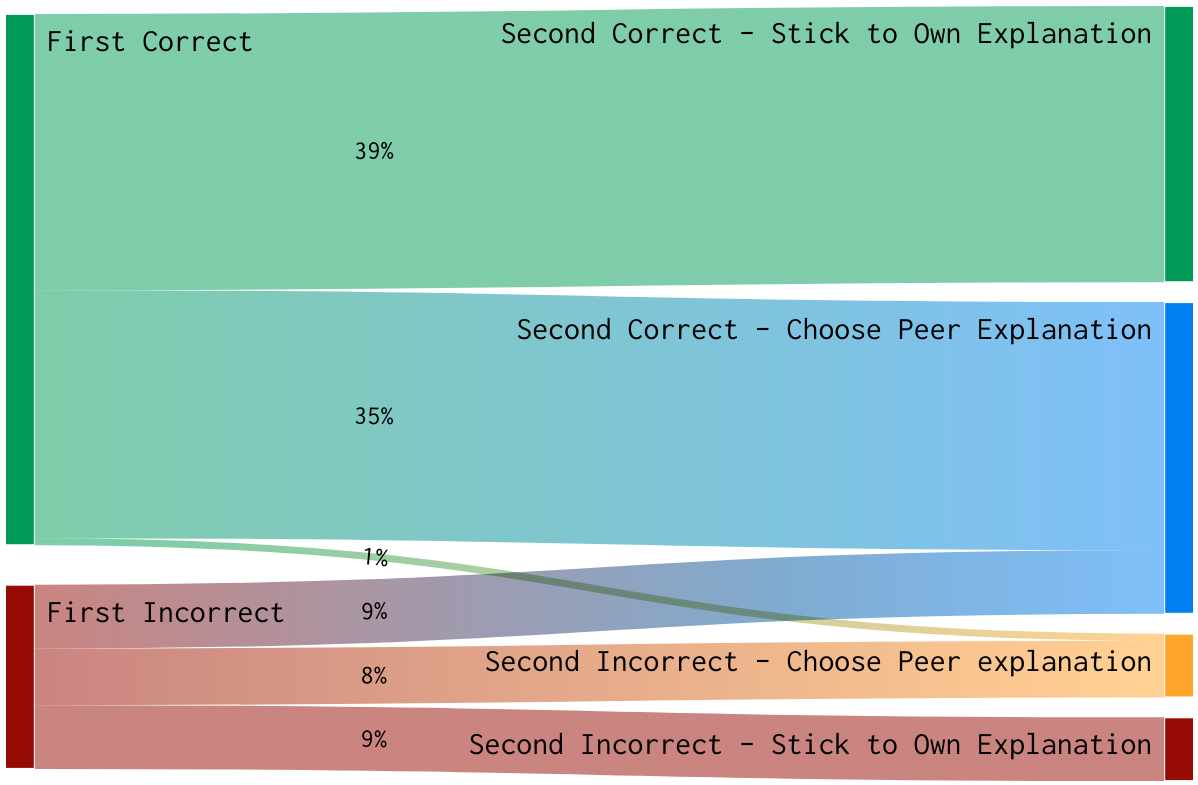
\includegraphics[width=0.7\linewidth]{img/transitions_final.png}
	\caption{The possible transition types that can occur in TMPI for student 
		answers between their first attempt (when they write their own 
		explanation), and the review step (when they are presented with peer 
		explanations). 
		The relative proportion of each transition type is shown in this Sankey 
		diagram for data from myDALITE.org}
	\label{fig:tmpi_sankey}
\end{figure}


The data for this study comes from introductory level university science 
courses (\textbf{Physics} and \textbf{Chemistry}), and generally spans 
different teachers at several colleges and universities in Canada. 
The \textbf{Ethics} dataset comes from the 2013 run of a popular MOOC 
(\textit{Justice}, offered by HarvardX).
The TMPI prompts are slightly different from the \textbf{Physics} and 
\textbf{Chemistry} prompts, in that there is no ``correct'' answer choice, and 
that the goal is to have students choose a side of an argument, and justify 
their choice.
table~\ref{tab:data_summary} gives an overview of the datasets included in this 
study.


\begin{table}
	\caption{
		Summary statistics for reference datasets from argument mining research 
		community and DALITE.
		In the argument reference datasets, \textit{topics} are debate prompts 
		shown to crowdsourcing workers (e.g. \textit{``social media does more 
			good than harm''}), while a \textit{topic} in DALITE is a question 
			item.
		The explanations given by students are analogous to the ``arguments'',  
		which are then assembled into pairs based on what was shown to students.
		\textit{wc} is the average number of tokens in each 
		argument/explanation in each topic.
		Standard deviation of averaged quantities are shown in
		parentheses.
	}
	\label{tab:data_summary}
	\begin{tabular}{llrrrrrrr}
\toprule
       &         &  topics &   args &   pairs & args/topic &  pairs/topic & pairs/arg &       wc \\
source & dataset &         &        &         &            &              &           &          \\
\midrule
Arg Mining & IBM\_ArgQ &      22 &   3474 &    9125 &  158 (144) &    415 (333) &     5 (1) &   24 (1) \\
       & IBM\_Evi &      41 &   1513 &    5274 &    37 (14) &     129 (69) &     7 (3) &   30 (3) \\
       & UKP &      32 &   1052 &   11650 &     33 (3) &     364 (71) &    22 (3) &  49 (14) \\
DALITE & Chemistry &      36 &   4778 &   38742 &   133 (29) &   1076 (313) &     7 (1) &   29 (6) \\
       & Ethics &      28 &  20195 &  159379 &  721 (492) &  5692 (4962) &     7 (1) &   48 (8) \\
       & Physics &      76 &  10840 &   96337 &   143 (42) &   1268 (517) &     7 (2) &   27 (5) \\
\bottomrule
\end{tabular}

\end{table}

To stay consistent with terminology from argument mining research, we 
refer to a question-item as a ``topic''.
The transformation of TMPI student explanations (``args'') into ``pairs'' is 
described in section~\ref{sec:methodology}. 

There are some critical filtering steps taken on raw data before we begin our 
analyses:
\begin{itemize}
	\item Approximately 1 in 10 students decide that they prefer not to have  
	their explanations shared with other students.
	These student answers are removed from the dataset.
	\item We exclude observations where students choose ``\textit{I stick to 
	  my own rationale}''.
	There is a strong bias toward this choice. We consider it may reflect a disengagement and the unwillingness to
        put effort into the task of evaluating all explanations. This filtering reduces our data by approximately 50\%.
	\item Many question items have been completed by several hundreds of 
	students.
	As such, almost half of all student explanations have been shown 
	to another peer; thus we retain only those student answers that were
	presented to at least~5 other students (a threshold we chose based on a 
	qualitative look at the distribution of how often each student explanation 
	has been presented to a peer).
	\item As a platform for formative assessment, not all instructors provide 
	credit for the explanations students write, and there are invariably some 
	students who do not put much effort into writing good explanations.
	We include only those student answers that have at least 10~words.
	\item after the previous two steps, we only include data from those 
	questions that have at least 100 remaining student answers (a threshold 
	chosen based on minimum data required for convergence of BT model in python 
	implementation we use {\href{http://choix.lum.li/en/latest/}{\texttt{choix}}}).
	\item we remove any duplicate pairs before the rank aggregation step that 
	have the same ``winning'' label, as explanations that appear earlier on in 
	the lifetime of a new question are bound to be shown more often to future 
	students.
\end{itemize}


\subsection{Argument Mining Datasets}\label{sec:dataset-AM}
Much of our methodology for the measure for \textit{convincingness} is inspired by work on modelling argument quality, as described in section~\ref{sec:related_work:arg_quality}. 
To contextualize the performance of these methods in our educational 
setting, we apply the same methods to publicly available datasets from the 
AM research community as well and present the results. 
These datasets are described in table~\ref{tab:data_summary}, alongside the 
TMPI data at the heart of our study. 
Each of these datasets was released not just with the labelled argument pairs, 
but holistic rank scores for each argument, which were each derived in different 
ways. 
We will be comparing our proposed measures of \textit{convincingness} to these 
rank scores in section~\ref{sec:methodology_eval}.
\note{commentaire dans PDF du reviewer qui ne nécessite pas de modif?}

The \textbf{UKP} dataset \cite{habernal_which_2016} is one of the first sets of 
labelled argument pairs to be released publicly.
Crowdworkers were presented with pairs of arguments on the same stance of a 
debate prompt, and were asked to choose which was more convincing.
In addition, each argument is assigned a real-valued quality score derived 
from the modified PageRank score described earlier.

The authors of the \textbf{IBM\_ArgQ} dataset \cite{toledo_automatic_2019} 
offer a similarly labelled dataset, but much more tightly curated, with 
strict controls on argument word count and relative length difference in 
each pair.
This curation was partly in response to the observation that, across datasets, crowd 
labels could often be predicted simply by choosing the longer text from the 
pair.
The authors also release in their dataset a real-valued \textit{convincingness} 
score for each argument, which is the average of multiple binary relevance 
judgments provided by Crowdlabellers. 

The labelled argument pairs in the \textbf{IBM\_Evi} dataset 
\cite{gleize_are_2019} are actually generated by scraping Wikipedia, and the 
crowd workers were asked to choose the argument from the pair that provided the 
more compelling evidence in support of the given debate stance.

We see in table~\ref{tab:data_summary} that the different disciplines in our 
TMPI dataset are comparable to the reference AM datasets (just proportionately 
larger).



\section{Proposed methodology to model convincingness}\label{sec:methodology}

We borrow our methodological approach from research in argument mining, 
specifically related to modelling quality along the dimension of 
\textit{convincingness}.
A common approach is to curate pairs of arguments made in defence of the same 
stance on the same topic.
These pairs are then presented to Crowdworkers, whose task is to label  
which of the two is more convincing. 
The pairwise comparisons can then be combined using rank-aggregation methods to produce an overall ordered list of arguments.
We extend this work to the domain of TMPI, and define prediction tasks that not 
only aim to validate this methodology, but help answer our specific research 
questions.\footnote{All code for this project available on 
\href{https://github.com/sameerbhatnagar/convincingness}{Github} (\url{https://github.com/sameerbhatnagar/convincingness}).}

\subsection{Rank Aggregation}\label{sec:rank_agg}
The raw data emerging from a TMPI platform is tabular in the form of 
student-item observations.
We refer to this raw format as \textit{Multiple-choice Explanation} (MCE).
As shown in figure~\ref{fig:make_pairs_a}(a), the data fields in our MCE format 
include: the student's \textit{first} answer choice, their 
accompanying explanation, the peer explanations shown on the review step (as in 
figure~\ref{fig:question_review}), the student's \textit{second} answer choice, 
and finally, the peer explanation they chose as most convincing (\verb|None| if 
they choose to ``stick to their own'').
Timestamps for these events are associated as well.

The process starts by filtering the data in MCE format (described in
section~\ref{sec:dataset_dalite}) to obtain the figure~\ref{fig:tmpi_research}(a) table.
This data is processed into explanation pairs \ref{fig:tmpi_research}(b), which is later
transformed into pointwise convincingness scores \ref{fig:tmpi_research}(c).  When a student
chooses an explanation (other than theirs), pairs are created for all explanations that
were shown as alternatives, including the student's original explanation.  In figure
\ref{fig:tmpi_research}'s example, the choice of e$_{25}$ out of the eight peer explanations
thus results in seven pairs, plus one that includes the student's own.

%    Note that cases of {\em Same answer choice, same explanation} are excluded for the reason that they are unreliable, as suggested by initial experiments where performance is negatively affected.  An hypothesis is that unengaged students have a tendency to not bother making the effort to read and analyze other students' explanations, thereby stiking to their own and adding noise to the data, which in turn degrades performance.

%    Note also that some students may have a tendency to stick with their explanations, while the opposite may also be true.  A student that only chooses their own explanation will end up not contributing any pairs. At the other extreme, a student that never chooses their explanation will penalize these expanations, since a student's own explanation can never be in a winning position in that student's data.

%    Does that tendency result in a bias for the convincingness score?  It could if convincingness correlates with the tendency.  For example, if all strong students stick with their explanation, and all weak students choose a peer's explanation, the weak students' explanations will end up wit with one more loosing pair than the strong students ones'.  This potential bias could be eliminated by excluding all pairs with a student's own explanation, at the expense of reducing the size of the data.  We chose not to, keeping in mind that the potential bias would essentially result in a decrease of performance.

\begin{figure}
	\centering
	\def\svgscale{0.40}
	\input{img/make_pairs_a.pdf_tex}
	\caption{
	Example of student-item observations from a TMPI environment, and the 
	pairwise transformation of data from \textit{Multiple-choice Explanation} 
	format, to \textit{explanation pairs}, to be followed by rank aggregation 
	to produce a sorted list. 
	This figure follows from figure \protect\ref{fig:tmpi}.
	(a) Student~$s_{30}$ chose the correct \textbf{D} as the answer on 
	their first attempt and provided the explanation~$e_{30}$ in the 
	dataset for this question. 
	The student is shown a subset of explanations from previous students for 
	\textbf{D}, as well as for \textbf{A} (the most popular incorrect 
	answer). 
	The student decides to keep the same answer choice \textbf{D}, and 
	indicates that the explanation~$e_{25}$ is the most convincing (\textit{Right}$\rightarrow$\textit{Right} 
	transition).
	(b) This observation is transformed into 8 explanation pairs and indicates
	that~$e_{25}$ is the more convincing of the pair. 
	(c) This pairwise preference data is aggregated into a global, ranked list 
	of student explanations for this question, where each explanation is 
	assigned a real-valued rank score (using the methods described in section 
	\protect\ref{sec:rank_agg}).
}
\label{fig:make_pairs_a}
\end{figure}

We apply the following rank aggregation techniques order to derive a real-valued \textit{convincingness} rank score for each student explanation, as 
depicted in figure~\ref{fig:make_pairs_a}(c).

\begin{enumerate}
	
	\item \textbf{WinRate\_MCE}, defined as the ratio of times an explanation 
	is chosen over the number of times it was shown, calculated from the raw MCE 
	data.
	Since this method is applied before our proposed pairwise transform, it 
	does not take into account \textit{which} peer explanations were shown to 
	each student, neglecting the effect of comparative judgment.
	
	\item \textbf{WinRate}: as described in \citeN{potash_ranking_2019}, this 
	measure of argument quality is defined as the number of times it is chosen 
	as more convincing in a pairwise comparison, normalized for the number of
	pairs in which it appears. 
	In the context of TMPI, when we calculate the \textit{WinRate} of a student 
	explanation after the data transformation depicted in figure 
	\ref{fig:make_pairs_a}a and figure~\ref{fig:make_pairs_a}b, we take a step 
	toward including the effect of comparative judgment, as pairs are 
	specifically constructed for each observation from the explanation that was 
	chosen, and the ones that were shown.
	
	\item \textbf{BT} score, which is the argument ``quality'' parameter 
	estimated for each explanation, according to the \textit{Bradley-Terry} 
	model, where the probability of argument~$a$ being chosen over argument~$b$ 
	is given by:
	
	$$
	P(a>b) = 
	\frac{1}{1+e^{\beta_b-\beta_a}}
	$$
	where~$\beta_i$ is the latent strength parameter of argument~$i$.
	
	We decompose each student-item observation into argument pairs, where the 
	chosen explanation is paired with each of the other shown ones, and the 
	pair is labelled with~$-/+1$, depending on whether the chosen explanation 
	is first/second in the pair.
	Assuming there are~$K$ students, and~$S_k$ pairs labelled by the~$k^{th}$ 
	student, the latent strength parameters are estimated by maximizing 
	the log-likelihood given by:
	$$
	\ell(\boldsymbol{\beta})=\sum_{K}\sum_{(i,j)\epsilon S_k}^{} 
	\log\frac{1}{1+e^{\beta_i - \beta_j}}
	$$
	subject to~$\sum_{i}\beta_i=0$.\footnote{implementation using python 
	library 
	\href{http://choix.lum.li/en/latest/}{\texttt{choix}}}
	
	
	\item The \textbf{Elo} rating system \cite{elo_rating_1978}, which was 
	originally proposed for ranking chess players, has been successfully used 
	in adaptive learning environments (see \citeN{pelanek_applications_2016} 
	for 
	a review). 
	This rating method can be seen as a heuristic re-parametrization of the 
	\textbf{BT} method above, where the probability of argument~$a$ being 
	chosen over argument~$b$ is given by
	$$
	P(a>b) = P_{ab} = \frac{1}{1+10^{(\beta_b-\beta_a)/\delta}}
	$$
	where~$\delta$ is a scaling constant. 
	All arguments are initialized with an initial strength of~$\beta_0$, and 
	the rating of any argument is only updated after it appears in a pairwise 
	comparison with another.
	The rating update rule transfers latent ``strength'' rating points from the 
	loser, to the winner, in proportion to the difference in strength:
	
	$$
	\beta_a':=\beta_a+K(P_{ab} - \beta_a)
	$$
        where $K$ is a factor that can be adjusted to make the score more or less
        sensitive to recent data. It is set to~24 in the current experiments.
	
	While the \textbf{BT} model can be thought of as \textit{consensus} 
	approach (all rank scores are re-calculated after each pair is seen), 
	\textbf{Elo} ratings are dynamic and implicitly give more weight 
	to recent data \cite{aldous_elo_2017}.
	
	\item \textbf{CrowdBT} \cite{chen_pairwise_2013} is an extension of the 
	\textbf{BT} model, tailored to settings where different annotators may have 
	assigned opposite labels to the same pairs and the reliability of each 
	annotator may vary significantly. 
	A reliability parameter~$\eta_k$ is estimated for each student, where the 
	probability that student~$k$ chooses argument~$a$ as more convincing than 
	$b$ is given by 
	
	$$
	\eta_k \equiv P(a >_k b | a >b )
	$$
	
	where~$\eta_k \approx 1$ if the student  $k$ agrees with most other 
	students, and~$\eta_k \approx 0$ if the student is in opposition to their 
	peers.
	This changes the model of argument~$a$ being chosen over~$b$ by student~$k$ 
	to 
	$$
	P(a >_k b) = 
	\eta_k \frac{e^{\beta_a}}{e^{\beta_a}+e^{\beta_b}} + (1-\eta_k) 
	\frac{e^{\beta_b}}{e^{\beta_a}+e^{\beta_b}}
	$$
	and the log-likelihood maximized for estimation to 
	
	$$
	\ell(\boldsymbol{\eta},\boldsymbol{\beta})=\sum_{K}\sum_{(i,j)\epsilon 
		S_K}^{} 
	\log \left[ \eta_k \frac{e^{\beta_a}}{e^{\beta_a}+e^{\beta_b}} + (1-\eta_k) 
	\frac{e^{\beta_b}}{e^{\beta_a}+e^{\beta_b}} \right]
	$$
	
	This method is currently used in the comparative evaluation platform 
	JuxtaPeer \cite{cambre_juxtapeer:_2018}.\footnote{Implementation from 
	\href{https://github.com/anishathalye/gavel/blob/master/gavel/crowd_bt.py}{\texttt{Gavel}}
	 platform.}
	
\end{enumerate}

Section~\ref{sec:methodology_eval} describes how we evaluate the fit of these rank aggregation methods to our data.

\subsection{Linguistic Features}\label{sec:features}
Once the pairwise votes are converted to global ranking scores of convincingness, we next build on these results to predict these 
rankings for each explanation, using different representations of the 
text in those explanations.
We cast \textbf{RQ2}, the goal of identifying the linguistic features behind convincingness, as a regression task, predicting the argument 
\textit{convincingness} scores via a feature-rich document vector.

The list of features included here is derived from related work in argument 
mining \cite{habernal_which_2016,persing_end--end_2016}, on student 
essays and automatic short answer scoring \cite{mohler_text--text_2009}.

\begin{itemize}
	
	\item \textbf{Lexical \& statistical features}: 
	uni-grams, 
	type-token ratio, 
	number of keywords (defined by open-source discipline-specific 
	textbook).
	These features may capture lexical diversity and discipline 
	specific keywords that are predictive of \textit{convincingness}.  Moreover,
	a statistical feature we propose to include is the \textit{number of 
	equations} (captured by a regular expression) used by a student in their 
	explanation, as they appear very often in the TMPI 
	platform data.
	In STEM disciplines, many students choose to reference their knowledge 
	around a body of formulae to justify their reasoning. 
	
	\item \textbf{Syntactic features}: 
	We surmise that such features are question and discipline agnostic and 
	that there are patterns used by students that are simpler to 
	understand for their peers.
	These include part-of-speech (POS) tags (e.g. \textit{noun, preposition, 
	verb, etc.}), and POS bi-grams and tri-grams as well. 
	We replace each word in the student explanation with its universal POS tag
	and derive features from the normalized counts of each of these tags for 
	each student explanation\footnote{POS tagging done using pre-trained models provided with the 
	python package, \href{spacy.io}{\texttt{spacy}}, which uses the tag set defined by 
	the  \href{https://universaldependencies.org/docs/u/pos/}{\textit{Universal 
	Dependencies project}}}.
	We also include counts of certain more detailed 
	Modal verbs (e.g. \textit{must, should, can, might}),
%	contextuality/formality measure \cite{heylighen_variation_2002},
	average height of syntactic parse tree for each sentence.
	
	\item \textbf{Semantic features}: we build from work in automatic short answer 
	grading, which often employs vector space models: student answers are 
	represented as embeddings, and their quality is evaluated based on vector 
	similarity/distance with the embeddings of expert, correct text.
	We make our choice of different embedding spaces based on increasing levels 
	of specificity:  
	\begin{itemize}
		\item Generally available pre-trained GloVe 
		vectors \cite{pennington_glove:_2014} have been used for short-answer 
		grading \cite{magooda_vector_2016,riordan_investigating_2017}. 
		Using the 300-dimensional vectors, we calculate similarity metrics to 
		i) all other explanations (following results from 
		\citeN{gagnon_filtering_2019}), 
		ii) the question item text, and, when available, 
		iii) a teacher provided ``expert'' explanation (feature is \verb|NA| 
		otherwise).
		\item We derive our own discipline-specific embedding vectors, trained 
		on corresponding open-source 
		textbooks\footnote{\href{https://openstax.org}{OpenStax}}. 
		We experiment with a word-based vector space model, Latent Semantic 
		Indexing (\verb|LSI|) \cite{deerwester_indexing_1990}, due to its 
		prevalence in text analytics in educational data mining literature, as 
		well as \verb|Doc2Vec| \cite{le_distributed_2014}, which directly 
		models the compositionality of all the words in a 
		sentence\footnote{model implementations from 
		\href{https://radimrehurek.com/gensim/index.html}{Gensim}}.
		We take the text of the question prompt and, when available, an 
		``expert explanation'' provided by teachers for each question, and 
		determine the 10 most relevant sub-sections of the textbook.
		We then calculate the minimum, maximum, 
		and mean cosine similarity for each student explanation over
                these 10 discipline-specific ``reference texts''.
	\end{itemize}

	These semantic features are meant to leverage the discipline-specific 
	linguistic knowledge contained in reference textbooks.  
		
%	\item Co-reference \cite{persing_end--end_2016}: 
%	fraction of entities from the prompt mentioned in each sentence, 
%	averaged over all sentences (using neural Co-reference resolution)
%	vector cosine similarity between student explanation and prompt, 
%	and answer choices; 
	
	\item \textbf{Readability features} include empirically derived formulas which have 
	been shown to predict how difficult it is to read a text, and which have been 
	used extensively in automatic essay scoring research 
	\cite{graesser_coh-metrix:_2004}.
	The most common indices are the ones we adopt, including  
	Fleish-Kincaid reading ease and grade level,
	Coleman-Liau,
	automated readability index, and 
	a normalized number of spelling errors\footnote{Python package 
	\href{https://pypi.org/project/pyspellchecker/}{PySpellChecker}, 
	which uses Levenshtein distance to determine if any given word is too far 
	from known vocabulary}. 

	
\end{itemize}

Features typical to NLP analyses in the context of writing analytics 
not included here are sentence-to-sentence cohesion, sentiment, and 
psycho-linguistic features, as we deem them not pertinent for shorter responses 
that deal with STEM disciplines.

In our effort to address \textbf{RQ2}, these high dimensional 
feature-rich representations are passed through a uni-variate feature selection 
step, wherein all features are ordered in decreasing order of variance, and the 
top 768 features are retained, to be used as input for the classical regression 
models described earlier.  
We chose this vector representation size to match the size of the contextual 
embeddings in the neural \verb|BERT| models, described in section 
\ref{sec:regress_models}, and compare their performance in a fair manner.
These neural models do not provide the same transparency for interpretation 
upon inspection, but leverage pre-training on massive corpora to bring a broad 
linguistic understanding to our regression task.


\subsection{Regression Models}\label{sec:regress_models}

The machine learning convincingness models we frame as a regression task are
inspired from writing analytics literature, as well as the design objective of 
maximizing interpretability: the ability to inspect models to explain 
predictions of which student answers are most \textit{convincing} is paramount 
in providing pedagogical support to students and teachers.
The models we include in this study are \verb|Linear| regression, 
\verb|Decision Tree| regression, and \verb|Random Forest| regressors.

As demonstrated in related work \cite{habernal_which_2016}, argument 
\verb|Length| is a challenging baseline to beat when modelling 
\textit{convincingness} in pairwise preference data.
While \verb|Length| is not in itself a linguistic nor a
semantic feature, it is likely that
the greater the amount of words, the greater is the opportunity to construct a 
convincing argument. It may also well be a confounding factor that correlates with engagement and, in turn, with convincingness.  Whatever the reason is for its effectiveness, we set explanation \verb|Length| (the number 
of white-space separated tokens) as our regression baseline. 

To provide context with the current state of the art in the prediction of 
argument \textit{convincingness} scores, we also fine-tune a pre-trained 
bi-directional neural transformer model, \verb|BERT|, with argument mining 
reference data sets, as well as the TMPI data from our three disciplines. 
In line with the best-performing model in \citeN{gretz_large-scale_2019}, we go 
beyond this and train a different model where the input is augmented with the 
question prompt. 

The text of the question, along with any text from an accompanying image 
caption, is combined with the student explanation, separated by the 
model-specific \verb|[SEP]| token, and input as a pair of sequences during 
fine-tuning and inference (henceforth be referred to as \verb|BERT_Q)|).

Finally, in the \textbf{Physics} and \textbf{Chemistry} datasets from our TMPI 
platform, many of the questions are accompanied by an \textit{expert} 
explanation, written by the teacher-author of the question (the purpose of 
which is to provide some feedback to the student to read after they have 
submitted their second answer choice in the review step).
We fine-tune a variation of \verb|BERT_Q| and combine \textit{expert}-written 
text, separated by the \verb|SEP| token, with the student explanation, and 
serve as input to the transformer (instead of the topic prompt).
We refer to this approach as \verb|BERT_A|.
The theoretical grounding for the use of these models in the study of 
\textit{convincingness} stems from the different tasks for which the base BERT 
model was originally pre-trained for in \citeN{devlin_bert_2018}.
Firstly, predicting masked words seems to have conferred the BERT 
model with syntactic and semantic knowledge of language.
Second, the next-sentence prediction task seems to be one of the reasons for 
successful transfer learning demonstrated on Glue benchmark tasks, such 
as question-answering and sentence classification. 

In each of \verb|BERT|, \verb|BERT_Q| and \verb|BERT_A|, the contextual 
embedding of the model-specific \verb|[CLS]| token in the last layer of the 
fine-tuned transformer is fed as input into a fully dense regression layer
that outputs a predicted \textit{convincingness} score.

 
\subsection{Evaluation of the proposed methodology}\label{sec:methodology_eval}

In order to address research question \textbf{RQ1} and evaluate the choice of rank
aggregation method, we perform two experiments.  First, we need to
ascertain that we can derive a valid measure of convincingness given a set of pairwise
comparisons of explanations.  This is accomplished by comparing the calculated score with an
independent external score obtained from human judgements (external validity experiment),
and by measuring how the calculated score can reliably predict back the pairwise order
in a cross-validation scheme (internal validity experiment).

Finally, we address \textbf{RQ2} by comparing a range of models that use the
convincingness score as the ground truth for training.  Each model varies in how it uses
linguistic features to predict convincingness.  
generalization

\subsubsection{External validity of the convincingness score}
We begin by measuring the correlation between the scores output from the rank 
aggregation methods described in section~\ref{sec:rank_agg}, and the 
``reference'' scores provided with the AM datasets obtained from Crowdlabellers (outlined in section \ref{sec:dataset-AM}).
For each topic in the different AM datasets, we calculate the Pearson 
correlation between the ``reference'' scores of each argument, and 
\textit{WinRate}, \textit{BT}, \textit{Elo} scores aggregated from the pairwise 
preference data. (We cannot include \textit{CrowdBT} here, as the AM datasets 
do not include information on which crowd workers labelled which argument 
pairs, which is a requirement for estimating the annotator-specific~$\eta_k$).
The distribution of Pearson correlation coefficients across the different 
topics for each dataset is shown in the box plots in figure 
\ref{fig:corr_to_reference_score}.

\begin{figure}[H]
	\centering
	\scalebox{0.5}{%% Creator: Matplotlib, PGF backend
%%
%% To include the figure in your LaTeX document, write
%%   \input{<filename>.pgf}
%%
%% Make sure the required packages are loaded in your preamble
%%   \usepackage{pgf}
%%
%% and, on pdftex
%%   \usepackage[utf8]{inputenc}\DeclareUnicodeCharacter{2212}{-}
%%
%% or, on luatex and xetex
%%   \usepackage{unicode-math}
%%
%% Figures using additional raster images can only be included by \input if
%% they are in the same directory as the main LaTeX file. For loading figures
%% from other directories you can use the `import` package
%%   \usepackage{import}
%%
%% and then include the figures with
%%   \import{<path to file>}{<filename>.pgf}
%%
%% Matplotlib used the following preamble
%%
\begingroup%
\makeatletter%
\begin{pgfpicture}%
\pgfpathrectangle{\pgfpointorigin}{\pgfqpoint{9.000000in}{6.000000in}}%
\pgfusepath{use as bounding box, clip}%
\begin{pgfscope}%
\pgfsetbuttcap%
\pgfsetmiterjoin%
\definecolor{currentfill}{rgb}{1.000000,1.000000,1.000000}%
\pgfsetfillcolor{currentfill}%
\pgfsetlinewidth{0.000000pt}%
\definecolor{currentstroke}{rgb}{1.000000,1.000000,1.000000}%
\pgfsetstrokecolor{currentstroke}%
\pgfsetdash{}{0pt}%
\pgfpathmoveto{\pgfqpoint{0.000000in}{0.000000in}}%
\pgfpathlineto{\pgfqpoint{9.000000in}{0.000000in}}%
\pgfpathlineto{\pgfqpoint{9.000000in}{6.000000in}}%
\pgfpathlineto{\pgfqpoint{0.000000in}{6.000000in}}%
\pgfpathclose%
\pgfusepath{fill}%
\end{pgfscope}%
\begin{pgfscope}%
\pgfsetbuttcap%
\pgfsetmiterjoin%
\definecolor{currentfill}{rgb}{0.898039,0.898039,0.898039}%
\pgfsetfillcolor{currentfill}%
\pgfsetlinewidth{0.000000pt}%
\definecolor{currentstroke}{rgb}{0.000000,0.000000,0.000000}%
\pgfsetstrokecolor{currentstroke}%
\pgfsetstrokeopacity{0.000000}%
\pgfsetdash{}{0pt}%
\pgfpathmoveto{\pgfqpoint{1.125000in}{0.660000in}}%
\pgfpathlineto{\pgfqpoint{8.100000in}{0.660000in}}%
\pgfpathlineto{\pgfqpoint{8.100000in}{5.280000in}}%
\pgfpathlineto{\pgfqpoint{1.125000in}{5.280000in}}%
\pgfpathclose%
\pgfusepath{fill}%
\end{pgfscope}%
\begin{pgfscope}%
\pgfsetbuttcap%
\pgfsetroundjoin%
\definecolor{currentfill}{rgb}{0.333333,0.333333,0.333333}%
\pgfsetfillcolor{currentfill}%
\pgfsetlinewidth{0.803000pt}%
\definecolor{currentstroke}{rgb}{0.333333,0.333333,0.333333}%
\pgfsetstrokecolor{currentstroke}%
\pgfsetdash{}{0pt}%
\pgfsys@defobject{currentmarker}{\pgfqpoint{0.000000in}{-0.048611in}}{\pgfqpoint{0.000000in}{0.000000in}}{%
\pgfpathmoveto{\pgfqpoint{0.000000in}{0.000000in}}%
\pgfpathlineto{\pgfqpoint{0.000000in}{-0.048611in}}%
\pgfusepath{stroke,fill}%
}%
\begin{pgfscope}%
\pgfsys@transformshift{2.287500in}{0.660000in}%
\pgfsys@useobject{currentmarker}{}%
\end{pgfscope}%
\end{pgfscope}%
\begin{pgfscope}%
\definecolor{textcolor}{rgb}{0.333333,0.333333,0.333333}%
\pgfsetstrokecolor{textcolor}%
\pgfsetfillcolor{textcolor}%
\pgftext[x=2.287500in,y=0.562778in,,top]{\color{textcolor}\rmfamily\fontsize{10.000000}{12.000000}\selectfont IBM\_ArgQ}%
\end{pgfscope}%
\begin{pgfscope}%
\pgfsetbuttcap%
\pgfsetroundjoin%
\definecolor{currentfill}{rgb}{0.333333,0.333333,0.333333}%
\pgfsetfillcolor{currentfill}%
\pgfsetlinewidth{0.803000pt}%
\definecolor{currentstroke}{rgb}{0.333333,0.333333,0.333333}%
\pgfsetstrokecolor{currentstroke}%
\pgfsetdash{}{0pt}%
\pgfsys@defobject{currentmarker}{\pgfqpoint{0.000000in}{-0.048611in}}{\pgfqpoint{0.000000in}{0.000000in}}{%
\pgfpathmoveto{\pgfqpoint{0.000000in}{0.000000in}}%
\pgfpathlineto{\pgfqpoint{0.000000in}{-0.048611in}}%
\pgfusepath{stroke,fill}%
}%
\begin{pgfscope}%
\pgfsys@transformshift{4.612500in}{0.660000in}%
\pgfsys@useobject{currentmarker}{}%
\end{pgfscope}%
\end{pgfscope}%
\begin{pgfscope}%
\definecolor{textcolor}{rgb}{0.333333,0.333333,0.333333}%
\pgfsetstrokecolor{textcolor}%
\pgfsetfillcolor{textcolor}%
\pgftext[x=4.612500in,y=0.562778in,,top]{\color{textcolor}\rmfamily\fontsize{10.000000}{12.000000}\selectfont IBM\_Evi}%
\end{pgfscope}%
\begin{pgfscope}%
\pgfsetbuttcap%
\pgfsetroundjoin%
\definecolor{currentfill}{rgb}{0.333333,0.333333,0.333333}%
\pgfsetfillcolor{currentfill}%
\pgfsetlinewidth{0.803000pt}%
\definecolor{currentstroke}{rgb}{0.333333,0.333333,0.333333}%
\pgfsetstrokecolor{currentstroke}%
\pgfsetdash{}{0pt}%
\pgfsys@defobject{currentmarker}{\pgfqpoint{0.000000in}{-0.048611in}}{\pgfqpoint{0.000000in}{0.000000in}}{%
\pgfpathmoveto{\pgfqpoint{0.000000in}{0.000000in}}%
\pgfpathlineto{\pgfqpoint{0.000000in}{-0.048611in}}%
\pgfusepath{stroke,fill}%
}%
\begin{pgfscope}%
\pgfsys@transformshift{6.937500in}{0.660000in}%
\pgfsys@useobject{currentmarker}{}%
\end{pgfscope}%
\end{pgfscope}%
\begin{pgfscope}%
\definecolor{textcolor}{rgb}{0.333333,0.333333,0.333333}%
\pgfsetstrokecolor{textcolor}%
\pgfsetfillcolor{textcolor}%
\pgftext[x=6.937500in,y=0.562778in,,top]{\color{textcolor}\rmfamily\fontsize{10.000000}{12.000000}\selectfont UKP}%
\end{pgfscope}%
\begin{pgfscope}%
\definecolor{textcolor}{rgb}{0.333333,0.333333,0.333333}%
\pgfsetstrokecolor{textcolor}%
\pgfsetfillcolor{textcolor}%
\pgftext[x=4.612500in,y=0.383766in,,top]{\color{textcolor}\rmfamily\fontsize{12.000000}{14.400000}\selectfont Dataset}%
\end{pgfscope}%
\begin{pgfscope}%
\pgfpathrectangle{\pgfqpoint{1.125000in}{0.660000in}}{\pgfqpoint{6.975000in}{4.620000in}}%
\pgfusepath{clip}%
\pgfsetrectcap%
\pgfsetroundjoin%
\pgfsetlinewidth{0.803000pt}%
\definecolor{currentstroke}{rgb}{1.000000,1.000000,1.000000}%
\pgfsetstrokecolor{currentstroke}%
\pgfsetdash{}{0pt}%
\pgfpathmoveto{\pgfqpoint{1.125000in}{0.820588in}}%
\pgfpathlineto{\pgfqpoint{8.100000in}{0.820588in}}%
\pgfusepath{stroke}%
\end{pgfscope}%
\begin{pgfscope}%
\pgfsetbuttcap%
\pgfsetroundjoin%
\definecolor{currentfill}{rgb}{0.333333,0.333333,0.333333}%
\pgfsetfillcolor{currentfill}%
\pgfsetlinewidth{0.803000pt}%
\definecolor{currentstroke}{rgb}{0.333333,0.333333,0.333333}%
\pgfsetstrokecolor{currentstroke}%
\pgfsetdash{}{0pt}%
\pgfsys@defobject{currentmarker}{\pgfqpoint{-0.048611in}{0.000000in}}{\pgfqpoint{0.000000in}{0.000000in}}{%
\pgfpathmoveto{\pgfqpoint{0.000000in}{0.000000in}}%
\pgfpathlineto{\pgfqpoint{-0.048611in}{0.000000in}}%
\pgfusepath{stroke,fill}%
}%
\begin{pgfscope}%
\pgfsys@transformshift{1.125000in}{0.820588in}%
\pgfsys@useobject{currentmarker}{}%
\end{pgfscope}%
\end{pgfscope}%
\begin{pgfscope}%
\definecolor{textcolor}{rgb}{0.333333,0.333333,0.333333}%
\pgfsetstrokecolor{textcolor}%
\pgfsetfillcolor{textcolor}%
\pgftext[x=0.850308in, y=0.772363in, left, base]{\color{textcolor}\rmfamily\fontsize{10.000000}{12.000000}\selectfont \(\displaystyle 0.0\)}%
\end{pgfscope}%
\begin{pgfscope}%
\pgfpathrectangle{\pgfqpoint{1.125000in}{0.660000in}}{\pgfqpoint{6.975000in}{4.620000in}}%
\pgfusepath{clip}%
\pgfsetrectcap%
\pgfsetroundjoin%
\pgfsetlinewidth{0.803000pt}%
\definecolor{currentstroke}{rgb}{1.000000,1.000000,1.000000}%
\pgfsetstrokecolor{currentstroke}%
\pgfsetdash{}{0pt}%
\pgfpathmoveto{\pgfqpoint{1.125000in}{1.808824in}}%
\pgfpathlineto{\pgfqpoint{8.100000in}{1.808824in}}%
\pgfusepath{stroke}%
\end{pgfscope}%
\begin{pgfscope}%
\pgfsetbuttcap%
\pgfsetroundjoin%
\definecolor{currentfill}{rgb}{0.333333,0.333333,0.333333}%
\pgfsetfillcolor{currentfill}%
\pgfsetlinewidth{0.803000pt}%
\definecolor{currentstroke}{rgb}{0.333333,0.333333,0.333333}%
\pgfsetstrokecolor{currentstroke}%
\pgfsetdash{}{0pt}%
\pgfsys@defobject{currentmarker}{\pgfqpoint{-0.048611in}{0.000000in}}{\pgfqpoint{0.000000in}{0.000000in}}{%
\pgfpathmoveto{\pgfqpoint{0.000000in}{0.000000in}}%
\pgfpathlineto{\pgfqpoint{-0.048611in}{0.000000in}}%
\pgfusepath{stroke,fill}%
}%
\begin{pgfscope}%
\pgfsys@transformshift{1.125000in}{1.808824in}%
\pgfsys@useobject{currentmarker}{}%
\end{pgfscope}%
\end{pgfscope}%
\begin{pgfscope}%
\definecolor{textcolor}{rgb}{0.333333,0.333333,0.333333}%
\pgfsetstrokecolor{textcolor}%
\pgfsetfillcolor{textcolor}%
\pgftext[x=0.850308in, y=1.760598in, left, base]{\color{textcolor}\rmfamily\fontsize{10.000000}{12.000000}\selectfont \(\displaystyle 0.2\)}%
\end{pgfscope}%
\begin{pgfscope}%
\pgfpathrectangle{\pgfqpoint{1.125000in}{0.660000in}}{\pgfqpoint{6.975000in}{4.620000in}}%
\pgfusepath{clip}%
\pgfsetrectcap%
\pgfsetroundjoin%
\pgfsetlinewidth{0.803000pt}%
\definecolor{currentstroke}{rgb}{1.000000,1.000000,1.000000}%
\pgfsetstrokecolor{currentstroke}%
\pgfsetdash{}{0pt}%
\pgfpathmoveto{\pgfqpoint{1.125000in}{2.797059in}}%
\pgfpathlineto{\pgfqpoint{8.100000in}{2.797059in}}%
\pgfusepath{stroke}%
\end{pgfscope}%
\begin{pgfscope}%
\pgfsetbuttcap%
\pgfsetroundjoin%
\definecolor{currentfill}{rgb}{0.333333,0.333333,0.333333}%
\pgfsetfillcolor{currentfill}%
\pgfsetlinewidth{0.803000pt}%
\definecolor{currentstroke}{rgb}{0.333333,0.333333,0.333333}%
\pgfsetstrokecolor{currentstroke}%
\pgfsetdash{}{0pt}%
\pgfsys@defobject{currentmarker}{\pgfqpoint{-0.048611in}{0.000000in}}{\pgfqpoint{0.000000in}{0.000000in}}{%
\pgfpathmoveto{\pgfqpoint{0.000000in}{0.000000in}}%
\pgfpathlineto{\pgfqpoint{-0.048611in}{0.000000in}}%
\pgfusepath{stroke,fill}%
}%
\begin{pgfscope}%
\pgfsys@transformshift{1.125000in}{2.797059in}%
\pgfsys@useobject{currentmarker}{}%
\end{pgfscope}%
\end{pgfscope}%
\begin{pgfscope}%
\definecolor{textcolor}{rgb}{0.333333,0.333333,0.333333}%
\pgfsetstrokecolor{textcolor}%
\pgfsetfillcolor{textcolor}%
\pgftext[x=0.850308in, y=2.748834in, left, base]{\color{textcolor}\rmfamily\fontsize{10.000000}{12.000000}\selectfont \(\displaystyle 0.4\)}%
\end{pgfscope}%
\begin{pgfscope}%
\pgfpathrectangle{\pgfqpoint{1.125000in}{0.660000in}}{\pgfqpoint{6.975000in}{4.620000in}}%
\pgfusepath{clip}%
\pgfsetrectcap%
\pgfsetroundjoin%
\pgfsetlinewidth{0.803000pt}%
\definecolor{currentstroke}{rgb}{1.000000,1.000000,1.000000}%
\pgfsetstrokecolor{currentstroke}%
\pgfsetdash{}{0pt}%
\pgfpathmoveto{\pgfqpoint{1.125000in}{3.785294in}}%
\pgfpathlineto{\pgfqpoint{8.100000in}{3.785294in}}%
\pgfusepath{stroke}%
\end{pgfscope}%
\begin{pgfscope}%
\pgfsetbuttcap%
\pgfsetroundjoin%
\definecolor{currentfill}{rgb}{0.333333,0.333333,0.333333}%
\pgfsetfillcolor{currentfill}%
\pgfsetlinewidth{0.803000pt}%
\definecolor{currentstroke}{rgb}{0.333333,0.333333,0.333333}%
\pgfsetstrokecolor{currentstroke}%
\pgfsetdash{}{0pt}%
\pgfsys@defobject{currentmarker}{\pgfqpoint{-0.048611in}{0.000000in}}{\pgfqpoint{0.000000in}{0.000000in}}{%
\pgfpathmoveto{\pgfqpoint{0.000000in}{0.000000in}}%
\pgfpathlineto{\pgfqpoint{-0.048611in}{0.000000in}}%
\pgfusepath{stroke,fill}%
}%
\begin{pgfscope}%
\pgfsys@transformshift{1.125000in}{3.785294in}%
\pgfsys@useobject{currentmarker}{}%
\end{pgfscope}%
\end{pgfscope}%
\begin{pgfscope}%
\definecolor{textcolor}{rgb}{0.333333,0.333333,0.333333}%
\pgfsetstrokecolor{textcolor}%
\pgfsetfillcolor{textcolor}%
\pgftext[x=0.850308in, y=3.737069in, left, base]{\color{textcolor}\rmfamily\fontsize{10.000000}{12.000000}\selectfont \(\displaystyle 0.6\)}%
\end{pgfscope}%
\begin{pgfscope}%
\pgfpathrectangle{\pgfqpoint{1.125000in}{0.660000in}}{\pgfqpoint{6.975000in}{4.620000in}}%
\pgfusepath{clip}%
\pgfsetrectcap%
\pgfsetroundjoin%
\pgfsetlinewidth{0.803000pt}%
\definecolor{currentstroke}{rgb}{1.000000,1.000000,1.000000}%
\pgfsetstrokecolor{currentstroke}%
\pgfsetdash{}{0pt}%
\pgfpathmoveto{\pgfqpoint{1.125000in}{4.773529in}}%
\pgfpathlineto{\pgfqpoint{8.100000in}{4.773529in}}%
\pgfusepath{stroke}%
\end{pgfscope}%
\begin{pgfscope}%
\pgfsetbuttcap%
\pgfsetroundjoin%
\definecolor{currentfill}{rgb}{0.333333,0.333333,0.333333}%
\pgfsetfillcolor{currentfill}%
\pgfsetlinewidth{0.803000pt}%
\definecolor{currentstroke}{rgb}{0.333333,0.333333,0.333333}%
\pgfsetstrokecolor{currentstroke}%
\pgfsetdash{}{0pt}%
\pgfsys@defobject{currentmarker}{\pgfqpoint{-0.048611in}{0.000000in}}{\pgfqpoint{0.000000in}{0.000000in}}{%
\pgfpathmoveto{\pgfqpoint{0.000000in}{0.000000in}}%
\pgfpathlineto{\pgfqpoint{-0.048611in}{0.000000in}}%
\pgfusepath{stroke,fill}%
}%
\begin{pgfscope}%
\pgfsys@transformshift{1.125000in}{4.773529in}%
\pgfsys@useobject{currentmarker}{}%
\end{pgfscope}%
\end{pgfscope}%
\begin{pgfscope}%
\definecolor{textcolor}{rgb}{0.333333,0.333333,0.333333}%
\pgfsetstrokecolor{textcolor}%
\pgfsetfillcolor{textcolor}%
\pgftext[x=0.850308in, y=4.725304in, left, base]{\color{textcolor}\rmfamily\fontsize{10.000000}{12.000000}\selectfont \(\displaystyle 0.8\)}%
\end{pgfscope}%
\begin{pgfscope}%
\definecolor{textcolor}{rgb}{0.333333,0.333333,0.333333}%
\pgfsetstrokecolor{textcolor}%
\pgfsetfillcolor{textcolor}%
\pgftext[x=0.794752in,y=2.970000in,,bottom,rotate=90.000000]{\color{textcolor}\rmfamily\fontsize{12.000000}{14.400000}\selectfont Correlation to Reference Score}%
\end{pgfscope}%
\begin{pgfscope}%
\pgfpathrectangle{\pgfqpoint{1.125000in}{0.660000in}}{\pgfqpoint{6.975000in}{4.620000in}}%
\pgfusepath{clip}%
\pgfsetbuttcap%
\pgfsetmiterjoin%
\definecolor{currentfill}{rgb}{0.800490,0.353431,0.285784}%
\pgfsetfillcolor{currentfill}%
\pgfsetlinewidth{1.505625pt}%
\definecolor{currentstroke}{rgb}{0.282353,0.282353,0.282353}%
\pgfsetstrokecolor{currentstroke}%
\pgfsetdash{}{0pt}%
\pgfpathmoveto{\pgfqpoint{1.363700in}{3.118235in}}%
\pgfpathlineto{\pgfqpoint{1.971300in}{3.118235in}}%
\pgfpathlineto{\pgfqpoint{1.971300in}{3.921176in}}%
\pgfpathlineto{\pgfqpoint{1.363700in}{3.921176in}}%
\pgfpathlineto{\pgfqpoint{1.363700in}{3.118235in}}%
\pgfpathclose%
\pgfusepath{stroke,fill}%
\end{pgfscope}%
\begin{pgfscope}%
\pgfpathrectangle{\pgfqpoint{1.125000in}{0.660000in}}{\pgfqpoint{6.975000in}{4.620000in}}%
\pgfusepath{clip}%
\pgfsetbuttcap%
\pgfsetmiterjoin%
\definecolor{currentfill}{rgb}{0.271078,0.524020,0.674020}%
\pgfsetfillcolor{currentfill}%
\pgfsetlinewidth{1.505625pt}%
\definecolor{currentstroke}{rgb}{0.282353,0.282353,0.282353}%
\pgfsetstrokecolor{currentstroke}%
\pgfsetdash{}{0pt}%
\pgfpathmoveto{\pgfqpoint{1.983700in}{3.204706in}}%
\pgfpathlineto{\pgfqpoint{2.591300in}{3.204706in}}%
\pgfpathlineto{\pgfqpoint{2.591300in}{4.118824in}}%
\pgfpathlineto{\pgfqpoint{1.983700in}{4.118824in}}%
\pgfpathlineto{\pgfqpoint{1.983700in}{3.204706in}}%
\pgfpathclose%
\pgfusepath{stroke,fill}%
\end{pgfscope}%
\begin{pgfscope}%
\pgfpathrectangle{\pgfqpoint{1.125000in}{0.660000in}}{\pgfqpoint{6.975000in}{4.620000in}}%
\pgfusepath{clip}%
\pgfsetbuttcap%
\pgfsetmiterjoin%
\definecolor{currentfill}{rgb}{0.621078,0.591667,0.800490}%
\pgfsetfillcolor{currentfill}%
\pgfsetlinewidth{1.505625pt}%
\definecolor{currentstroke}{rgb}{0.282353,0.282353,0.282353}%
\pgfsetstrokecolor{currentstroke}%
\pgfsetdash{}{0pt}%
\pgfpathmoveto{\pgfqpoint{2.603700in}{3.550588in}}%
\pgfpathlineto{\pgfqpoint{3.211300in}{3.550588in}}%
\pgfpathlineto{\pgfqpoint{3.211300in}{4.254706in}}%
\pgfpathlineto{\pgfqpoint{2.603700in}{4.254706in}}%
\pgfpathlineto{\pgfqpoint{2.603700in}{3.550588in}}%
\pgfpathclose%
\pgfusepath{stroke,fill}%
\end{pgfscope}%
\begin{pgfscope}%
\pgfpathrectangle{\pgfqpoint{1.125000in}{0.660000in}}{\pgfqpoint{6.975000in}{4.620000in}}%
\pgfusepath{clip}%
\pgfsetbuttcap%
\pgfsetmiterjoin%
\definecolor{currentfill}{rgb}{0.800490,0.353431,0.285784}%
\pgfsetfillcolor{currentfill}%
\pgfsetlinewidth{1.505625pt}%
\definecolor{currentstroke}{rgb}{0.282353,0.282353,0.282353}%
\pgfsetstrokecolor{currentstroke}%
\pgfsetdash{}{0pt}%
\pgfpathmoveto{\pgfqpoint{3.688700in}{1.660588in}}%
\pgfpathlineto{\pgfqpoint{4.296300in}{1.660588in}}%
\pgfpathlineto{\pgfqpoint{4.296300in}{2.747647in}}%
\pgfpathlineto{\pgfqpoint{3.688700in}{2.747647in}}%
\pgfpathlineto{\pgfqpoint{3.688700in}{1.660588in}}%
\pgfpathclose%
\pgfusepath{stroke,fill}%
\end{pgfscope}%
\begin{pgfscope}%
\pgfpathrectangle{\pgfqpoint{1.125000in}{0.660000in}}{\pgfqpoint{6.975000in}{4.620000in}}%
\pgfusepath{clip}%
\pgfsetbuttcap%
\pgfsetmiterjoin%
\definecolor{currentfill}{rgb}{0.271078,0.524020,0.674020}%
\pgfsetfillcolor{currentfill}%
\pgfsetlinewidth{1.505625pt}%
\definecolor{currentstroke}{rgb}{0.282353,0.282353,0.282353}%
\pgfsetstrokecolor{currentstroke}%
\pgfsetdash{}{0pt}%
\pgfpathmoveto{\pgfqpoint{4.308700in}{1.462941in}}%
\pgfpathlineto{\pgfqpoint{4.916300in}{1.462941in}}%
\pgfpathlineto{\pgfqpoint{4.916300in}{2.994706in}}%
\pgfpathlineto{\pgfqpoint{4.308700in}{2.994706in}}%
\pgfpathlineto{\pgfqpoint{4.308700in}{1.462941in}}%
\pgfpathclose%
\pgfusepath{stroke,fill}%
\end{pgfscope}%
\begin{pgfscope}%
\pgfpathrectangle{\pgfqpoint{1.125000in}{0.660000in}}{\pgfqpoint{6.975000in}{4.620000in}}%
\pgfusepath{clip}%
\pgfsetbuttcap%
\pgfsetmiterjoin%
\definecolor{currentfill}{rgb}{0.621078,0.591667,0.800490}%
\pgfsetfillcolor{currentfill}%
\pgfsetlinewidth{1.505625pt}%
\definecolor{currentstroke}{rgb}{0.282353,0.282353,0.282353}%
\pgfsetstrokecolor{currentstroke}%
\pgfsetdash{}{0pt}%
\pgfpathmoveto{\pgfqpoint{4.928700in}{1.710000in}}%
\pgfpathlineto{\pgfqpoint{5.536300in}{1.710000in}}%
\pgfpathlineto{\pgfqpoint{5.536300in}{2.846471in}}%
\pgfpathlineto{\pgfqpoint{4.928700in}{2.846471in}}%
\pgfpathlineto{\pgfqpoint{4.928700in}{1.710000in}}%
\pgfpathclose%
\pgfusepath{stroke,fill}%
\end{pgfscope}%
\begin{pgfscope}%
\pgfpathrectangle{\pgfqpoint{1.125000in}{0.660000in}}{\pgfqpoint{6.975000in}{4.620000in}}%
\pgfusepath{clip}%
\pgfsetbuttcap%
\pgfsetmiterjoin%
\definecolor{currentfill}{rgb}{0.800490,0.353431,0.285784}%
\pgfsetfillcolor{currentfill}%
\pgfsetlinewidth{1.505625pt}%
\definecolor{currentstroke}{rgb}{0.282353,0.282353,0.282353}%
\pgfsetstrokecolor{currentstroke}%
\pgfsetdash{}{0pt}%
\pgfpathmoveto{\pgfqpoint{6.013700in}{3.377647in}}%
\pgfpathlineto{\pgfqpoint{6.621300in}{3.377647in}}%
\pgfpathlineto{\pgfqpoint{6.621300in}{4.069412in}}%
\pgfpathlineto{\pgfqpoint{6.013700in}{4.069412in}}%
\pgfpathlineto{\pgfqpoint{6.013700in}{3.377647in}}%
\pgfpathclose%
\pgfusepath{stroke,fill}%
\end{pgfscope}%
\begin{pgfscope}%
\pgfpathrectangle{\pgfqpoint{1.125000in}{0.660000in}}{\pgfqpoint{6.975000in}{4.620000in}}%
\pgfusepath{clip}%
\pgfsetbuttcap%
\pgfsetmiterjoin%
\definecolor{currentfill}{rgb}{0.271078,0.524020,0.674020}%
\pgfsetfillcolor{currentfill}%
\pgfsetlinewidth{1.505625pt}%
\definecolor{currentstroke}{rgb}{0.282353,0.282353,0.282353}%
\pgfsetstrokecolor{currentstroke}%
\pgfsetdash{}{0pt}%
\pgfpathmoveto{\pgfqpoint{6.633700in}{4.118824in}}%
\pgfpathlineto{\pgfqpoint{7.241300in}{4.118824in}}%
\pgfpathlineto{\pgfqpoint{7.241300in}{4.538824in}}%
\pgfpathlineto{\pgfqpoint{6.633700in}{4.538824in}}%
\pgfpathlineto{\pgfqpoint{6.633700in}{4.118824in}}%
\pgfpathclose%
\pgfusepath{stroke,fill}%
\end{pgfscope}%
\begin{pgfscope}%
\pgfpathrectangle{\pgfqpoint{1.125000in}{0.660000in}}{\pgfqpoint{6.975000in}{4.620000in}}%
\pgfusepath{clip}%
\pgfsetbuttcap%
\pgfsetmiterjoin%
\definecolor{currentfill}{rgb}{0.621078,0.591667,0.800490}%
\pgfsetfillcolor{currentfill}%
\pgfsetlinewidth{1.505625pt}%
\definecolor{currentstroke}{rgb}{0.282353,0.282353,0.282353}%
\pgfsetstrokecolor{currentstroke}%
\pgfsetdash{}{0pt}%
\pgfpathmoveto{\pgfqpoint{7.253700in}{3.760588in}}%
\pgfpathlineto{\pgfqpoint{7.861300in}{3.760588in}}%
\pgfpathlineto{\pgfqpoint{7.861300in}{4.291765in}}%
\pgfpathlineto{\pgfqpoint{7.253700in}{4.291765in}}%
\pgfpathlineto{\pgfqpoint{7.253700in}{3.760588in}}%
\pgfpathclose%
\pgfusepath{stroke,fill}%
\end{pgfscope}%
\begin{pgfscope}%
\pgfpathrectangle{\pgfqpoint{1.125000in}{0.660000in}}{\pgfqpoint{6.975000in}{4.620000in}}%
\pgfusepath{clip}%
\pgfsetbuttcap%
\pgfsetmiterjoin%
\definecolor{currentfill}{rgb}{0.800490,0.353431,0.285784}%
\pgfsetfillcolor{currentfill}%
\pgfsetlinewidth{0.752812pt}%
\definecolor{currentstroke}{rgb}{0.282353,0.282353,0.282353}%
\pgfsetstrokecolor{currentstroke}%
\pgfsetdash{}{0pt}%
\pgfpathmoveto{\pgfqpoint{2.287500in}{0.820588in}}%
\pgfpathlineto{\pgfqpoint{2.287500in}{0.820588in}}%
\pgfpathlineto{\pgfqpoint{2.287500in}{0.820588in}}%
\pgfpathlineto{\pgfqpoint{2.287500in}{0.820588in}}%
\pgfpathclose%
\pgfusepath{stroke,fill}%
\end{pgfscope}%
\begin{pgfscope}%
\pgfpathrectangle{\pgfqpoint{1.125000in}{0.660000in}}{\pgfqpoint{6.975000in}{4.620000in}}%
\pgfusepath{clip}%
\pgfsetbuttcap%
\pgfsetmiterjoin%
\definecolor{currentfill}{rgb}{0.271078,0.524020,0.674020}%
\pgfsetfillcolor{currentfill}%
\pgfsetlinewidth{0.752812pt}%
\definecolor{currentstroke}{rgb}{0.282353,0.282353,0.282353}%
\pgfsetstrokecolor{currentstroke}%
\pgfsetdash{}{0pt}%
\pgfpathmoveto{\pgfqpoint{2.287500in}{0.820588in}}%
\pgfpathlineto{\pgfqpoint{2.287500in}{0.820588in}}%
\pgfpathlineto{\pgfqpoint{2.287500in}{0.820588in}}%
\pgfpathlineto{\pgfqpoint{2.287500in}{0.820588in}}%
\pgfpathclose%
\pgfusepath{stroke,fill}%
\end{pgfscope}%
\begin{pgfscope}%
\pgfpathrectangle{\pgfqpoint{1.125000in}{0.660000in}}{\pgfqpoint{6.975000in}{4.620000in}}%
\pgfusepath{clip}%
\pgfsetbuttcap%
\pgfsetmiterjoin%
\definecolor{currentfill}{rgb}{0.621078,0.591667,0.800490}%
\pgfsetfillcolor{currentfill}%
\pgfsetlinewidth{0.752812pt}%
\definecolor{currentstroke}{rgb}{0.282353,0.282353,0.282353}%
\pgfsetstrokecolor{currentstroke}%
\pgfsetdash{}{0pt}%
\pgfpathmoveto{\pgfqpoint{2.287500in}{0.820588in}}%
\pgfpathlineto{\pgfqpoint{2.287500in}{0.820588in}}%
\pgfpathlineto{\pgfqpoint{2.287500in}{0.820588in}}%
\pgfpathlineto{\pgfqpoint{2.287500in}{0.820588in}}%
\pgfpathclose%
\pgfusepath{stroke,fill}%
\end{pgfscope}%
\begin{pgfscope}%
\pgfpathrectangle{\pgfqpoint{1.125000in}{0.660000in}}{\pgfqpoint{6.975000in}{4.620000in}}%
\pgfusepath{clip}%
\pgfsetrectcap%
\pgfsetroundjoin%
\pgfsetlinewidth{1.505625pt}%
\definecolor{currentstroke}{rgb}{0.282353,0.282353,0.282353}%
\pgfsetstrokecolor{currentstroke}%
\pgfsetdash{}{0pt}%
\pgfpathmoveto{\pgfqpoint{1.667500in}{3.118235in}}%
\pgfpathlineto{\pgfqpoint{1.667500in}{2.599412in}}%
\pgfusepath{stroke}%
\end{pgfscope}%
\begin{pgfscope}%
\pgfpathrectangle{\pgfqpoint{1.125000in}{0.660000in}}{\pgfqpoint{6.975000in}{4.620000in}}%
\pgfusepath{clip}%
\pgfsetrectcap%
\pgfsetroundjoin%
\pgfsetlinewidth{1.505625pt}%
\definecolor{currentstroke}{rgb}{0.282353,0.282353,0.282353}%
\pgfsetstrokecolor{currentstroke}%
\pgfsetdash{}{0pt}%
\pgfpathmoveto{\pgfqpoint{1.667500in}{3.921176in}}%
\pgfpathlineto{\pgfqpoint{1.667500in}{4.724118in}}%
\pgfusepath{stroke}%
\end{pgfscope}%
\begin{pgfscope}%
\pgfpathrectangle{\pgfqpoint{1.125000in}{0.660000in}}{\pgfqpoint{6.975000in}{4.620000in}}%
\pgfusepath{clip}%
\pgfsetrectcap%
\pgfsetroundjoin%
\pgfsetlinewidth{1.505625pt}%
\definecolor{currentstroke}{rgb}{0.282353,0.282353,0.282353}%
\pgfsetstrokecolor{currentstroke}%
\pgfsetdash{}{0pt}%
\pgfpathmoveto{\pgfqpoint{1.515600in}{2.599412in}}%
\pgfpathlineto{\pgfqpoint{1.819400in}{2.599412in}}%
\pgfusepath{stroke}%
\end{pgfscope}%
\begin{pgfscope}%
\pgfpathrectangle{\pgfqpoint{1.125000in}{0.660000in}}{\pgfqpoint{6.975000in}{4.620000in}}%
\pgfusepath{clip}%
\pgfsetrectcap%
\pgfsetroundjoin%
\pgfsetlinewidth{1.505625pt}%
\definecolor{currentstroke}{rgb}{0.282353,0.282353,0.282353}%
\pgfsetstrokecolor{currentstroke}%
\pgfsetdash{}{0pt}%
\pgfpathmoveto{\pgfqpoint{1.515600in}{4.724118in}}%
\pgfpathlineto{\pgfqpoint{1.819400in}{4.724118in}}%
\pgfusepath{stroke}%
\end{pgfscope}%
\begin{pgfscope}%
\pgfpathrectangle{\pgfqpoint{1.125000in}{0.660000in}}{\pgfqpoint{6.975000in}{4.620000in}}%
\pgfusepath{clip}%
\pgfsetrectcap%
\pgfsetroundjoin%
\pgfsetlinewidth{1.505625pt}%
\definecolor{currentstroke}{rgb}{0.282353,0.282353,0.282353}%
\pgfsetstrokecolor{currentstroke}%
\pgfsetdash{}{0pt}%
\pgfpathmoveto{\pgfqpoint{2.287500in}{3.204706in}}%
\pgfpathlineto{\pgfqpoint{2.287500in}{2.747647in}}%
\pgfusepath{stroke}%
\end{pgfscope}%
\begin{pgfscope}%
\pgfpathrectangle{\pgfqpoint{1.125000in}{0.660000in}}{\pgfqpoint{6.975000in}{4.620000in}}%
\pgfusepath{clip}%
\pgfsetrectcap%
\pgfsetroundjoin%
\pgfsetlinewidth{1.505625pt}%
\definecolor{currentstroke}{rgb}{0.282353,0.282353,0.282353}%
\pgfsetstrokecolor{currentstroke}%
\pgfsetdash{}{0pt}%
\pgfpathmoveto{\pgfqpoint{2.287500in}{4.118824in}}%
\pgfpathlineto{\pgfqpoint{2.287500in}{4.724118in}}%
\pgfusepath{stroke}%
\end{pgfscope}%
\begin{pgfscope}%
\pgfpathrectangle{\pgfqpoint{1.125000in}{0.660000in}}{\pgfqpoint{6.975000in}{4.620000in}}%
\pgfusepath{clip}%
\pgfsetrectcap%
\pgfsetroundjoin%
\pgfsetlinewidth{1.505625pt}%
\definecolor{currentstroke}{rgb}{0.282353,0.282353,0.282353}%
\pgfsetstrokecolor{currentstroke}%
\pgfsetdash{}{0pt}%
\pgfpathmoveto{\pgfqpoint{2.135600in}{2.747647in}}%
\pgfpathlineto{\pgfqpoint{2.439400in}{2.747647in}}%
\pgfusepath{stroke}%
\end{pgfscope}%
\begin{pgfscope}%
\pgfpathrectangle{\pgfqpoint{1.125000in}{0.660000in}}{\pgfqpoint{6.975000in}{4.620000in}}%
\pgfusepath{clip}%
\pgfsetrectcap%
\pgfsetroundjoin%
\pgfsetlinewidth{1.505625pt}%
\definecolor{currentstroke}{rgb}{0.282353,0.282353,0.282353}%
\pgfsetstrokecolor{currentstroke}%
\pgfsetdash{}{0pt}%
\pgfpathmoveto{\pgfqpoint{2.135600in}{4.724118in}}%
\pgfpathlineto{\pgfqpoint{2.439400in}{4.724118in}}%
\pgfusepath{stroke}%
\end{pgfscope}%
\begin{pgfscope}%
\pgfpathrectangle{\pgfqpoint{1.125000in}{0.660000in}}{\pgfqpoint{6.975000in}{4.620000in}}%
\pgfusepath{clip}%
\pgfsetrectcap%
\pgfsetroundjoin%
\pgfsetlinewidth{1.505625pt}%
\definecolor{currentstroke}{rgb}{0.282353,0.282353,0.282353}%
\pgfsetstrokecolor{currentstroke}%
\pgfsetdash{}{0pt}%
\pgfpathmoveto{\pgfqpoint{2.907500in}{3.550588in}}%
\pgfpathlineto{\pgfqpoint{2.907500in}{2.895882in}}%
\pgfusepath{stroke}%
\end{pgfscope}%
\begin{pgfscope}%
\pgfpathrectangle{\pgfqpoint{1.125000in}{0.660000in}}{\pgfqpoint{6.975000in}{4.620000in}}%
\pgfusepath{clip}%
\pgfsetrectcap%
\pgfsetroundjoin%
\pgfsetlinewidth{1.505625pt}%
\definecolor{currentstroke}{rgb}{0.282353,0.282353,0.282353}%
\pgfsetstrokecolor{currentstroke}%
\pgfsetdash{}{0pt}%
\pgfpathmoveto{\pgfqpoint{2.907500in}{4.254706in}}%
\pgfpathlineto{\pgfqpoint{2.907500in}{4.674706in}}%
\pgfusepath{stroke}%
\end{pgfscope}%
\begin{pgfscope}%
\pgfpathrectangle{\pgfqpoint{1.125000in}{0.660000in}}{\pgfqpoint{6.975000in}{4.620000in}}%
\pgfusepath{clip}%
\pgfsetrectcap%
\pgfsetroundjoin%
\pgfsetlinewidth{1.505625pt}%
\definecolor{currentstroke}{rgb}{0.282353,0.282353,0.282353}%
\pgfsetstrokecolor{currentstroke}%
\pgfsetdash{}{0pt}%
\pgfpathmoveto{\pgfqpoint{2.755600in}{2.895882in}}%
\pgfpathlineto{\pgfqpoint{3.059400in}{2.895882in}}%
\pgfusepath{stroke}%
\end{pgfscope}%
\begin{pgfscope}%
\pgfpathrectangle{\pgfqpoint{1.125000in}{0.660000in}}{\pgfqpoint{6.975000in}{4.620000in}}%
\pgfusepath{clip}%
\pgfsetrectcap%
\pgfsetroundjoin%
\pgfsetlinewidth{1.505625pt}%
\definecolor{currentstroke}{rgb}{0.282353,0.282353,0.282353}%
\pgfsetstrokecolor{currentstroke}%
\pgfsetdash{}{0pt}%
\pgfpathmoveto{\pgfqpoint{2.755600in}{4.674706in}}%
\pgfpathlineto{\pgfqpoint{3.059400in}{4.674706in}}%
\pgfusepath{stroke}%
\end{pgfscope}%
\begin{pgfscope}%
\pgfpathrectangle{\pgfqpoint{1.125000in}{0.660000in}}{\pgfqpoint{6.975000in}{4.620000in}}%
\pgfusepath{clip}%
\pgfsetrectcap%
\pgfsetroundjoin%
\pgfsetlinewidth{1.505625pt}%
\definecolor{currentstroke}{rgb}{0.282353,0.282353,0.282353}%
\pgfsetstrokecolor{currentstroke}%
\pgfsetdash{}{0pt}%
\pgfpathmoveto{\pgfqpoint{3.992500in}{1.660588in}}%
\pgfpathlineto{\pgfqpoint{3.992500in}{0.919412in}}%
\pgfusepath{stroke}%
\end{pgfscope}%
\begin{pgfscope}%
\pgfpathrectangle{\pgfqpoint{1.125000in}{0.660000in}}{\pgfqpoint{6.975000in}{4.620000in}}%
\pgfusepath{clip}%
\pgfsetrectcap%
\pgfsetroundjoin%
\pgfsetlinewidth{1.505625pt}%
\definecolor{currentstroke}{rgb}{0.282353,0.282353,0.282353}%
\pgfsetstrokecolor{currentstroke}%
\pgfsetdash{}{0pt}%
\pgfpathmoveto{\pgfqpoint{3.992500in}{2.747647in}}%
\pgfpathlineto{\pgfqpoint{3.992500in}{3.439412in}}%
\pgfusepath{stroke}%
\end{pgfscope}%
\begin{pgfscope}%
\pgfpathrectangle{\pgfqpoint{1.125000in}{0.660000in}}{\pgfqpoint{6.975000in}{4.620000in}}%
\pgfusepath{clip}%
\pgfsetrectcap%
\pgfsetroundjoin%
\pgfsetlinewidth{1.505625pt}%
\definecolor{currentstroke}{rgb}{0.282353,0.282353,0.282353}%
\pgfsetstrokecolor{currentstroke}%
\pgfsetdash{}{0pt}%
\pgfpathmoveto{\pgfqpoint{3.840600in}{0.919412in}}%
\pgfpathlineto{\pgfqpoint{4.144400in}{0.919412in}}%
\pgfusepath{stroke}%
\end{pgfscope}%
\begin{pgfscope}%
\pgfpathrectangle{\pgfqpoint{1.125000in}{0.660000in}}{\pgfqpoint{6.975000in}{4.620000in}}%
\pgfusepath{clip}%
\pgfsetrectcap%
\pgfsetroundjoin%
\pgfsetlinewidth{1.505625pt}%
\definecolor{currentstroke}{rgb}{0.282353,0.282353,0.282353}%
\pgfsetstrokecolor{currentstroke}%
\pgfsetdash{}{0pt}%
\pgfpathmoveto{\pgfqpoint{3.840600in}{3.439412in}}%
\pgfpathlineto{\pgfqpoint{4.144400in}{3.439412in}}%
\pgfusepath{stroke}%
\end{pgfscope}%
\begin{pgfscope}%
\pgfpathrectangle{\pgfqpoint{1.125000in}{0.660000in}}{\pgfqpoint{6.975000in}{4.620000in}}%
\pgfusepath{clip}%
\pgfsetbuttcap%
\pgfsetmiterjoin%
\definecolor{currentfill}{rgb}{0.282353,0.282353,0.282353}%
\pgfsetfillcolor{currentfill}%
\pgfsetlinewidth{1.003750pt}%
\definecolor{currentstroke}{rgb}{0.282353,0.282353,0.282353}%
\pgfsetstrokecolor{currentstroke}%
\pgfsetdash{}{0pt}%
\pgfsys@defobject{currentmarker}{\pgfqpoint{-0.029463in}{-0.049105in}}{\pgfqpoint{0.029463in}{0.049105in}}{%
\pgfpathmoveto{\pgfqpoint{-0.000000in}{-0.049105in}}%
\pgfpathlineto{\pgfqpoint{0.029463in}{0.000000in}}%
\pgfpathlineto{\pgfqpoint{0.000000in}{0.049105in}}%
\pgfpathlineto{\pgfqpoint{-0.029463in}{0.000000in}}%
\pgfpathclose%
\pgfusepath{stroke,fill}%
}%
\begin{pgfscope}%
\pgfsys@transformshift{3.992500in}{4.773529in}%
\pgfsys@useobject{currentmarker}{}%
\end{pgfscope}%
\end{pgfscope}%
\begin{pgfscope}%
\pgfpathrectangle{\pgfqpoint{1.125000in}{0.660000in}}{\pgfqpoint{6.975000in}{4.620000in}}%
\pgfusepath{clip}%
\pgfsetrectcap%
\pgfsetroundjoin%
\pgfsetlinewidth{1.505625pt}%
\definecolor{currentstroke}{rgb}{0.282353,0.282353,0.282353}%
\pgfsetstrokecolor{currentstroke}%
\pgfsetdash{}{0pt}%
\pgfpathmoveto{\pgfqpoint{4.612500in}{1.462941in}}%
\pgfpathlineto{\pgfqpoint{4.612500in}{0.870000in}}%
\pgfusepath{stroke}%
\end{pgfscope}%
\begin{pgfscope}%
\pgfpathrectangle{\pgfqpoint{1.125000in}{0.660000in}}{\pgfqpoint{6.975000in}{4.620000in}}%
\pgfusepath{clip}%
\pgfsetrectcap%
\pgfsetroundjoin%
\pgfsetlinewidth{1.505625pt}%
\definecolor{currentstroke}{rgb}{0.282353,0.282353,0.282353}%
\pgfsetstrokecolor{currentstroke}%
\pgfsetdash{}{0pt}%
\pgfpathmoveto{\pgfqpoint{4.612500in}{2.994706in}}%
\pgfpathlineto{\pgfqpoint{4.612500in}{4.032353in}}%
\pgfusepath{stroke}%
\end{pgfscope}%
\begin{pgfscope}%
\pgfpathrectangle{\pgfqpoint{1.125000in}{0.660000in}}{\pgfqpoint{6.975000in}{4.620000in}}%
\pgfusepath{clip}%
\pgfsetrectcap%
\pgfsetroundjoin%
\pgfsetlinewidth{1.505625pt}%
\definecolor{currentstroke}{rgb}{0.282353,0.282353,0.282353}%
\pgfsetstrokecolor{currentstroke}%
\pgfsetdash{}{0pt}%
\pgfpathmoveto{\pgfqpoint{4.460600in}{0.870000in}}%
\pgfpathlineto{\pgfqpoint{4.764400in}{0.870000in}}%
\pgfusepath{stroke}%
\end{pgfscope}%
\begin{pgfscope}%
\pgfpathrectangle{\pgfqpoint{1.125000in}{0.660000in}}{\pgfqpoint{6.975000in}{4.620000in}}%
\pgfusepath{clip}%
\pgfsetrectcap%
\pgfsetroundjoin%
\pgfsetlinewidth{1.505625pt}%
\definecolor{currentstroke}{rgb}{0.282353,0.282353,0.282353}%
\pgfsetstrokecolor{currentstroke}%
\pgfsetdash{}{0pt}%
\pgfpathmoveto{\pgfqpoint{4.460600in}{4.032353in}}%
\pgfpathlineto{\pgfqpoint{4.764400in}{4.032353in}}%
\pgfusepath{stroke}%
\end{pgfscope}%
\begin{pgfscope}%
\pgfpathrectangle{\pgfqpoint{1.125000in}{0.660000in}}{\pgfqpoint{6.975000in}{4.620000in}}%
\pgfusepath{clip}%
\pgfsetrectcap%
\pgfsetroundjoin%
\pgfsetlinewidth{1.505625pt}%
\definecolor{currentstroke}{rgb}{0.282353,0.282353,0.282353}%
\pgfsetstrokecolor{currentstroke}%
\pgfsetdash{}{0pt}%
\pgfpathmoveto{\pgfqpoint{5.232500in}{1.710000in}}%
\pgfpathlineto{\pgfqpoint{5.232500in}{0.919412in}}%
\pgfusepath{stroke}%
\end{pgfscope}%
\begin{pgfscope}%
\pgfpathrectangle{\pgfqpoint{1.125000in}{0.660000in}}{\pgfqpoint{6.975000in}{4.620000in}}%
\pgfusepath{clip}%
\pgfsetrectcap%
\pgfsetroundjoin%
\pgfsetlinewidth{1.505625pt}%
\definecolor{currentstroke}{rgb}{0.282353,0.282353,0.282353}%
\pgfsetstrokecolor{currentstroke}%
\pgfsetdash{}{0pt}%
\pgfpathmoveto{\pgfqpoint{5.232500in}{2.846471in}}%
\pgfpathlineto{\pgfqpoint{5.232500in}{4.427647in}}%
\pgfusepath{stroke}%
\end{pgfscope}%
\begin{pgfscope}%
\pgfpathrectangle{\pgfqpoint{1.125000in}{0.660000in}}{\pgfqpoint{6.975000in}{4.620000in}}%
\pgfusepath{clip}%
\pgfsetrectcap%
\pgfsetroundjoin%
\pgfsetlinewidth{1.505625pt}%
\definecolor{currentstroke}{rgb}{0.282353,0.282353,0.282353}%
\pgfsetstrokecolor{currentstroke}%
\pgfsetdash{}{0pt}%
\pgfpathmoveto{\pgfqpoint{5.080600in}{0.919412in}}%
\pgfpathlineto{\pgfqpoint{5.384400in}{0.919412in}}%
\pgfusepath{stroke}%
\end{pgfscope}%
\begin{pgfscope}%
\pgfpathrectangle{\pgfqpoint{1.125000in}{0.660000in}}{\pgfqpoint{6.975000in}{4.620000in}}%
\pgfusepath{clip}%
\pgfsetrectcap%
\pgfsetroundjoin%
\pgfsetlinewidth{1.505625pt}%
\definecolor{currentstroke}{rgb}{0.282353,0.282353,0.282353}%
\pgfsetstrokecolor{currentstroke}%
\pgfsetdash{}{0pt}%
\pgfpathmoveto{\pgfqpoint{5.080600in}{4.427647in}}%
\pgfpathlineto{\pgfqpoint{5.384400in}{4.427647in}}%
\pgfusepath{stroke}%
\end{pgfscope}%
\begin{pgfscope}%
\pgfpathrectangle{\pgfqpoint{1.125000in}{0.660000in}}{\pgfqpoint{6.975000in}{4.620000in}}%
\pgfusepath{clip}%
\pgfsetrectcap%
\pgfsetroundjoin%
\pgfsetlinewidth{1.505625pt}%
\definecolor{currentstroke}{rgb}{0.282353,0.282353,0.282353}%
\pgfsetstrokecolor{currentstroke}%
\pgfsetdash{}{0pt}%
\pgfpathmoveto{\pgfqpoint{6.317500in}{3.377647in}}%
\pgfpathlineto{\pgfqpoint{6.317500in}{2.846471in}}%
\pgfusepath{stroke}%
\end{pgfscope}%
\begin{pgfscope}%
\pgfpathrectangle{\pgfqpoint{1.125000in}{0.660000in}}{\pgfqpoint{6.975000in}{4.620000in}}%
\pgfusepath{clip}%
\pgfsetrectcap%
\pgfsetroundjoin%
\pgfsetlinewidth{1.505625pt}%
\definecolor{currentstroke}{rgb}{0.282353,0.282353,0.282353}%
\pgfsetstrokecolor{currentstroke}%
\pgfsetdash{}{0pt}%
\pgfpathmoveto{\pgfqpoint{6.317500in}{4.069412in}}%
\pgfpathlineto{\pgfqpoint{6.317500in}{4.921765in}}%
\pgfusepath{stroke}%
\end{pgfscope}%
\begin{pgfscope}%
\pgfpathrectangle{\pgfqpoint{1.125000in}{0.660000in}}{\pgfqpoint{6.975000in}{4.620000in}}%
\pgfusepath{clip}%
\pgfsetrectcap%
\pgfsetroundjoin%
\pgfsetlinewidth{1.505625pt}%
\definecolor{currentstroke}{rgb}{0.282353,0.282353,0.282353}%
\pgfsetstrokecolor{currentstroke}%
\pgfsetdash{}{0pt}%
\pgfpathmoveto{\pgfqpoint{6.165600in}{2.846471in}}%
\pgfpathlineto{\pgfqpoint{6.469400in}{2.846471in}}%
\pgfusepath{stroke}%
\end{pgfscope}%
\begin{pgfscope}%
\pgfpathrectangle{\pgfqpoint{1.125000in}{0.660000in}}{\pgfqpoint{6.975000in}{4.620000in}}%
\pgfusepath{clip}%
\pgfsetrectcap%
\pgfsetroundjoin%
\pgfsetlinewidth{1.505625pt}%
\definecolor{currentstroke}{rgb}{0.282353,0.282353,0.282353}%
\pgfsetstrokecolor{currentstroke}%
\pgfsetdash{}{0pt}%
\pgfpathmoveto{\pgfqpoint{6.165600in}{4.921765in}}%
\pgfpathlineto{\pgfqpoint{6.469400in}{4.921765in}}%
\pgfusepath{stroke}%
\end{pgfscope}%
\begin{pgfscope}%
\pgfpathrectangle{\pgfqpoint{1.125000in}{0.660000in}}{\pgfqpoint{6.975000in}{4.620000in}}%
\pgfusepath{clip}%
\pgfsetrectcap%
\pgfsetroundjoin%
\pgfsetlinewidth{1.505625pt}%
\definecolor{currentstroke}{rgb}{0.282353,0.282353,0.282353}%
\pgfsetstrokecolor{currentstroke}%
\pgfsetdash{}{0pt}%
\pgfpathmoveto{\pgfqpoint{6.937500in}{4.118824in}}%
\pgfpathlineto{\pgfqpoint{6.937500in}{3.538235in}}%
\pgfusepath{stroke}%
\end{pgfscope}%
\begin{pgfscope}%
\pgfpathrectangle{\pgfqpoint{1.125000in}{0.660000in}}{\pgfqpoint{6.975000in}{4.620000in}}%
\pgfusepath{clip}%
\pgfsetrectcap%
\pgfsetroundjoin%
\pgfsetlinewidth{1.505625pt}%
\definecolor{currentstroke}{rgb}{0.282353,0.282353,0.282353}%
\pgfsetstrokecolor{currentstroke}%
\pgfsetdash{}{0pt}%
\pgfpathmoveto{\pgfqpoint{6.937500in}{4.538824in}}%
\pgfpathlineto{\pgfqpoint{6.937500in}{5.070000in}}%
\pgfusepath{stroke}%
\end{pgfscope}%
\begin{pgfscope}%
\pgfpathrectangle{\pgfqpoint{1.125000in}{0.660000in}}{\pgfqpoint{6.975000in}{4.620000in}}%
\pgfusepath{clip}%
\pgfsetrectcap%
\pgfsetroundjoin%
\pgfsetlinewidth{1.505625pt}%
\definecolor{currentstroke}{rgb}{0.282353,0.282353,0.282353}%
\pgfsetstrokecolor{currentstroke}%
\pgfsetdash{}{0pt}%
\pgfpathmoveto{\pgfqpoint{6.785600in}{3.538235in}}%
\pgfpathlineto{\pgfqpoint{7.089400in}{3.538235in}}%
\pgfusepath{stroke}%
\end{pgfscope}%
\begin{pgfscope}%
\pgfpathrectangle{\pgfqpoint{1.125000in}{0.660000in}}{\pgfqpoint{6.975000in}{4.620000in}}%
\pgfusepath{clip}%
\pgfsetrectcap%
\pgfsetroundjoin%
\pgfsetlinewidth{1.505625pt}%
\definecolor{currentstroke}{rgb}{0.282353,0.282353,0.282353}%
\pgfsetstrokecolor{currentstroke}%
\pgfsetdash{}{0pt}%
\pgfpathmoveto{\pgfqpoint{6.785600in}{5.070000in}}%
\pgfpathlineto{\pgfqpoint{7.089400in}{5.070000in}}%
\pgfusepath{stroke}%
\end{pgfscope}%
\begin{pgfscope}%
\pgfpathrectangle{\pgfqpoint{1.125000in}{0.660000in}}{\pgfqpoint{6.975000in}{4.620000in}}%
\pgfusepath{clip}%
\pgfsetbuttcap%
\pgfsetmiterjoin%
\definecolor{currentfill}{rgb}{0.282353,0.282353,0.282353}%
\pgfsetfillcolor{currentfill}%
\pgfsetlinewidth{1.003750pt}%
\definecolor{currentstroke}{rgb}{0.282353,0.282353,0.282353}%
\pgfsetstrokecolor{currentstroke}%
\pgfsetdash{}{0pt}%
\pgfsys@defobject{currentmarker}{\pgfqpoint{-0.029463in}{-0.049105in}}{\pgfqpoint{0.029463in}{0.049105in}}{%
\pgfpathmoveto{\pgfqpoint{-0.000000in}{-0.049105in}}%
\pgfpathlineto{\pgfqpoint{0.029463in}{0.000000in}}%
\pgfpathlineto{\pgfqpoint{0.000000in}{0.049105in}}%
\pgfpathlineto{\pgfqpoint{-0.029463in}{0.000000in}}%
\pgfpathclose%
\pgfusepath{stroke,fill}%
}%
\begin{pgfscope}%
\pgfsys@transformshift{6.937500in}{2.994706in}%
\pgfsys@useobject{currentmarker}{}%
\end{pgfscope}%
\begin{pgfscope}%
\pgfsys@transformshift{6.937500in}{2.846471in}%
\pgfsys@useobject{currentmarker}{}%
\end{pgfscope}%
\end{pgfscope}%
\begin{pgfscope}%
\pgfpathrectangle{\pgfqpoint{1.125000in}{0.660000in}}{\pgfqpoint{6.975000in}{4.620000in}}%
\pgfusepath{clip}%
\pgfsetrectcap%
\pgfsetroundjoin%
\pgfsetlinewidth{1.505625pt}%
\definecolor{currentstroke}{rgb}{0.282353,0.282353,0.282353}%
\pgfsetstrokecolor{currentstroke}%
\pgfsetdash{}{0pt}%
\pgfpathmoveto{\pgfqpoint{7.557500in}{3.760588in}}%
\pgfpathlineto{\pgfqpoint{7.557500in}{3.142941in}}%
\pgfusepath{stroke}%
\end{pgfscope}%
\begin{pgfscope}%
\pgfpathrectangle{\pgfqpoint{1.125000in}{0.660000in}}{\pgfqpoint{6.975000in}{4.620000in}}%
\pgfusepath{clip}%
\pgfsetrectcap%
\pgfsetroundjoin%
\pgfsetlinewidth{1.505625pt}%
\definecolor{currentstroke}{rgb}{0.282353,0.282353,0.282353}%
\pgfsetstrokecolor{currentstroke}%
\pgfsetdash{}{0pt}%
\pgfpathmoveto{\pgfqpoint{7.557500in}{4.291765in}}%
\pgfpathlineto{\pgfqpoint{7.557500in}{4.971176in}}%
\pgfusepath{stroke}%
\end{pgfscope}%
\begin{pgfscope}%
\pgfpathrectangle{\pgfqpoint{1.125000in}{0.660000in}}{\pgfqpoint{6.975000in}{4.620000in}}%
\pgfusepath{clip}%
\pgfsetrectcap%
\pgfsetroundjoin%
\pgfsetlinewidth{1.505625pt}%
\definecolor{currentstroke}{rgb}{0.282353,0.282353,0.282353}%
\pgfsetstrokecolor{currentstroke}%
\pgfsetdash{}{0pt}%
\pgfpathmoveto{\pgfqpoint{7.405600in}{3.142941in}}%
\pgfpathlineto{\pgfqpoint{7.709400in}{3.142941in}}%
\pgfusepath{stroke}%
\end{pgfscope}%
\begin{pgfscope}%
\pgfpathrectangle{\pgfqpoint{1.125000in}{0.660000in}}{\pgfqpoint{6.975000in}{4.620000in}}%
\pgfusepath{clip}%
\pgfsetrectcap%
\pgfsetroundjoin%
\pgfsetlinewidth{1.505625pt}%
\definecolor{currentstroke}{rgb}{0.282353,0.282353,0.282353}%
\pgfsetstrokecolor{currentstroke}%
\pgfsetdash{}{0pt}%
\pgfpathmoveto{\pgfqpoint{7.405600in}{4.971176in}}%
\pgfpathlineto{\pgfqpoint{7.709400in}{4.971176in}}%
\pgfusepath{stroke}%
\end{pgfscope}%
\begin{pgfscope}%
\pgfpathrectangle{\pgfqpoint{1.125000in}{0.660000in}}{\pgfqpoint{6.975000in}{4.620000in}}%
\pgfusepath{clip}%
\pgfsetbuttcap%
\pgfsetmiterjoin%
\definecolor{currentfill}{rgb}{0.282353,0.282353,0.282353}%
\pgfsetfillcolor{currentfill}%
\pgfsetlinewidth{1.003750pt}%
\definecolor{currentstroke}{rgb}{0.282353,0.282353,0.282353}%
\pgfsetstrokecolor{currentstroke}%
\pgfsetdash{}{0pt}%
\pgfsys@defobject{currentmarker}{\pgfqpoint{-0.029463in}{-0.049105in}}{\pgfqpoint{0.029463in}{0.049105in}}{%
\pgfpathmoveto{\pgfqpoint{-0.000000in}{-0.049105in}}%
\pgfpathlineto{\pgfqpoint{0.029463in}{0.000000in}}%
\pgfpathlineto{\pgfqpoint{0.000000in}{0.049105in}}%
\pgfpathlineto{\pgfqpoint{-0.029463in}{0.000000in}}%
\pgfpathclose%
\pgfusepath{stroke,fill}%
}%
\begin{pgfscope}%
\pgfsys@transformshift{7.557500in}{2.747647in}%
\pgfsys@useobject{currentmarker}{}%
\end{pgfscope}%
\end{pgfscope}%
\begin{pgfscope}%
\pgfpathrectangle{\pgfqpoint{1.125000in}{0.660000in}}{\pgfqpoint{6.975000in}{4.620000in}}%
\pgfusepath{clip}%
\pgfsetrectcap%
\pgfsetroundjoin%
\pgfsetlinewidth{1.505625pt}%
\definecolor{currentstroke}{rgb}{0.282353,0.282353,0.282353}%
\pgfsetstrokecolor{currentstroke}%
\pgfsetdash{}{0pt}%
\pgfpathmoveto{\pgfqpoint{1.363700in}{3.488824in}}%
\pgfpathlineto{\pgfqpoint{1.971300in}{3.488824in}}%
\pgfusepath{stroke}%
\end{pgfscope}%
\begin{pgfscope}%
\pgfpathrectangle{\pgfqpoint{1.125000in}{0.660000in}}{\pgfqpoint{6.975000in}{4.620000in}}%
\pgfusepath{clip}%
\pgfsetrectcap%
\pgfsetroundjoin%
\pgfsetlinewidth{1.505625pt}%
\definecolor{currentstroke}{rgb}{0.282353,0.282353,0.282353}%
\pgfsetstrokecolor{currentstroke}%
\pgfsetdash{}{0pt}%
\pgfpathmoveto{\pgfqpoint{1.983700in}{3.587647in}}%
\pgfpathlineto{\pgfqpoint{2.591300in}{3.587647in}}%
\pgfusepath{stroke}%
\end{pgfscope}%
\begin{pgfscope}%
\pgfpathrectangle{\pgfqpoint{1.125000in}{0.660000in}}{\pgfqpoint{6.975000in}{4.620000in}}%
\pgfusepath{clip}%
\pgfsetrectcap%
\pgfsetroundjoin%
\pgfsetlinewidth{1.505625pt}%
\definecolor{currentstroke}{rgb}{0.282353,0.282353,0.282353}%
\pgfsetstrokecolor{currentstroke}%
\pgfsetdash{}{0pt}%
\pgfpathmoveto{\pgfqpoint{2.603700in}{3.711176in}}%
\pgfpathlineto{\pgfqpoint{3.211300in}{3.711176in}}%
\pgfusepath{stroke}%
\end{pgfscope}%
\begin{pgfscope}%
\pgfpathrectangle{\pgfqpoint{1.125000in}{0.660000in}}{\pgfqpoint{6.975000in}{4.620000in}}%
\pgfusepath{clip}%
\pgfsetrectcap%
\pgfsetroundjoin%
\pgfsetlinewidth{1.505625pt}%
\definecolor{currentstroke}{rgb}{0.282353,0.282353,0.282353}%
\pgfsetstrokecolor{currentstroke}%
\pgfsetdash{}{0pt}%
\pgfpathmoveto{\pgfqpoint{3.688700in}{2.006471in}}%
\pgfpathlineto{\pgfqpoint{4.296300in}{2.006471in}}%
\pgfusepath{stroke}%
\end{pgfscope}%
\begin{pgfscope}%
\pgfpathrectangle{\pgfqpoint{1.125000in}{0.660000in}}{\pgfqpoint{6.975000in}{4.620000in}}%
\pgfusepath{clip}%
\pgfsetrectcap%
\pgfsetroundjoin%
\pgfsetlinewidth{1.505625pt}%
\definecolor{currentstroke}{rgb}{0.282353,0.282353,0.282353}%
\pgfsetstrokecolor{currentstroke}%
\pgfsetdash{}{0pt}%
\pgfpathmoveto{\pgfqpoint{4.308700in}{2.253529in}}%
\pgfpathlineto{\pgfqpoint{4.916300in}{2.253529in}}%
\pgfusepath{stroke}%
\end{pgfscope}%
\begin{pgfscope}%
\pgfpathrectangle{\pgfqpoint{1.125000in}{0.660000in}}{\pgfqpoint{6.975000in}{4.620000in}}%
\pgfusepath{clip}%
\pgfsetrectcap%
\pgfsetroundjoin%
\pgfsetlinewidth{1.505625pt}%
\definecolor{currentstroke}{rgb}{0.282353,0.282353,0.282353}%
\pgfsetstrokecolor{currentstroke}%
\pgfsetdash{}{0pt}%
\pgfpathmoveto{\pgfqpoint{4.928700in}{2.352353in}}%
\pgfpathlineto{\pgfqpoint{5.536300in}{2.352353in}}%
\pgfusepath{stroke}%
\end{pgfscope}%
\begin{pgfscope}%
\pgfpathrectangle{\pgfqpoint{1.125000in}{0.660000in}}{\pgfqpoint{6.975000in}{4.620000in}}%
\pgfusepath{clip}%
\pgfsetrectcap%
\pgfsetroundjoin%
\pgfsetlinewidth{1.505625pt}%
\definecolor{currentstroke}{rgb}{0.282353,0.282353,0.282353}%
\pgfsetstrokecolor{currentstroke}%
\pgfsetdash{}{0pt}%
\pgfpathmoveto{\pgfqpoint{6.013700in}{3.760588in}}%
\pgfpathlineto{\pgfqpoint{6.621300in}{3.760588in}}%
\pgfusepath{stroke}%
\end{pgfscope}%
\begin{pgfscope}%
\pgfpathrectangle{\pgfqpoint{1.125000in}{0.660000in}}{\pgfqpoint{6.975000in}{4.620000in}}%
\pgfusepath{clip}%
\pgfsetrectcap%
\pgfsetroundjoin%
\pgfsetlinewidth{1.505625pt}%
\definecolor{currentstroke}{rgb}{0.282353,0.282353,0.282353}%
\pgfsetstrokecolor{currentstroke}%
\pgfsetdash{}{0pt}%
\pgfpathmoveto{\pgfqpoint{6.633700in}{4.378235in}}%
\pgfpathlineto{\pgfqpoint{7.241300in}{4.378235in}}%
\pgfusepath{stroke}%
\end{pgfscope}%
\begin{pgfscope}%
\pgfpathrectangle{\pgfqpoint{1.125000in}{0.660000in}}{\pgfqpoint{6.975000in}{4.620000in}}%
\pgfusepath{clip}%
\pgfsetrectcap%
\pgfsetroundjoin%
\pgfsetlinewidth{1.505625pt}%
\definecolor{currentstroke}{rgb}{0.282353,0.282353,0.282353}%
\pgfsetstrokecolor{currentstroke}%
\pgfsetdash{}{0pt}%
\pgfpathmoveto{\pgfqpoint{7.253700in}{4.106471in}}%
\pgfpathlineto{\pgfqpoint{7.861300in}{4.106471in}}%
\pgfusepath{stroke}%
\end{pgfscope}%
\begin{pgfscope}%
\pgfsetrectcap%
\pgfsetmiterjoin%
\pgfsetlinewidth{1.003750pt}%
\definecolor{currentstroke}{rgb}{1.000000,1.000000,1.000000}%
\pgfsetstrokecolor{currentstroke}%
\pgfsetdash{}{0pt}%
\pgfpathmoveto{\pgfqpoint{1.125000in}{0.660000in}}%
\pgfpathlineto{\pgfqpoint{1.125000in}{5.280000in}}%
\pgfusepath{stroke}%
\end{pgfscope}%
\begin{pgfscope}%
\pgfsetrectcap%
\pgfsetmiterjoin%
\pgfsetlinewidth{1.003750pt}%
\definecolor{currentstroke}{rgb}{1.000000,1.000000,1.000000}%
\pgfsetstrokecolor{currentstroke}%
\pgfsetdash{}{0pt}%
\pgfpathmoveto{\pgfqpoint{8.100000in}{0.660000in}}%
\pgfpathlineto{\pgfqpoint{8.100000in}{5.280000in}}%
\pgfusepath{stroke}%
\end{pgfscope}%
\begin{pgfscope}%
\pgfsetrectcap%
\pgfsetmiterjoin%
\pgfsetlinewidth{1.003750pt}%
\definecolor{currentstroke}{rgb}{1.000000,1.000000,1.000000}%
\pgfsetstrokecolor{currentstroke}%
\pgfsetdash{}{0pt}%
\pgfpathmoveto{\pgfqpoint{1.125000in}{0.660000in}}%
\pgfpathlineto{\pgfqpoint{8.100000in}{0.660000in}}%
\pgfusepath{stroke}%
\end{pgfscope}%
\begin{pgfscope}%
\pgfsetrectcap%
\pgfsetmiterjoin%
\pgfsetlinewidth{1.003750pt}%
\definecolor{currentstroke}{rgb}{1.000000,1.000000,1.000000}%
\pgfsetstrokecolor{currentstroke}%
\pgfsetdash{}{0pt}%
\pgfpathmoveto{\pgfqpoint{1.125000in}{5.280000in}}%
\pgfpathlineto{\pgfqpoint{8.100000in}{5.280000in}}%
\pgfusepath{stroke}%
\end{pgfscope}%
\begin{pgfscope}%
\pgfsetbuttcap%
\pgfsetmiterjoin%
\definecolor{currentfill}{rgb}{0.898039,0.898039,0.898039}%
\pgfsetfillcolor{currentfill}%
\pgfsetfillopacity{0.800000}%
\pgfsetlinewidth{0.501875pt}%
\definecolor{currentstroke}{rgb}{0.800000,0.800000,0.800000}%
\pgfsetstrokecolor{currentstroke}%
\pgfsetstrokeopacity{0.800000}%
\pgfsetdash{}{0pt}%
\pgfpathmoveto{\pgfqpoint{6.526172in}{0.729444in}}%
\pgfpathlineto{\pgfqpoint{8.002778in}{0.729444in}}%
\pgfpathquadraticcurveto{\pgfqpoint{8.030556in}{0.729444in}}{\pgfqpoint{8.030556in}{0.757222in}}%
\pgfpathlineto{\pgfqpoint{8.030556in}{1.541944in}}%
\pgfpathquadraticcurveto{\pgfqpoint{8.030556in}{1.569721in}}{\pgfqpoint{8.002778in}{1.569721in}}%
\pgfpathlineto{\pgfqpoint{6.526172in}{1.569721in}}%
\pgfpathquadraticcurveto{\pgfqpoint{6.498394in}{1.569721in}}{\pgfqpoint{6.498394in}{1.541944in}}%
\pgfpathlineto{\pgfqpoint{6.498394in}{0.757222in}}%
\pgfpathquadraticcurveto{\pgfqpoint{6.498394in}{0.729444in}}{\pgfqpoint{6.526172in}{0.729444in}}%
\pgfpathclose%
\pgfusepath{stroke,fill}%
\end{pgfscope}%
\begin{pgfscope}%
\definecolor{textcolor}{rgb}{0.000000,0.000000,0.000000}%
\pgfsetstrokecolor{textcolor}%
\pgfsetfillcolor{textcolor}%
\pgftext[x=6.553950in,y=1.398425in,left,base]{\color{textcolor}\rmfamily\fontsize{12.000000}{14.400000}\selectfont Rank Score Method}%
\end{pgfscope}%
\begin{pgfscope}%
\pgfsetbuttcap%
\pgfsetmiterjoin%
\definecolor{currentfill}{rgb}{0.800490,0.353431,0.285784}%
\pgfsetfillcolor{currentfill}%
\pgfsetlinewidth{0.752812pt}%
\definecolor{currentstroke}{rgb}{0.282353,0.282353,0.282353}%
\pgfsetstrokecolor{currentstroke}%
\pgfsetdash{}{0pt}%
\pgfpathmoveto{\pgfqpoint{6.644104in}{1.199352in}}%
\pgfpathlineto{\pgfqpoint{6.921882in}{1.199352in}}%
\pgfpathlineto{\pgfqpoint{6.921882in}{1.296574in}}%
\pgfpathlineto{\pgfqpoint{6.644104in}{1.296574in}}%
\pgfpathclose%
\pgfusepath{stroke,fill}%
\end{pgfscope}%
\begin{pgfscope}%
\definecolor{textcolor}{rgb}{0.000000,0.000000,0.000000}%
\pgfsetstrokecolor{textcolor}%
\pgfsetfillcolor{textcolor}%
\pgftext[x=7.032993in,y=1.199352in,left,base]{\color{textcolor}\rmfamily\fontsize{10.000000}{12.000000}\selectfont WinRate}%
\end{pgfscope}%
\begin{pgfscope}%
\pgfsetbuttcap%
\pgfsetmiterjoin%
\definecolor{currentfill}{rgb}{0.271078,0.524020,0.674020}%
\pgfsetfillcolor{currentfill}%
\pgfsetlinewidth{0.752812pt}%
\definecolor{currentstroke}{rgb}{0.282353,0.282353,0.282353}%
\pgfsetstrokecolor{currentstroke}%
\pgfsetdash{}{0pt}%
\pgfpathmoveto{\pgfqpoint{6.644104in}{1.005679in}}%
\pgfpathlineto{\pgfqpoint{6.921882in}{1.005679in}}%
\pgfpathlineto{\pgfqpoint{6.921882in}{1.102901in}}%
\pgfpathlineto{\pgfqpoint{6.644104in}{1.102901in}}%
\pgfpathclose%
\pgfusepath{stroke,fill}%
\end{pgfscope}%
\begin{pgfscope}%
\definecolor{textcolor}{rgb}{0.000000,0.000000,0.000000}%
\pgfsetstrokecolor{textcolor}%
\pgfsetfillcolor{textcolor}%
\pgftext[x=7.032993in,y=1.005679in,left,base]{\color{textcolor}\rmfamily\fontsize{10.000000}{12.000000}\selectfont Bradley Terry}%
\end{pgfscope}%
\begin{pgfscope}%
\pgfsetbuttcap%
\pgfsetmiterjoin%
\definecolor{currentfill}{rgb}{0.621078,0.591667,0.800490}%
\pgfsetfillcolor{currentfill}%
\pgfsetlinewidth{0.752812pt}%
\definecolor{currentstroke}{rgb}{0.282353,0.282353,0.282353}%
\pgfsetstrokecolor{currentstroke}%
\pgfsetdash{}{0pt}%
\pgfpathmoveto{\pgfqpoint{6.644104in}{0.812006in}}%
\pgfpathlineto{\pgfqpoint{6.921882in}{0.812006in}}%
\pgfpathlineto{\pgfqpoint{6.921882in}{0.909228in}}%
\pgfpathlineto{\pgfqpoint{6.644104in}{0.909228in}}%
\pgfpathclose%
\pgfusepath{stroke,fill}%
\end{pgfscope}%
\begin{pgfscope}%
\definecolor{textcolor}{rgb}{0.000000,0.000000,0.000000}%
\pgfsetstrokecolor{textcolor}%
\pgfsetfillcolor{textcolor}%
\pgftext[x=7.032993in,y=0.812006in,left,base]{\color{textcolor}\rmfamily\fontsize{10.000000}{12.000000}\selectfont Elo}%
\end{pgfscope}%
\end{pgfpicture}%
\makeatother%
\endgroup%
}
	\caption{Distribution of Pearson correlation coefficients measured between 
		``reference'' rank scores (from Crowdlabellers) and the rank aggregation methods (WinRate, 
		BT, Elo) used in our proposed methodology, across the different topics 
		of the reference argument mining datasets.  While the lower IBM\_Evi suggests the labelling is less reliable than the other two, all three score methods are relatively similar within a data set.}  
	\label{fig:corr_to_reference_score}
\end{figure}

While the variance across topics of the correlation coefficients between the 
``out-of-the-box'' reference scores and our rank-aggregation scores can be 
quite large, the median lies between 0.5 and 0.7 for the \textbf{UKP} and 
\textbf{IBM\_ArgQ} datasets.
The relative alignment between our choice of rank aggregation techniques 
(\textit{WinRate}, \textit{Bradley-Terry}, and \textit{Elo}), and the modified 
PageRank score provided with \textbf{UKP}, indicates that all capture 
approximately the same information about overall \textit{convincingness}.
Also of note is the relatively high correlation between the \textbf{IBM\_ArgQ} 
reference rank score and the aggregation methods we include in our study. 
The \textbf{IBM\_ArgQ} reference convincingness score was actively collected by 
the authors of the dataset: first, they presented crowd workers with individual 
arguments, and prompted them to give a binary score of 1/0, based on whether 
``they found the passage suitable for use in a debate''. 
The real-valued score for each argument is simply the average of the score over 
all labellers.
The correlation between \textit{WinRate}, \textit{Bradley-Terry}, and 
\textit{Elo}, and this actively collected reference score, would indicate that 
these methods capture a ranking that is more than just an artifact of a 
computational model.
   
\subsubsection{Internal validity of the convincingness score}

In order to evaluate a measure of \textit{reliability} of aggregated 
convincingness scores, we employ a validation scheme similar to the one proposed by 
\citeN{jones_peer_2015}.
Students are randomly split into two batches, and their answers are used to 
derive two independent sets of \textit{convincingness} scores, as shown in 
figure~\ref{fig:evaluate_rankings}. 


\begin{figure}[H]
	\centering
	\scalebox{0.5}{\input{img/evaluate_rankings.pdf_tex}}
	\caption{
		Internal evaluation of rank scores: for each question, 
		student answers are divided into two batches, yielding two batches of 
		corresponding pairs and two lists of aggregated rankings.
		The yellow arrows in the diagram depict how we evaluate the derived rankings's ability to predict the other batch's pairwise preferences.
	}
	\label{fig:evaluate_rankings}
\end{figure}

We apply this reliability estimate on the derived rank scores from the 
pairwise preference data from \verb|dalite| (we cannot perform this evaluation 
on the reference AM datasets, as we do not know \textit{who} provided each pairwise 
preference label). 
Finally, we dis-aggregate the results by possible TMPI transition types in figure~\ref{fig:acc_by_batch}, in order to inspect if there are any systematic 
differences between the cases when students are casting 
a vote for an explanation for a different answer choice than their own, or 
whether their initial guess was correct, or not.

\begin{figure}[H]
  {
	\centering
	\scalebox{0.75}{%% Creator: Matplotlib, PGF backend
%%
%% To include the figure in your LaTeX document, write
%%   \input{<filename>.pgf}
%%
%% Make sure the required packages are loaded in your preamble
%%   \usepackage{pgf}
%%
%% and, on pdftex
%%   \usepackage[utf8]{inputenc}\DeclareUnicodeCharacter{2212}{-}
%%
%% or, on luatex and xetex
%%   \usepackage{unicode-math}
%%
%% Figures using additional raster images can only be included by \input if
%% they are in the same directory as the main LaTeX file. For loading figures
%% from other directories you can use the `import` package
%%   \usepackage{import}
%%
%% and then include the figures with
%%   \import{<path to file>}{<filename>.pgf}
%%
%% Matplotlib used the following preamble
%%
\begingroup%
\makeatletter%
\begin{pgfpicture}%
\pgfpathrectangle{\pgfpointorigin}{\pgfqpoint{6.000000in}{4.000000in}}%
\pgfusepath{use as bounding box, clip}%
\begin{pgfscope}%
\pgfsetbuttcap%
\pgfsetmiterjoin%
\definecolor{currentfill}{rgb}{1.000000,1.000000,1.000000}%
\pgfsetfillcolor{currentfill}%
\pgfsetlinewidth{0.000000pt}%
\definecolor{currentstroke}{rgb}{1.000000,1.000000,1.000000}%
\pgfsetstrokecolor{currentstroke}%
\pgfsetdash{}{0pt}%
\pgfpathmoveto{\pgfqpoint{0.000000in}{0.000000in}}%
\pgfpathlineto{\pgfqpoint{6.000000in}{0.000000in}}%
\pgfpathlineto{\pgfqpoint{6.000000in}{4.000000in}}%
\pgfpathlineto{\pgfqpoint{0.000000in}{4.000000in}}%
\pgfpathclose%
\pgfusepath{fill}%
\end{pgfscope}%
\begin{pgfscope}%
\pgfsetbuttcap%
\pgfsetmiterjoin%
\definecolor{currentfill}{rgb}{0.898039,0.898039,0.898039}%
\pgfsetfillcolor{currentfill}%
\pgfsetlinewidth{0.000000pt}%
\definecolor{currentstroke}{rgb}{0.000000,0.000000,0.000000}%
\pgfsetstrokecolor{currentstroke}%
\pgfsetstrokeopacity{0.000000}%
\pgfsetdash{}{0pt}%
\pgfpathmoveto{\pgfqpoint{0.750000in}{0.440000in}}%
\pgfpathlineto{\pgfqpoint{5.400000in}{0.440000in}}%
\pgfpathlineto{\pgfqpoint{5.400000in}{3.520000in}}%
\pgfpathlineto{\pgfqpoint{0.750000in}{3.520000in}}%
\pgfpathclose%
\pgfusepath{fill}%
\end{pgfscope}%
\begin{pgfscope}%
\pgfpathrectangle{\pgfqpoint{0.750000in}{0.440000in}}{\pgfqpoint{4.650000in}{3.080000in}}%
\pgfusepath{clip}%
\pgfsetrectcap%
\pgfsetroundjoin%
\pgfsetlinewidth{0.803000pt}%
\definecolor{currentstroke}{rgb}{1.000000,1.000000,1.000000}%
\pgfsetstrokecolor{currentstroke}%
\pgfsetdash{}{0pt}%
\pgfpathmoveto{\pgfqpoint{1.196212in}{0.440000in}}%
\pgfpathlineto{\pgfqpoint{1.196212in}{3.520000in}}%
\pgfusepath{stroke}%
\end{pgfscope}%
\begin{pgfscope}%
\pgfsetbuttcap%
\pgfsetroundjoin%
\definecolor{currentfill}{rgb}{0.333333,0.333333,0.333333}%
\pgfsetfillcolor{currentfill}%
\pgfsetlinewidth{0.803000pt}%
\definecolor{currentstroke}{rgb}{0.333333,0.333333,0.333333}%
\pgfsetstrokecolor{currentstroke}%
\pgfsetdash{}{0pt}%
\pgfsys@defobject{currentmarker}{\pgfqpoint{0.000000in}{-0.048611in}}{\pgfqpoint{0.000000in}{0.000000in}}{%
\pgfpathmoveto{\pgfqpoint{0.000000in}{0.000000in}}%
\pgfpathlineto{\pgfqpoint{0.000000in}{-0.048611in}}%
\pgfusepath{stroke,fill}%
}%
\begin{pgfscope}%
\pgfsys@transformshift{1.196212in}{0.440000in}%
\pgfsys@useobject{currentmarker}{}%
\end{pgfscope}%
\end{pgfscope}%
\begin{pgfscope}%
\definecolor{textcolor}{rgb}{0.333333,0.333333,0.333333}%
\pgfsetstrokecolor{textcolor}%
\pgfsetfillcolor{textcolor}%
\pgftext[x=1.196212in,y=0.342778in,,top]{\color{textcolor}\rmfamily\fontsize{10.000000}{12.000000}\selectfont CrowdBT}%
\end{pgfscope}%
\begin{pgfscope}%
\pgfpathrectangle{\pgfqpoint{0.750000in}{0.440000in}}{\pgfqpoint{4.650000in}{3.080000in}}%
\pgfusepath{clip}%
\pgfsetrectcap%
\pgfsetroundjoin%
\pgfsetlinewidth{0.803000pt}%
\definecolor{currentstroke}{rgb}{1.000000,1.000000,1.000000}%
\pgfsetstrokecolor{currentstroke}%
\pgfsetdash{}{0pt}%
\pgfpathmoveto{\pgfqpoint{2.135606in}{0.440000in}}%
\pgfpathlineto{\pgfqpoint{2.135606in}{3.520000in}}%
\pgfusepath{stroke}%
\end{pgfscope}%
\begin{pgfscope}%
\pgfsetbuttcap%
\pgfsetroundjoin%
\definecolor{currentfill}{rgb}{0.333333,0.333333,0.333333}%
\pgfsetfillcolor{currentfill}%
\pgfsetlinewidth{0.803000pt}%
\definecolor{currentstroke}{rgb}{0.333333,0.333333,0.333333}%
\pgfsetstrokecolor{currentstroke}%
\pgfsetdash{}{0pt}%
\pgfsys@defobject{currentmarker}{\pgfqpoint{0.000000in}{-0.048611in}}{\pgfqpoint{0.000000in}{0.000000in}}{%
\pgfpathmoveto{\pgfqpoint{0.000000in}{0.000000in}}%
\pgfpathlineto{\pgfqpoint{0.000000in}{-0.048611in}}%
\pgfusepath{stroke,fill}%
}%
\begin{pgfscope}%
\pgfsys@transformshift{2.135606in}{0.440000in}%
\pgfsys@useobject{currentmarker}{}%
\end{pgfscope}%
\end{pgfscope}%
\begin{pgfscope}%
\definecolor{textcolor}{rgb}{0.333333,0.333333,0.333333}%
\pgfsetstrokecolor{textcolor}%
\pgfsetfillcolor{textcolor}%
\pgftext[x=2.135606in,y=0.342778in,,top]{\color{textcolor}\rmfamily\fontsize{10.000000}{12.000000}\selectfont BT}%
\end{pgfscope}%
\begin{pgfscope}%
\pgfpathrectangle{\pgfqpoint{0.750000in}{0.440000in}}{\pgfqpoint{4.650000in}{3.080000in}}%
\pgfusepath{clip}%
\pgfsetrectcap%
\pgfsetroundjoin%
\pgfsetlinewidth{0.803000pt}%
\definecolor{currentstroke}{rgb}{1.000000,1.000000,1.000000}%
\pgfsetstrokecolor{currentstroke}%
\pgfsetdash{}{0pt}%
\pgfpathmoveto{\pgfqpoint{3.075000in}{0.440000in}}%
\pgfpathlineto{\pgfqpoint{3.075000in}{3.520000in}}%
\pgfusepath{stroke}%
\end{pgfscope}%
\begin{pgfscope}%
\pgfsetbuttcap%
\pgfsetroundjoin%
\definecolor{currentfill}{rgb}{0.333333,0.333333,0.333333}%
\pgfsetfillcolor{currentfill}%
\pgfsetlinewidth{0.803000pt}%
\definecolor{currentstroke}{rgb}{0.333333,0.333333,0.333333}%
\pgfsetstrokecolor{currentstroke}%
\pgfsetdash{}{0pt}%
\pgfsys@defobject{currentmarker}{\pgfqpoint{0.000000in}{-0.048611in}}{\pgfqpoint{0.000000in}{0.000000in}}{%
\pgfpathmoveto{\pgfqpoint{0.000000in}{0.000000in}}%
\pgfpathlineto{\pgfqpoint{0.000000in}{-0.048611in}}%
\pgfusepath{stroke,fill}%
}%
\begin{pgfscope}%
\pgfsys@transformshift{3.075000in}{0.440000in}%
\pgfsys@useobject{currentmarker}{}%
\end{pgfscope}%
\end{pgfscope}%
\begin{pgfscope}%
\definecolor{textcolor}{rgb}{0.333333,0.333333,0.333333}%
\pgfsetstrokecolor{textcolor}%
\pgfsetfillcolor{textcolor}%
\pgftext[x=3.075000in,y=0.342778in,,top]{\color{textcolor}\rmfamily\fontsize{10.000000}{12.000000}\selectfont Elo}%
\end{pgfscope}%
\begin{pgfscope}%
\pgfpathrectangle{\pgfqpoint{0.750000in}{0.440000in}}{\pgfqpoint{4.650000in}{3.080000in}}%
\pgfusepath{clip}%
\pgfsetrectcap%
\pgfsetroundjoin%
\pgfsetlinewidth{0.803000pt}%
\definecolor{currentstroke}{rgb}{1.000000,1.000000,1.000000}%
\pgfsetstrokecolor{currentstroke}%
\pgfsetdash{}{0pt}%
\pgfpathmoveto{\pgfqpoint{4.014394in}{0.440000in}}%
\pgfpathlineto{\pgfqpoint{4.014394in}{3.520000in}}%
\pgfusepath{stroke}%
\end{pgfscope}%
\begin{pgfscope}%
\pgfsetbuttcap%
\pgfsetroundjoin%
\definecolor{currentfill}{rgb}{0.333333,0.333333,0.333333}%
\pgfsetfillcolor{currentfill}%
\pgfsetlinewidth{0.803000pt}%
\definecolor{currentstroke}{rgb}{0.333333,0.333333,0.333333}%
\pgfsetstrokecolor{currentstroke}%
\pgfsetdash{}{0pt}%
\pgfsys@defobject{currentmarker}{\pgfqpoint{0.000000in}{-0.048611in}}{\pgfqpoint{0.000000in}{0.000000in}}{%
\pgfpathmoveto{\pgfqpoint{0.000000in}{0.000000in}}%
\pgfpathlineto{\pgfqpoint{0.000000in}{-0.048611in}}%
\pgfusepath{stroke,fill}%
}%
\begin{pgfscope}%
\pgfsys@transformshift{4.014394in}{0.440000in}%
\pgfsys@useobject{currentmarker}{}%
\end{pgfscope}%
\end{pgfscope}%
\begin{pgfscope}%
\definecolor{textcolor}{rgb}{0.333333,0.333333,0.333333}%
\pgfsetstrokecolor{textcolor}%
\pgfsetfillcolor{textcolor}%
\pgftext[x=4.014394in,y=0.342778in,,top]{\color{textcolor}\rmfamily\fontsize{10.000000}{12.000000}\selectfont WinRate}%
\end{pgfscope}%
\begin{pgfscope}%
\pgfpathrectangle{\pgfqpoint{0.750000in}{0.440000in}}{\pgfqpoint{4.650000in}{3.080000in}}%
\pgfusepath{clip}%
\pgfsetrectcap%
\pgfsetroundjoin%
\pgfsetlinewidth{0.803000pt}%
\definecolor{currentstroke}{rgb}{1.000000,1.000000,1.000000}%
\pgfsetstrokecolor{currentstroke}%
\pgfsetdash{}{0pt}%
\pgfpathmoveto{\pgfqpoint{4.953788in}{0.440000in}}%
\pgfpathlineto{\pgfqpoint{4.953788in}{3.520000in}}%
\pgfusepath{stroke}%
\end{pgfscope}%
\begin{pgfscope}%
\pgfsetbuttcap%
\pgfsetroundjoin%
\definecolor{currentfill}{rgb}{0.333333,0.333333,0.333333}%
\pgfsetfillcolor{currentfill}%
\pgfsetlinewidth{0.803000pt}%
\definecolor{currentstroke}{rgb}{0.333333,0.333333,0.333333}%
\pgfsetstrokecolor{currentstroke}%
\pgfsetdash{}{0pt}%
\pgfsys@defobject{currentmarker}{\pgfqpoint{0.000000in}{-0.048611in}}{\pgfqpoint{0.000000in}{0.000000in}}{%
\pgfpathmoveto{\pgfqpoint{0.000000in}{0.000000in}}%
\pgfpathlineto{\pgfqpoint{0.000000in}{-0.048611in}}%
\pgfusepath{stroke,fill}%
}%
\begin{pgfscope}%
\pgfsys@transformshift{4.953788in}{0.440000in}%
\pgfsys@useobject{currentmarker}{}%
\end{pgfscope}%
\end{pgfscope}%
\begin{pgfscope}%
\definecolor{textcolor}{rgb}{0.333333,0.333333,0.333333}%
\pgfsetstrokecolor{textcolor}%
\pgfsetfillcolor{textcolor}%
\pgftext[x=4.953788in,y=0.342778in,,top]{\color{textcolor}\rmfamily\fontsize{10.000000}{12.000000}\selectfont Length}%
\end{pgfscope}%
\begin{pgfscope}%
\definecolor{textcolor}{rgb}{0.333333,0.333333,0.333333}%
\pgfsetstrokecolor{textcolor}%
\pgfsetfillcolor{textcolor}%
\pgftext[x=3.075000in,y=0.163766in,,top]{\color{textcolor}\rmfamily\fontsize{12.000000}{14.400000}\selectfont Rank Score Type}%
\end{pgfscope}%
\begin{pgfscope}%
\pgfpathrectangle{\pgfqpoint{0.750000in}{0.440000in}}{\pgfqpoint{4.650000in}{3.080000in}}%
\pgfusepath{clip}%
\pgfsetrectcap%
\pgfsetroundjoin%
\pgfsetlinewidth{0.803000pt}%
\definecolor{currentstroke}{rgb}{1.000000,1.000000,1.000000}%
\pgfsetstrokecolor{currentstroke}%
\pgfsetdash{}{0pt}%
\pgfpathmoveto{\pgfqpoint{0.750000in}{0.440000in}}%
\pgfpathlineto{\pgfqpoint{5.400000in}{0.440000in}}%
\pgfusepath{stroke}%
\end{pgfscope}%
\begin{pgfscope}%
\pgfsetbuttcap%
\pgfsetroundjoin%
\definecolor{currentfill}{rgb}{0.333333,0.333333,0.333333}%
\pgfsetfillcolor{currentfill}%
\pgfsetlinewidth{0.803000pt}%
\definecolor{currentstroke}{rgb}{0.333333,0.333333,0.333333}%
\pgfsetstrokecolor{currentstroke}%
\pgfsetdash{}{0pt}%
\pgfsys@defobject{currentmarker}{\pgfqpoint{-0.048611in}{0.000000in}}{\pgfqpoint{0.000000in}{0.000000in}}{%
\pgfpathmoveto{\pgfqpoint{0.000000in}{0.000000in}}%
\pgfpathlineto{\pgfqpoint{-0.048611in}{0.000000in}}%
\pgfusepath{stroke,fill}%
}%
\begin{pgfscope}%
\pgfsys@transformshift{0.750000in}{0.440000in}%
\pgfsys@useobject{currentmarker}{}%
\end{pgfscope}%
\end{pgfscope}%
\begin{pgfscope}%
\definecolor{textcolor}{rgb}{0.333333,0.333333,0.333333}%
\pgfsetstrokecolor{textcolor}%
\pgfsetfillcolor{textcolor}%
\pgftext[x=0.475308in, y=0.391775in, left, base]{\color{textcolor}\rmfamily\fontsize{10.000000}{12.000000}\selectfont \(\displaystyle 0.5\)}%
\end{pgfscope}%
\begin{pgfscope}%
\pgfpathrectangle{\pgfqpoint{0.750000in}{0.440000in}}{\pgfqpoint{4.650000in}{3.080000in}}%
\pgfusepath{clip}%
\pgfsetrectcap%
\pgfsetroundjoin%
\pgfsetlinewidth{0.803000pt}%
\definecolor{currentstroke}{rgb}{1.000000,1.000000,1.000000}%
\pgfsetstrokecolor{currentstroke}%
\pgfsetdash{}{0pt}%
\pgfpathmoveto{\pgfqpoint{0.750000in}{1.056000in}}%
\pgfpathlineto{\pgfqpoint{5.400000in}{1.056000in}}%
\pgfusepath{stroke}%
\end{pgfscope}%
\begin{pgfscope}%
\pgfsetbuttcap%
\pgfsetroundjoin%
\definecolor{currentfill}{rgb}{0.333333,0.333333,0.333333}%
\pgfsetfillcolor{currentfill}%
\pgfsetlinewidth{0.803000pt}%
\definecolor{currentstroke}{rgb}{0.333333,0.333333,0.333333}%
\pgfsetstrokecolor{currentstroke}%
\pgfsetdash{}{0pt}%
\pgfsys@defobject{currentmarker}{\pgfqpoint{-0.048611in}{0.000000in}}{\pgfqpoint{0.000000in}{0.000000in}}{%
\pgfpathmoveto{\pgfqpoint{0.000000in}{0.000000in}}%
\pgfpathlineto{\pgfqpoint{-0.048611in}{0.000000in}}%
\pgfusepath{stroke,fill}%
}%
\begin{pgfscope}%
\pgfsys@transformshift{0.750000in}{1.056000in}%
\pgfsys@useobject{currentmarker}{}%
\end{pgfscope}%
\end{pgfscope}%
\begin{pgfscope}%
\definecolor{textcolor}{rgb}{0.333333,0.333333,0.333333}%
\pgfsetstrokecolor{textcolor}%
\pgfsetfillcolor{textcolor}%
\pgftext[x=0.475308in, y=1.007775in, left, base]{\color{textcolor}\rmfamily\fontsize{10.000000}{12.000000}\selectfont \(\displaystyle 0.6\)}%
\end{pgfscope}%
\begin{pgfscope}%
\pgfpathrectangle{\pgfqpoint{0.750000in}{0.440000in}}{\pgfqpoint{4.650000in}{3.080000in}}%
\pgfusepath{clip}%
\pgfsetrectcap%
\pgfsetroundjoin%
\pgfsetlinewidth{0.803000pt}%
\definecolor{currentstroke}{rgb}{1.000000,1.000000,1.000000}%
\pgfsetstrokecolor{currentstroke}%
\pgfsetdash{}{0pt}%
\pgfpathmoveto{\pgfqpoint{0.750000in}{1.672000in}}%
\pgfpathlineto{\pgfqpoint{5.400000in}{1.672000in}}%
\pgfusepath{stroke}%
\end{pgfscope}%
\begin{pgfscope}%
\pgfsetbuttcap%
\pgfsetroundjoin%
\definecolor{currentfill}{rgb}{0.333333,0.333333,0.333333}%
\pgfsetfillcolor{currentfill}%
\pgfsetlinewidth{0.803000pt}%
\definecolor{currentstroke}{rgb}{0.333333,0.333333,0.333333}%
\pgfsetstrokecolor{currentstroke}%
\pgfsetdash{}{0pt}%
\pgfsys@defobject{currentmarker}{\pgfqpoint{-0.048611in}{0.000000in}}{\pgfqpoint{0.000000in}{0.000000in}}{%
\pgfpathmoveto{\pgfqpoint{0.000000in}{0.000000in}}%
\pgfpathlineto{\pgfqpoint{-0.048611in}{0.000000in}}%
\pgfusepath{stroke,fill}%
}%
\begin{pgfscope}%
\pgfsys@transformshift{0.750000in}{1.672000in}%
\pgfsys@useobject{currentmarker}{}%
\end{pgfscope}%
\end{pgfscope}%
\begin{pgfscope}%
\definecolor{textcolor}{rgb}{0.333333,0.333333,0.333333}%
\pgfsetstrokecolor{textcolor}%
\pgfsetfillcolor{textcolor}%
\pgftext[x=0.475308in, y=1.623775in, left, base]{\color{textcolor}\rmfamily\fontsize{10.000000}{12.000000}\selectfont \(\displaystyle 0.7\)}%
\end{pgfscope}%
\begin{pgfscope}%
\pgfpathrectangle{\pgfqpoint{0.750000in}{0.440000in}}{\pgfqpoint{4.650000in}{3.080000in}}%
\pgfusepath{clip}%
\pgfsetrectcap%
\pgfsetroundjoin%
\pgfsetlinewidth{0.803000pt}%
\definecolor{currentstroke}{rgb}{1.000000,1.000000,1.000000}%
\pgfsetstrokecolor{currentstroke}%
\pgfsetdash{}{0pt}%
\pgfpathmoveto{\pgfqpoint{0.750000in}{2.288000in}}%
\pgfpathlineto{\pgfqpoint{5.400000in}{2.288000in}}%
\pgfusepath{stroke}%
\end{pgfscope}%
\begin{pgfscope}%
\pgfsetbuttcap%
\pgfsetroundjoin%
\definecolor{currentfill}{rgb}{0.333333,0.333333,0.333333}%
\pgfsetfillcolor{currentfill}%
\pgfsetlinewidth{0.803000pt}%
\definecolor{currentstroke}{rgb}{0.333333,0.333333,0.333333}%
\pgfsetstrokecolor{currentstroke}%
\pgfsetdash{}{0pt}%
\pgfsys@defobject{currentmarker}{\pgfqpoint{-0.048611in}{0.000000in}}{\pgfqpoint{0.000000in}{0.000000in}}{%
\pgfpathmoveto{\pgfqpoint{0.000000in}{0.000000in}}%
\pgfpathlineto{\pgfqpoint{-0.048611in}{0.000000in}}%
\pgfusepath{stroke,fill}%
}%
\begin{pgfscope}%
\pgfsys@transformshift{0.750000in}{2.288000in}%
\pgfsys@useobject{currentmarker}{}%
\end{pgfscope}%
\end{pgfscope}%
\begin{pgfscope}%
\definecolor{textcolor}{rgb}{0.333333,0.333333,0.333333}%
\pgfsetstrokecolor{textcolor}%
\pgfsetfillcolor{textcolor}%
\pgftext[x=0.475308in, y=2.239775in, left, base]{\color{textcolor}\rmfamily\fontsize{10.000000}{12.000000}\selectfont \(\displaystyle 0.8\)}%
\end{pgfscope}%
\begin{pgfscope}%
\pgfpathrectangle{\pgfqpoint{0.750000in}{0.440000in}}{\pgfqpoint{4.650000in}{3.080000in}}%
\pgfusepath{clip}%
\pgfsetrectcap%
\pgfsetroundjoin%
\pgfsetlinewidth{0.803000pt}%
\definecolor{currentstroke}{rgb}{1.000000,1.000000,1.000000}%
\pgfsetstrokecolor{currentstroke}%
\pgfsetdash{}{0pt}%
\pgfpathmoveto{\pgfqpoint{0.750000in}{2.904000in}}%
\pgfpathlineto{\pgfqpoint{5.400000in}{2.904000in}}%
\pgfusepath{stroke}%
\end{pgfscope}%
\begin{pgfscope}%
\pgfsetbuttcap%
\pgfsetroundjoin%
\definecolor{currentfill}{rgb}{0.333333,0.333333,0.333333}%
\pgfsetfillcolor{currentfill}%
\pgfsetlinewidth{0.803000pt}%
\definecolor{currentstroke}{rgb}{0.333333,0.333333,0.333333}%
\pgfsetstrokecolor{currentstroke}%
\pgfsetdash{}{0pt}%
\pgfsys@defobject{currentmarker}{\pgfqpoint{-0.048611in}{0.000000in}}{\pgfqpoint{0.000000in}{0.000000in}}{%
\pgfpathmoveto{\pgfqpoint{0.000000in}{0.000000in}}%
\pgfpathlineto{\pgfqpoint{-0.048611in}{0.000000in}}%
\pgfusepath{stroke,fill}%
}%
\begin{pgfscope}%
\pgfsys@transformshift{0.750000in}{2.904000in}%
\pgfsys@useobject{currentmarker}{}%
\end{pgfscope}%
\end{pgfscope}%
\begin{pgfscope}%
\definecolor{textcolor}{rgb}{0.333333,0.333333,0.333333}%
\pgfsetstrokecolor{textcolor}%
\pgfsetfillcolor{textcolor}%
\pgftext[x=0.475308in, y=2.855775in, left, base]{\color{textcolor}\rmfamily\fontsize{10.000000}{12.000000}\selectfont \(\displaystyle 0.9\)}%
\end{pgfscope}%
\begin{pgfscope}%
\pgfpathrectangle{\pgfqpoint{0.750000in}{0.440000in}}{\pgfqpoint{4.650000in}{3.080000in}}%
\pgfusepath{clip}%
\pgfsetrectcap%
\pgfsetroundjoin%
\pgfsetlinewidth{0.803000pt}%
\definecolor{currentstroke}{rgb}{1.000000,1.000000,1.000000}%
\pgfsetstrokecolor{currentstroke}%
\pgfsetdash{}{0pt}%
\pgfpathmoveto{\pgfqpoint{0.750000in}{3.520000in}}%
\pgfpathlineto{\pgfqpoint{5.400000in}{3.520000in}}%
\pgfusepath{stroke}%
\end{pgfscope}%
\begin{pgfscope}%
\pgfsetbuttcap%
\pgfsetroundjoin%
\definecolor{currentfill}{rgb}{0.333333,0.333333,0.333333}%
\pgfsetfillcolor{currentfill}%
\pgfsetlinewidth{0.803000pt}%
\definecolor{currentstroke}{rgb}{0.333333,0.333333,0.333333}%
\pgfsetstrokecolor{currentstroke}%
\pgfsetdash{}{0pt}%
\pgfsys@defobject{currentmarker}{\pgfqpoint{-0.048611in}{0.000000in}}{\pgfqpoint{0.000000in}{0.000000in}}{%
\pgfpathmoveto{\pgfqpoint{0.000000in}{0.000000in}}%
\pgfpathlineto{\pgfqpoint{-0.048611in}{0.000000in}}%
\pgfusepath{stroke,fill}%
}%
\begin{pgfscope}%
\pgfsys@transformshift{0.750000in}{3.520000in}%
\pgfsys@useobject{currentmarker}{}%
\end{pgfscope}%
\end{pgfscope}%
\begin{pgfscope}%
\definecolor{textcolor}{rgb}{0.333333,0.333333,0.333333}%
\pgfsetstrokecolor{textcolor}%
\pgfsetfillcolor{textcolor}%
\pgftext[x=0.475308in, y=3.471775in, left, base]{\color{textcolor}\rmfamily\fontsize{10.000000}{12.000000}\selectfont \(\displaystyle 1.0\)}%
\end{pgfscope}%
\begin{pgfscope}%
\definecolor{textcolor}{rgb}{0.333333,0.333333,0.333333}%
\pgfsetstrokecolor{textcolor}%
\pgfsetfillcolor{textcolor}%
\pgftext[x=0.419752in,y=1.980000in,,bottom,rotate=90.000000]{\color{textcolor}\rmfamily\fontsize{12.000000}{14.400000}\selectfont Pairwise Classification Accuracy}%
\end{pgfscope}%
\begin{pgfscope}%
\pgfpathrectangle{\pgfqpoint{0.750000in}{0.440000in}}{\pgfqpoint{4.650000in}{3.080000in}}%
\pgfusepath{clip}%
\pgfsetbuttcap%
\pgfsetmiterjoin%
\definecolor{currentfill}{rgb}{0.133333,0.545098,0.133333}%
\pgfsetfillcolor{currentfill}%
\pgfsetlinewidth{0.000000pt}%
\definecolor{currentstroke}{rgb}{0.000000,0.000000,0.000000}%
\pgfsetstrokecolor{currentstroke}%
\pgfsetstrokeopacity{0.000000}%
\pgfsetdash{}{0pt}%
\pgfpathmoveto{\pgfqpoint{0.961364in}{-2.640000in}}%
\pgfpathlineto{\pgfqpoint{1.078788in}{-2.640000in}}%
\pgfpathlineto{\pgfqpoint{1.078788in}{2.719200in}}%
\pgfpathlineto{\pgfqpoint{0.961364in}{2.719200in}}%
\pgfpathclose%
\pgfusepath{fill}%
\end{pgfscope}%
\begin{pgfscope}%
\pgfpathrectangle{\pgfqpoint{0.750000in}{0.440000in}}{\pgfqpoint{4.650000in}{3.080000in}}%
\pgfusepath{clip}%
\pgfsetbuttcap%
\pgfsetmiterjoin%
\definecolor{currentfill}{rgb}{0.133333,0.545098,0.133333}%
\pgfsetfillcolor{currentfill}%
\pgfsetlinewidth{0.000000pt}%
\definecolor{currentstroke}{rgb}{0.000000,0.000000,0.000000}%
\pgfsetstrokecolor{currentstroke}%
\pgfsetstrokeopacity{0.000000}%
\pgfsetdash{}{0pt}%
\pgfpathmoveto{\pgfqpoint{1.900758in}{-2.640000in}}%
\pgfpathlineto{\pgfqpoint{2.018182in}{-2.640000in}}%
\pgfpathlineto{\pgfqpoint{2.018182in}{2.842400in}}%
\pgfpathlineto{\pgfqpoint{1.900758in}{2.842400in}}%
\pgfpathclose%
\pgfusepath{fill}%
\end{pgfscope}%
\begin{pgfscope}%
\pgfpathrectangle{\pgfqpoint{0.750000in}{0.440000in}}{\pgfqpoint{4.650000in}{3.080000in}}%
\pgfusepath{clip}%
\pgfsetbuttcap%
\pgfsetmiterjoin%
\definecolor{currentfill}{rgb}{0.133333,0.545098,0.133333}%
\pgfsetfillcolor{currentfill}%
\pgfsetlinewidth{0.000000pt}%
\definecolor{currentstroke}{rgb}{0.000000,0.000000,0.000000}%
\pgfsetstrokecolor{currentstroke}%
\pgfsetstrokeopacity{0.000000}%
\pgfsetdash{}{0pt}%
\pgfpathmoveto{\pgfqpoint{2.840152in}{-2.640000in}}%
\pgfpathlineto{\pgfqpoint{2.957576in}{-2.640000in}}%
\pgfpathlineto{\pgfqpoint{2.957576in}{2.904000in}}%
\pgfpathlineto{\pgfqpoint{2.840152in}{2.904000in}}%
\pgfpathclose%
\pgfusepath{fill}%
\end{pgfscope}%
\begin{pgfscope}%
\pgfpathrectangle{\pgfqpoint{0.750000in}{0.440000in}}{\pgfqpoint{4.650000in}{3.080000in}}%
\pgfusepath{clip}%
\pgfsetbuttcap%
\pgfsetmiterjoin%
\definecolor{currentfill}{rgb}{0.133333,0.545098,0.133333}%
\pgfsetfillcolor{currentfill}%
\pgfsetlinewidth{0.000000pt}%
\definecolor{currentstroke}{rgb}{0.000000,0.000000,0.000000}%
\pgfsetstrokecolor{currentstroke}%
\pgfsetstrokeopacity{0.000000}%
\pgfsetdash{}{0pt}%
\pgfpathmoveto{\pgfqpoint{3.779545in}{-2.640000in}}%
\pgfpathlineto{\pgfqpoint{3.896970in}{-2.640000in}}%
\pgfpathlineto{\pgfqpoint{3.896970in}{2.965600in}}%
\pgfpathlineto{\pgfqpoint{3.779545in}{2.965600in}}%
\pgfpathclose%
\pgfusepath{fill}%
\end{pgfscope}%
\begin{pgfscope}%
\pgfpathrectangle{\pgfqpoint{0.750000in}{0.440000in}}{\pgfqpoint{4.650000in}{3.080000in}}%
\pgfusepath{clip}%
\pgfsetbuttcap%
\pgfsetmiterjoin%
\definecolor{currentfill}{rgb}{0.133333,0.545098,0.133333}%
\pgfsetfillcolor{currentfill}%
\pgfsetlinewidth{0.000000pt}%
\definecolor{currentstroke}{rgb}{0.000000,0.000000,0.000000}%
\pgfsetstrokecolor{currentstroke}%
\pgfsetstrokeopacity{0.000000}%
\pgfsetdash{}{0pt}%
\pgfpathmoveto{\pgfqpoint{4.718939in}{-2.640000in}}%
\pgfpathlineto{\pgfqpoint{4.836364in}{-2.640000in}}%
\pgfpathlineto{\pgfqpoint{4.836364in}{2.164800in}}%
\pgfpathlineto{\pgfqpoint{4.718939in}{2.164800in}}%
\pgfpathclose%
\pgfusepath{fill}%
\end{pgfscope}%
\begin{pgfscope}%
\pgfpathrectangle{\pgfqpoint{0.750000in}{0.440000in}}{\pgfqpoint{4.650000in}{3.080000in}}%
\pgfusepath{clip}%
\pgfsetbuttcap%
\pgfsetmiterjoin%
\definecolor{currentfill}{rgb}{1.000000,0.843137,0.000000}%
\pgfsetfillcolor{currentfill}%
\pgfsetlinewidth{0.000000pt}%
\definecolor{currentstroke}{rgb}{0.000000,0.000000,0.000000}%
\pgfsetstrokecolor{currentstroke}%
\pgfsetstrokeopacity{0.000000}%
\pgfsetdash{}{0pt}%
\pgfpathmoveto{\pgfqpoint{1.078788in}{-2.640000in}}%
\pgfpathlineto{\pgfqpoint{1.196212in}{-2.640000in}}%
\pgfpathlineto{\pgfqpoint{1.196212in}{2.411200in}}%
\pgfpathlineto{\pgfqpoint{1.078788in}{2.411200in}}%
\pgfpathclose%
\pgfusepath{fill}%
\end{pgfscope}%
\begin{pgfscope}%
\pgfpathrectangle{\pgfqpoint{0.750000in}{0.440000in}}{\pgfqpoint{4.650000in}{3.080000in}}%
\pgfusepath{clip}%
\pgfsetbuttcap%
\pgfsetmiterjoin%
\definecolor{currentfill}{rgb}{1.000000,0.843137,0.000000}%
\pgfsetfillcolor{currentfill}%
\pgfsetlinewidth{0.000000pt}%
\definecolor{currentstroke}{rgb}{0.000000,0.000000,0.000000}%
\pgfsetstrokecolor{currentstroke}%
\pgfsetstrokeopacity{0.000000}%
\pgfsetdash{}{0pt}%
\pgfpathmoveto{\pgfqpoint{2.018182in}{-2.640000in}}%
\pgfpathlineto{\pgfqpoint{2.135606in}{-2.640000in}}%
\pgfpathlineto{\pgfqpoint{2.135606in}{2.596000in}}%
\pgfpathlineto{\pgfqpoint{2.018182in}{2.596000in}}%
\pgfpathclose%
\pgfusepath{fill}%
\end{pgfscope}%
\begin{pgfscope}%
\pgfpathrectangle{\pgfqpoint{0.750000in}{0.440000in}}{\pgfqpoint{4.650000in}{3.080000in}}%
\pgfusepath{clip}%
\pgfsetbuttcap%
\pgfsetmiterjoin%
\definecolor{currentfill}{rgb}{1.000000,0.843137,0.000000}%
\pgfsetfillcolor{currentfill}%
\pgfsetlinewidth{0.000000pt}%
\definecolor{currentstroke}{rgb}{0.000000,0.000000,0.000000}%
\pgfsetstrokecolor{currentstroke}%
\pgfsetstrokeopacity{0.000000}%
\pgfsetdash{}{0pt}%
\pgfpathmoveto{\pgfqpoint{2.957576in}{-2.640000in}}%
\pgfpathlineto{\pgfqpoint{3.075000in}{-2.640000in}}%
\pgfpathlineto{\pgfqpoint{3.075000in}{2.842400in}}%
\pgfpathlineto{\pgfqpoint{2.957576in}{2.842400in}}%
\pgfpathclose%
\pgfusepath{fill}%
\end{pgfscope}%
\begin{pgfscope}%
\pgfpathrectangle{\pgfqpoint{0.750000in}{0.440000in}}{\pgfqpoint{4.650000in}{3.080000in}}%
\pgfusepath{clip}%
\pgfsetbuttcap%
\pgfsetmiterjoin%
\definecolor{currentfill}{rgb}{1.000000,0.843137,0.000000}%
\pgfsetfillcolor{currentfill}%
\pgfsetlinewidth{0.000000pt}%
\definecolor{currentstroke}{rgb}{0.000000,0.000000,0.000000}%
\pgfsetstrokecolor{currentstroke}%
\pgfsetstrokeopacity{0.000000}%
\pgfsetdash{}{0pt}%
\pgfpathmoveto{\pgfqpoint{3.896970in}{-2.640000in}}%
\pgfpathlineto{\pgfqpoint{4.014394in}{-2.640000in}}%
\pgfpathlineto{\pgfqpoint{4.014394in}{2.904000in}}%
\pgfpathlineto{\pgfqpoint{3.896970in}{2.904000in}}%
\pgfpathclose%
\pgfusepath{fill}%
\end{pgfscope}%
\begin{pgfscope}%
\pgfpathrectangle{\pgfqpoint{0.750000in}{0.440000in}}{\pgfqpoint{4.650000in}{3.080000in}}%
\pgfusepath{clip}%
\pgfsetbuttcap%
\pgfsetmiterjoin%
\definecolor{currentfill}{rgb}{1.000000,0.843137,0.000000}%
\pgfsetfillcolor{currentfill}%
\pgfsetlinewidth{0.000000pt}%
\definecolor{currentstroke}{rgb}{0.000000,0.000000,0.000000}%
\pgfsetstrokecolor{currentstroke}%
\pgfsetstrokeopacity{0.000000}%
\pgfsetdash{}{0pt}%
\pgfpathmoveto{\pgfqpoint{4.836364in}{-2.640000in}}%
\pgfpathlineto{\pgfqpoint{4.953788in}{-2.640000in}}%
\pgfpathlineto{\pgfqpoint{4.953788in}{2.288000in}}%
\pgfpathlineto{\pgfqpoint{4.836364in}{2.288000in}}%
\pgfpathclose%
\pgfusepath{fill}%
\end{pgfscope}%
\begin{pgfscope}%
\pgfpathrectangle{\pgfqpoint{0.750000in}{0.440000in}}{\pgfqpoint{4.650000in}{3.080000in}}%
\pgfusepath{clip}%
\pgfsetbuttcap%
\pgfsetmiterjoin%
\definecolor{currentfill}{rgb}{0.392157,0.584314,0.929412}%
\pgfsetfillcolor{currentfill}%
\pgfsetlinewidth{0.000000pt}%
\definecolor{currentstroke}{rgb}{0.000000,0.000000,0.000000}%
\pgfsetstrokecolor{currentstroke}%
\pgfsetstrokeopacity{0.000000}%
\pgfsetdash{}{0pt}%
\pgfpathmoveto{\pgfqpoint{1.196212in}{-2.640000in}}%
\pgfpathlineto{\pgfqpoint{1.313636in}{-2.640000in}}%
\pgfpathlineto{\pgfqpoint{1.313636in}{2.719200in}}%
\pgfpathlineto{\pgfqpoint{1.196212in}{2.719200in}}%
\pgfpathclose%
\pgfusepath{fill}%
\end{pgfscope}%
\begin{pgfscope}%
\pgfpathrectangle{\pgfqpoint{0.750000in}{0.440000in}}{\pgfqpoint{4.650000in}{3.080000in}}%
\pgfusepath{clip}%
\pgfsetbuttcap%
\pgfsetmiterjoin%
\definecolor{currentfill}{rgb}{0.392157,0.584314,0.929412}%
\pgfsetfillcolor{currentfill}%
\pgfsetlinewidth{0.000000pt}%
\definecolor{currentstroke}{rgb}{0.000000,0.000000,0.000000}%
\pgfsetstrokecolor{currentstroke}%
\pgfsetstrokeopacity{0.000000}%
\pgfsetdash{}{0pt}%
\pgfpathmoveto{\pgfqpoint{2.135606in}{-2.640000in}}%
\pgfpathlineto{\pgfqpoint{2.253030in}{-2.640000in}}%
\pgfpathlineto{\pgfqpoint{2.253030in}{2.842400in}}%
\pgfpathlineto{\pgfqpoint{2.135606in}{2.842400in}}%
\pgfpathclose%
\pgfusepath{fill}%
\end{pgfscope}%
\begin{pgfscope}%
\pgfpathrectangle{\pgfqpoint{0.750000in}{0.440000in}}{\pgfqpoint{4.650000in}{3.080000in}}%
\pgfusepath{clip}%
\pgfsetbuttcap%
\pgfsetmiterjoin%
\definecolor{currentfill}{rgb}{0.392157,0.584314,0.929412}%
\pgfsetfillcolor{currentfill}%
\pgfsetlinewidth{0.000000pt}%
\definecolor{currentstroke}{rgb}{0.000000,0.000000,0.000000}%
\pgfsetstrokecolor{currentstroke}%
\pgfsetstrokeopacity{0.000000}%
\pgfsetdash{}{0pt}%
\pgfpathmoveto{\pgfqpoint{3.075000in}{-2.640000in}}%
\pgfpathlineto{\pgfqpoint{3.192424in}{-2.640000in}}%
\pgfpathlineto{\pgfqpoint{3.192424in}{2.904000in}}%
\pgfpathlineto{\pgfqpoint{3.075000in}{2.904000in}}%
\pgfpathclose%
\pgfusepath{fill}%
\end{pgfscope}%
\begin{pgfscope}%
\pgfpathrectangle{\pgfqpoint{0.750000in}{0.440000in}}{\pgfqpoint{4.650000in}{3.080000in}}%
\pgfusepath{clip}%
\pgfsetbuttcap%
\pgfsetmiterjoin%
\definecolor{currentfill}{rgb}{0.392157,0.584314,0.929412}%
\pgfsetfillcolor{currentfill}%
\pgfsetlinewidth{0.000000pt}%
\definecolor{currentstroke}{rgb}{0.000000,0.000000,0.000000}%
\pgfsetstrokecolor{currentstroke}%
\pgfsetstrokeopacity{0.000000}%
\pgfsetdash{}{0pt}%
\pgfpathmoveto{\pgfqpoint{4.014394in}{-2.640000in}}%
\pgfpathlineto{\pgfqpoint{4.131818in}{-2.640000in}}%
\pgfpathlineto{\pgfqpoint{4.131818in}{3.027200in}}%
\pgfpathlineto{\pgfqpoint{4.014394in}{3.027200in}}%
\pgfpathclose%
\pgfusepath{fill}%
\end{pgfscope}%
\begin{pgfscope}%
\pgfpathrectangle{\pgfqpoint{0.750000in}{0.440000in}}{\pgfqpoint{4.650000in}{3.080000in}}%
\pgfusepath{clip}%
\pgfsetbuttcap%
\pgfsetmiterjoin%
\definecolor{currentfill}{rgb}{0.392157,0.584314,0.929412}%
\pgfsetfillcolor{currentfill}%
\pgfsetlinewidth{0.000000pt}%
\definecolor{currentstroke}{rgb}{0.000000,0.000000,0.000000}%
\pgfsetstrokecolor{currentstroke}%
\pgfsetstrokeopacity{0.000000}%
\pgfsetdash{}{0pt}%
\pgfpathmoveto{\pgfqpoint{4.953788in}{-2.640000in}}%
\pgfpathlineto{\pgfqpoint{5.071212in}{-2.640000in}}%
\pgfpathlineto{\pgfqpoint{5.071212in}{2.411200in}}%
\pgfpathlineto{\pgfqpoint{4.953788in}{2.411200in}}%
\pgfpathclose%
\pgfusepath{fill}%
\end{pgfscope}%
\begin{pgfscope}%
\pgfpathrectangle{\pgfqpoint{0.750000in}{0.440000in}}{\pgfqpoint{4.650000in}{3.080000in}}%
\pgfusepath{clip}%
\pgfsetbuttcap%
\pgfsetmiterjoin%
\definecolor{currentfill}{rgb}{0.698039,0.133333,0.133333}%
\pgfsetfillcolor{currentfill}%
\pgfsetlinewidth{0.000000pt}%
\definecolor{currentstroke}{rgb}{0.000000,0.000000,0.000000}%
\pgfsetstrokecolor{currentstroke}%
\pgfsetstrokeopacity{0.000000}%
\pgfsetdash{}{0pt}%
\pgfpathmoveto{\pgfqpoint{1.313636in}{-2.640000in}}%
\pgfpathlineto{\pgfqpoint{1.431061in}{-2.640000in}}%
\pgfpathlineto{\pgfqpoint{1.431061in}{2.103200in}}%
\pgfpathlineto{\pgfqpoint{1.313636in}{2.103200in}}%
\pgfpathclose%
\pgfusepath{fill}%
\end{pgfscope}%
\begin{pgfscope}%
\pgfpathrectangle{\pgfqpoint{0.750000in}{0.440000in}}{\pgfqpoint{4.650000in}{3.080000in}}%
\pgfusepath{clip}%
\pgfsetbuttcap%
\pgfsetmiterjoin%
\definecolor{currentfill}{rgb}{0.698039,0.133333,0.133333}%
\pgfsetfillcolor{currentfill}%
\pgfsetlinewidth{0.000000pt}%
\definecolor{currentstroke}{rgb}{0.000000,0.000000,0.000000}%
\pgfsetstrokecolor{currentstroke}%
\pgfsetstrokeopacity{0.000000}%
\pgfsetdash{}{0pt}%
\pgfpathmoveto{\pgfqpoint{2.253030in}{-2.640000in}}%
\pgfpathlineto{\pgfqpoint{2.370455in}{-2.640000in}}%
\pgfpathlineto{\pgfqpoint{2.370455in}{2.288000in}}%
\pgfpathlineto{\pgfqpoint{2.253030in}{2.288000in}}%
\pgfpathclose%
\pgfusepath{fill}%
\end{pgfscope}%
\begin{pgfscope}%
\pgfpathrectangle{\pgfqpoint{0.750000in}{0.440000in}}{\pgfqpoint{4.650000in}{3.080000in}}%
\pgfusepath{clip}%
\pgfsetbuttcap%
\pgfsetmiterjoin%
\definecolor{currentfill}{rgb}{0.698039,0.133333,0.133333}%
\pgfsetfillcolor{currentfill}%
\pgfsetlinewidth{0.000000pt}%
\definecolor{currentstroke}{rgb}{0.000000,0.000000,0.000000}%
\pgfsetstrokecolor{currentstroke}%
\pgfsetstrokeopacity{0.000000}%
\pgfsetdash{}{0pt}%
\pgfpathmoveto{\pgfqpoint{3.192424in}{-2.640000in}}%
\pgfpathlineto{\pgfqpoint{3.309848in}{-2.640000in}}%
\pgfpathlineto{\pgfqpoint{3.309848in}{2.411200in}}%
\pgfpathlineto{\pgfqpoint{3.192424in}{2.411200in}}%
\pgfpathclose%
\pgfusepath{fill}%
\end{pgfscope}%
\begin{pgfscope}%
\pgfpathrectangle{\pgfqpoint{0.750000in}{0.440000in}}{\pgfqpoint{4.650000in}{3.080000in}}%
\pgfusepath{clip}%
\pgfsetbuttcap%
\pgfsetmiterjoin%
\definecolor{currentfill}{rgb}{0.698039,0.133333,0.133333}%
\pgfsetfillcolor{currentfill}%
\pgfsetlinewidth{0.000000pt}%
\definecolor{currentstroke}{rgb}{0.000000,0.000000,0.000000}%
\pgfsetstrokecolor{currentstroke}%
\pgfsetstrokeopacity{0.000000}%
\pgfsetdash{}{0pt}%
\pgfpathmoveto{\pgfqpoint{4.131818in}{-2.640000in}}%
\pgfpathlineto{\pgfqpoint{4.249242in}{-2.640000in}}%
\pgfpathlineto{\pgfqpoint{4.249242in}{2.596000in}}%
\pgfpathlineto{\pgfqpoint{4.131818in}{2.596000in}}%
\pgfpathclose%
\pgfusepath{fill}%
\end{pgfscope}%
\begin{pgfscope}%
\pgfpathrectangle{\pgfqpoint{0.750000in}{0.440000in}}{\pgfqpoint{4.650000in}{3.080000in}}%
\pgfusepath{clip}%
\pgfsetbuttcap%
\pgfsetmiterjoin%
\definecolor{currentfill}{rgb}{0.698039,0.133333,0.133333}%
\pgfsetfillcolor{currentfill}%
\pgfsetlinewidth{0.000000pt}%
\definecolor{currentstroke}{rgb}{0.000000,0.000000,0.000000}%
\pgfsetstrokecolor{currentstroke}%
\pgfsetstrokeopacity{0.000000}%
\pgfsetdash{}{0pt}%
\pgfpathmoveto{\pgfqpoint{5.071212in}{-2.640000in}}%
\pgfpathlineto{\pgfqpoint{5.188636in}{-2.640000in}}%
\pgfpathlineto{\pgfqpoint{5.188636in}{1.548800in}}%
\pgfpathlineto{\pgfqpoint{5.071212in}{1.548800in}}%
\pgfpathclose%
\pgfusepath{fill}%
\end{pgfscope}%
\begin{pgfscope}%
\pgfpathrectangle{\pgfqpoint{0.750000in}{0.440000in}}{\pgfqpoint{4.650000in}{3.080000in}}%
\pgfusepath{clip}%
\pgfsetbuttcap%
\pgfsetroundjoin%
\pgfsetlinewidth{1.505625pt}%
\definecolor{currentstroke}{rgb}{0.827451,0.827451,0.827451}%
\pgfsetstrokecolor{currentstroke}%
\pgfsetdash{}{0pt}%
\pgfpathmoveto{\pgfqpoint{1.020076in}{2.466207in}}%
\pgfpathlineto{\pgfqpoint{1.020076in}{2.972193in}}%
\pgfusepath{stroke}%
\end{pgfscope}%
\begin{pgfscope}%
\pgfpathrectangle{\pgfqpoint{0.750000in}{0.440000in}}{\pgfqpoint{4.650000in}{3.080000in}}%
\pgfusepath{clip}%
\pgfsetbuttcap%
\pgfsetroundjoin%
\pgfsetlinewidth{1.505625pt}%
\definecolor{currentstroke}{rgb}{0.827451,0.827451,0.827451}%
\pgfsetstrokecolor{currentstroke}%
\pgfsetdash{}{0pt}%
\pgfpathmoveto{\pgfqpoint{1.959470in}{2.540216in}}%
\pgfpathlineto{\pgfqpoint{1.959470in}{3.144584in}}%
\pgfusepath{stroke}%
\end{pgfscope}%
\begin{pgfscope}%
\pgfpathrectangle{\pgfqpoint{0.750000in}{0.440000in}}{\pgfqpoint{4.650000in}{3.080000in}}%
\pgfusepath{clip}%
\pgfsetbuttcap%
\pgfsetroundjoin%
\pgfsetlinewidth{1.505625pt}%
\definecolor{currentstroke}{rgb}{0.827451,0.827451,0.827451}%
\pgfsetstrokecolor{currentstroke}%
\pgfsetdash{}{0pt}%
\pgfpathmoveto{\pgfqpoint{2.898864in}{2.631584in}}%
\pgfpathlineto{\pgfqpoint{2.898864in}{3.176416in}}%
\pgfusepath{stroke}%
\end{pgfscope}%
\begin{pgfscope}%
\pgfpathrectangle{\pgfqpoint{0.750000in}{0.440000in}}{\pgfqpoint{4.650000in}{3.080000in}}%
\pgfusepath{clip}%
\pgfsetbuttcap%
\pgfsetroundjoin%
\pgfsetlinewidth{1.505625pt}%
\definecolor{currentstroke}{rgb}{0.827451,0.827451,0.827451}%
\pgfsetstrokecolor{currentstroke}%
\pgfsetdash{}{0pt}%
\pgfpathmoveto{\pgfqpoint{3.838258in}{2.675454in}}%
\pgfpathlineto{\pgfqpoint{3.838258in}{3.255746in}}%
\pgfusepath{stroke}%
\end{pgfscope}%
\begin{pgfscope}%
\pgfpathrectangle{\pgfqpoint{0.750000in}{0.440000in}}{\pgfqpoint{4.650000in}{3.080000in}}%
\pgfusepath{clip}%
\pgfsetbuttcap%
\pgfsetroundjoin%
\pgfsetlinewidth{1.505625pt}%
\definecolor{currentstroke}{rgb}{0.827451,0.827451,0.827451}%
\pgfsetstrokecolor{currentstroke}%
\pgfsetdash{}{0pt}%
\pgfpathmoveto{\pgfqpoint{4.777652in}{1.866277in}}%
\pgfpathlineto{\pgfqpoint{4.777652in}{2.463323in}}%
\pgfusepath{stroke}%
\end{pgfscope}%
\begin{pgfscope}%
\pgfpathrectangle{\pgfqpoint{0.750000in}{0.440000in}}{\pgfqpoint{4.650000in}{3.080000in}}%
\pgfusepath{clip}%
\pgfsetbuttcap%
\pgfsetroundjoin%
\pgfsetlinewidth{1.505625pt}%
\definecolor{currentstroke}{rgb}{0.827451,0.827451,0.827451}%
\pgfsetstrokecolor{currentstroke}%
\pgfsetdash{}{0pt}%
\pgfpathmoveto{\pgfqpoint{1.137500in}{2.019709in}}%
\pgfpathlineto{\pgfqpoint{1.137500in}{2.802691in}}%
\pgfusepath{stroke}%
\end{pgfscope}%
\begin{pgfscope}%
\pgfpathrectangle{\pgfqpoint{0.750000in}{0.440000in}}{\pgfqpoint{4.650000in}{3.080000in}}%
\pgfusepath{clip}%
\pgfsetbuttcap%
\pgfsetroundjoin%
\pgfsetlinewidth{1.505625pt}%
\definecolor{currentstroke}{rgb}{0.827451,0.827451,0.827451}%
\pgfsetstrokecolor{currentstroke}%
\pgfsetdash{}{0pt}%
\pgfpathmoveto{\pgfqpoint{2.076894in}{2.139453in}}%
\pgfpathlineto{\pgfqpoint{2.076894in}{3.052547in}}%
\pgfusepath{stroke}%
\end{pgfscope}%
\begin{pgfscope}%
\pgfpathrectangle{\pgfqpoint{0.750000in}{0.440000in}}{\pgfqpoint{4.650000in}{3.080000in}}%
\pgfusepath{clip}%
\pgfsetbuttcap%
\pgfsetroundjoin%
\pgfsetlinewidth{1.505625pt}%
\definecolor{currentstroke}{rgb}{0.827451,0.827451,0.827451}%
\pgfsetstrokecolor{currentstroke}%
\pgfsetdash{}{0pt}%
\pgfpathmoveto{\pgfqpoint{3.016288in}{2.254674in}}%
\pgfpathlineto{\pgfqpoint{3.016288in}{3.430126in}}%
\pgfusepath{stroke}%
\end{pgfscope}%
\begin{pgfscope}%
\pgfpathrectangle{\pgfqpoint{0.750000in}{0.440000in}}{\pgfqpoint{4.650000in}{3.080000in}}%
\pgfusepath{clip}%
\pgfsetbuttcap%
\pgfsetroundjoin%
\pgfsetlinewidth{1.505625pt}%
\definecolor{currentstroke}{rgb}{0.827451,0.827451,0.827451}%
\pgfsetstrokecolor{currentstroke}%
\pgfsetdash{}{0pt}%
\pgfpathmoveto{\pgfqpoint{3.955682in}{2.591791in}}%
\pgfpathlineto{\pgfqpoint{3.955682in}{3.216209in}}%
\pgfusepath{stroke}%
\end{pgfscope}%
\begin{pgfscope}%
\pgfpathrectangle{\pgfqpoint{0.750000in}{0.440000in}}{\pgfqpoint{4.650000in}{3.080000in}}%
\pgfusepath{clip}%
\pgfsetbuttcap%
\pgfsetroundjoin%
\pgfsetlinewidth{1.505625pt}%
\definecolor{currentstroke}{rgb}{0.827451,0.827451,0.827451}%
\pgfsetstrokecolor{currentstroke}%
\pgfsetdash{}{0pt}%
\pgfpathmoveto{\pgfqpoint{4.895076in}{1.753843in}}%
\pgfpathlineto{\pgfqpoint{4.895076in}{2.822157in}}%
\pgfusepath{stroke}%
\end{pgfscope}%
\begin{pgfscope}%
\pgfpathrectangle{\pgfqpoint{0.750000in}{0.440000in}}{\pgfqpoint{4.650000in}{3.080000in}}%
\pgfusepath{clip}%
\pgfsetbuttcap%
\pgfsetroundjoin%
\pgfsetlinewidth{1.505625pt}%
\definecolor{currentstroke}{rgb}{0.827451,0.827451,0.827451}%
\pgfsetstrokecolor{currentstroke}%
\pgfsetdash{}{0pt}%
\pgfpathmoveto{\pgfqpoint{1.254924in}{2.395677in}}%
\pgfpathlineto{\pgfqpoint{1.254924in}{3.042723in}}%
\pgfusepath{stroke}%
\end{pgfscope}%
\begin{pgfscope}%
\pgfpathrectangle{\pgfqpoint{0.750000in}{0.440000in}}{\pgfqpoint{4.650000in}{3.080000in}}%
\pgfusepath{clip}%
\pgfsetbuttcap%
\pgfsetroundjoin%
\pgfsetlinewidth{1.505625pt}%
\definecolor{currentstroke}{rgb}{0.827451,0.827451,0.827451}%
\pgfsetstrokecolor{currentstroke}%
\pgfsetdash{}{0pt}%
\pgfpathmoveto{\pgfqpoint{2.194318in}{2.473975in}}%
\pgfpathlineto{\pgfqpoint{2.194318in}{3.210825in}}%
\pgfusepath{stroke}%
\end{pgfscope}%
\begin{pgfscope}%
\pgfpathrectangle{\pgfqpoint{0.750000in}{0.440000in}}{\pgfqpoint{4.650000in}{3.080000in}}%
\pgfusepath{clip}%
\pgfsetbuttcap%
\pgfsetroundjoin%
\pgfsetlinewidth{1.505625pt}%
\definecolor{currentstroke}{rgb}{0.827451,0.827451,0.827451}%
\pgfsetstrokecolor{currentstroke}%
\pgfsetdash{}{0pt}%
\pgfpathmoveto{\pgfqpoint{3.133712in}{2.504357in}}%
\pgfpathlineto{\pgfqpoint{3.133712in}{3.303643in}}%
\pgfusepath{stroke}%
\end{pgfscope}%
\begin{pgfscope}%
\pgfpathrectangle{\pgfqpoint{0.750000in}{0.440000in}}{\pgfqpoint{4.650000in}{3.080000in}}%
\pgfusepath{clip}%
\pgfsetbuttcap%
\pgfsetroundjoin%
\pgfsetlinewidth{1.505625pt}%
\definecolor{currentstroke}{rgb}{0.827451,0.827451,0.827451}%
\pgfsetstrokecolor{currentstroke}%
\pgfsetdash{}{0pt}%
\pgfpathmoveto{\pgfqpoint{4.073106in}{2.624587in}}%
\pgfpathlineto{\pgfqpoint{4.073106in}{3.429813in}}%
\pgfusepath{stroke}%
\end{pgfscope}%
\begin{pgfscope}%
\pgfpathrectangle{\pgfqpoint{0.750000in}{0.440000in}}{\pgfqpoint{4.650000in}{3.080000in}}%
\pgfusepath{clip}%
\pgfsetbuttcap%
\pgfsetroundjoin%
\pgfsetlinewidth{1.505625pt}%
\definecolor{currentstroke}{rgb}{0.827451,0.827451,0.827451}%
\pgfsetstrokecolor{currentstroke}%
\pgfsetdash{}{0pt}%
\pgfpathmoveto{\pgfqpoint{5.012500in}{2.023616in}}%
\pgfpathlineto{\pgfqpoint{5.012500in}{2.798784in}}%
\pgfusepath{stroke}%
\end{pgfscope}%
\begin{pgfscope}%
\pgfpathrectangle{\pgfqpoint{0.750000in}{0.440000in}}{\pgfqpoint{4.650000in}{3.080000in}}%
\pgfusepath{clip}%
\pgfsetbuttcap%
\pgfsetroundjoin%
\pgfsetlinewidth{1.505625pt}%
\definecolor{currentstroke}{rgb}{0.827451,0.827451,0.827451}%
\pgfsetstrokecolor{currentstroke}%
\pgfsetdash{}{0pt}%
\pgfpathmoveto{\pgfqpoint{1.372348in}{1.497561in}}%
\pgfpathlineto{\pgfqpoint{1.372348in}{2.708839in}}%
\pgfusepath{stroke}%
\end{pgfscope}%
\begin{pgfscope}%
\pgfpathrectangle{\pgfqpoint{0.750000in}{0.440000in}}{\pgfqpoint{4.650000in}{3.080000in}}%
\pgfusepath{clip}%
\pgfsetbuttcap%
\pgfsetroundjoin%
\pgfsetlinewidth{1.505625pt}%
\definecolor{currentstroke}{rgb}{0.827451,0.827451,0.827451}%
\pgfsetstrokecolor{currentstroke}%
\pgfsetdash{}{0pt}%
\pgfpathmoveto{\pgfqpoint{2.311742in}{1.744287in}}%
\pgfpathlineto{\pgfqpoint{2.311742in}{2.831713in}}%
\pgfusepath{stroke}%
\end{pgfscope}%
\begin{pgfscope}%
\pgfpathrectangle{\pgfqpoint{0.750000in}{0.440000in}}{\pgfqpoint{4.650000in}{3.080000in}}%
\pgfusepath{clip}%
\pgfsetbuttcap%
\pgfsetroundjoin%
\pgfsetlinewidth{1.505625pt}%
\definecolor{currentstroke}{rgb}{0.827451,0.827451,0.827451}%
\pgfsetstrokecolor{currentstroke}%
\pgfsetdash{}{0pt}%
\pgfpathmoveto{\pgfqpoint{3.251136in}{1.851038in}}%
\pgfpathlineto{\pgfqpoint{3.251136in}{2.971362in}}%
\pgfusepath{stroke}%
\end{pgfscope}%
\begin{pgfscope}%
\pgfpathrectangle{\pgfqpoint{0.750000in}{0.440000in}}{\pgfqpoint{4.650000in}{3.080000in}}%
\pgfusepath{clip}%
\pgfsetbuttcap%
\pgfsetroundjoin%
\pgfsetlinewidth{1.505625pt}%
\definecolor{currentstroke}{rgb}{0.827451,0.827451,0.827451}%
\pgfsetstrokecolor{currentstroke}%
\pgfsetdash{}{0pt}%
\pgfpathmoveto{\pgfqpoint{4.190530in}{1.957248in}}%
\pgfpathlineto{\pgfqpoint{4.190530in}{3.234752in}}%
\pgfusepath{stroke}%
\end{pgfscope}%
\begin{pgfscope}%
\pgfpathrectangle{\pgfqpoint{0.750000in}{0.440000in}}{\pgfqpoint{4.650000in}{3.080000in}}%
\pgfusepath{clip}%
\pgfsetbuttcap%
\pgfsetroundjoin%
\pgfsetlinewidth{1.505625pt}%
\definecolor{currentstroke}{rgb}{0.827451,0.827451,0.827451}%
\pgfsetstrokecolor{currentstroke}%
\pgfsetdash{}{0pt}%
\pgfpathmoveto{\pgfqpoint{5.129924in}{1.079225in}}%
\pgfpathlineto{\pgfqpoint{5.129924in}{2.018375in}}%
\pgfusepath{stroke}%
\end{pgfscope}%
\begin{pgfscope}%
\pgfpathrectangle{\pgfqpoint{0.750000in}{0.440000in}}{\pgfqpoint{4.650000in}{3.080000in}}%
\pgfusepath{clip}%
\pgfsetbuttcap%
\pgfsetroundjoin%
\definecolor{currentfill}{rgb}{0.827451,0.827451,0.827451}%
\pgfsetfillcolor{currentfill}%
\pgfsetlinewidth{1.003750pt}%
\definecolor{currentstroke}{rgb}{0.827451,0.827451,0.827451}%
\pgfsetstrokecolor{currentstroke}%
\pgfsetdash{}{0pt}%
\pgfsys@defobject{currentmarker}{\pgfqpoint{-0.041667in}{-0.000000in}}{\pgfqpoint{0.041667in}{0.000000in}}{%
\pgfpathmoveto{\pgfqpoint{0.041667in}{-0.000000in}}%
\pgfpathlineto{\pgfqpoint{-0.041667in}{0.000000in}}%
\pgfusepath{stroke,fill}%
}%
\begin{pgfscope}%
\pgfsys@transformshift{1.020076in}{2.466207in}%
\pgfsys@useobject{currentmarker}{}%
\end{pgfscope}%
\begin{pgfscope}%
\pgfsys@transformshift{1.959470in}{2.540216in}%
\pgfsys@useobject{currentmarker}{}%
\end{pgfscope}%
\begin{pgfscope}%
\pgfsys@transformshift{2.898864in}{2.631584in}%
\pgfsys@useobject{currentmarker}{}%
\end{pgfscope}%
\begin{pgfscope}%
\pgfsys@transformshift{3.838258in}{2.675454in}%
\pgfsys@useobject{currentmarker}{}%
\end{pgfscope}%
\begin{pgfscope}%
\pgfsys@transformshift{4.777652in}{1.866277in}%
\pgfsys@useobject{currentmarker}{}%
\end{pgfscope}%
\end{pgfscope}%
\begin{pgfscope}%
\pgfpathrectangle{\pgfqpoint{0.750000in}{0.440000in}}{\pgfqpoint{4.650000in}{3.080000in}}%
\pgfusepath{clip}%
\pgfsetbuttcap%
\pgfsetroundjoin%
\definecolor{currentfill}{rgb}{0.827451,0.827451,0.827451}%
\pgfsetfillcolor{currentfill}%
\pgfsetlinewidth{1.003750pt}%
\definecolor{currentstroke}{rgb}{0.827451,0.827451,0.827451}%
\pgfsetstrokecolor{currentstroke}%
\pgfsetdash{}{0pt}%
\pgfsys@defobject{currentmarker}{\pgfqpoint{-0.041667in}{-0.000000in}}{\pgfqpoint{0.041667in}{0.000000in}}{%
\pgfpathmoveto{\pgfqpoint{0.041667in}{-0.000000in}}%
\pgfpathlineto{\pgfqpoint{-0.041667in}{0.000000in}}%
\pgfusepath{stroke,fill}%
}%
\begin{pgfscope}%
\pgfsys@transformshift{1.020076in}{2.972193in}%
\pgfsys@useobject{currentmarker}{}%
\end{pgfscope}%
\begin{pgfscope}%
\pgfsys@transformshift{1.959470in}{3.144584in}%
\pgfsys@useobject{currentmarker}{}%
\end{pgfscope}%
\begin{pgfscope}%
\pgfsys@transformshift{2.898864in}{3.176416in}%
\pgfsys@useobject{currentmarker}{}%
\end{pgfscope}%
\begin{pgfscope}%
\pgfsys@transformshift{3.838258in}{3.255746in}%
\pgfsys@useobject{currentmarker}{}%
\end{pgfscope}%
\begin{pgfscope}%
\pgfsys@transformshift{4.777652in}{2.463323in}%
\pgfsys@useobject{currentmarker}{}%
\end{pgfscope}%
\end{pgfscope}%
\begin{pgfscope}%
\pgfpathrectangle{\pgfqpoint{0.750000in}{0.440000in}}{\pgfqpoint{4.650000in}{3.080000in}}%
\pgfusepath{clip}%
\pgfsetbuttcap%
\pgfsetroundjoin%
\definecolor{currentfill}{rgb}{0.827451,0.827451,0.827451}%
\pgfsetfillcolor{currentfill}%
\pgfsetlinewidth{1.003750pt}%
\definecolor{currentstroke}{rgb}{0.827451,0.827451,0.827451}%
\pgfsetstrokecolor{currentstroke}%
\pgfsetdash{}{0pt}%
\pgfsys@defobject{currentmarker}{\pgfqpoint{-0.041667in}{-0.000000in}}{\pgfqpoint{0.041667in}{0.000000in}}{%
\pgfpathmoveto{\pgfqpoint{0.041667in}{-0.000000in}}%
\pgfpathlineto{\pgfqpoint{-0.041667in}{0.000000in}}%
\pgfusepath{stroke,fill}%
}%
\begin{pgfscope}%
\pgfsys@transformshift{1.137500in}{2.019709in}%
\pgfsys@useobject{currentmarker}{}%
\end{pgfscope}%
\begin{pgfscope}%
\pgfsys@transformshift{2.076894in}{2.139453in}%
\pgfsys@useobject{currentmarker}{}%
\end{pgfscope}%
\begin{pgfscope}%
\pgfsys@transformshift{3.016288in}{2.254674in}%
\pgfsys@useobject{currentmarker}{}%
\end{pgfscope}%
\begin{pgfscope}%
\pgfsys@transformshift{3.955682in}{2.591791in}%
\pgfsys@useobject{currentmarker}{}%
\end{pgfscope}%
\begin{pgfscope}%
\pgfsys@transformshift{4.895076in}{1.753843in}%
\pgfsys@useobject{currentmarker}{}%
\end{pgfscope}%
\end{pgfscope}%
\begin{pgfscope}%
\pgfpathrectangle{\pgfqpoint{0.750000in}{0.440000in}}{\pgfqpoint{4.650000in}{3.080000in}}%
\pgfusepath{clip}%
\pgfsetbuttcap%
\pgfsetroundjoin%
\definecolor{currentfill}{rgb}{0.827451,0.827451,0.827451}%
\pgfsetfillcolor{currentfill}%
\pgfsetlinewidth{1.003750pt}%
\definecolor{currentstroke}{rgb}{0.827451,0.827451,0.827451}%
\pgfsetstrokecolor{currentstroke}%
\pgfsetdash{}{0pt}%
\pgfsys@defobject{currentmarker}{\pgfqpoint{-0.041667in}{-0.000000in}}{\pgfqpoint{0.041667in}{0.000000in}}{%
\pgfpathmoveto{\pgfqpoint{0.041667in}{-0.000000in}}%
\pgfpathlineto{\pgfqpoint{-0.041667in}{0.000000in}}%
\pgfusepath{stroke,fill}%
}%
\begin{pgfscope}%
\pgfsys@transformshift{1.137500in}{2.802691in}%
\pgfsys@useobject{currentmarker}{}%
\end{pgfscope}%
\begin{pgfscope}%
\pgfsys@transformshift{2.076894in}{3.052547in}%
\pgfsys@useobject{currentmarker}{}%
\end{pgfscope}%
\begin{pgfscope}%
\pgfsys@transformshift{3.016288in}{3.430126in}%
\pgfsys@useobject{currentmarker}{}%
\end{pgfscope}%
\begin{pgfscope}%
\pgfsys@transformshift{3.955682in}{3.216209in}%
\pgfsys@useobject{currentmarker}{}%
\end{pgfscope}%
\begin{pgfscope}%
\pgfsys@transformshift{4.895076in}{2.822157in}%
\pgfsys@useobject{currentmarker}{}%
\end{pgfscope}%
\end{pgfscope}%
\begin{pgfscope}%
\pgfpathrectangle{\pgfqpoint{0.750000in}{0.440000in}}{\pgfqpoint{4.650000in}{3.080000in}}%
\pgfusepath{clip}%
\pgfsetbuttcap%
\pgfsetroundjoin%
\definecolor{currentfill}{rgb}{0.827451,0.827451,0.827451}%
\pgfsetfillcolor{currentfill}%
\pgfsetlinewidth{1.003750pt}%
\definecolor{currentstroke}{rgb}{0.827451,0.827451,0.827451}%
\pgfsetstrokecolor{currentstroke}%
\pgfsetdash{}{0pt}%
\pgfsys@defobject{currentmarker}{\pgfqpoint{-0.041667in}{-0.000000in}}{\pgfqpoint{0.041667in}{0.000000in}}{%
\pgfpathmoveto{\pgfqpoint{0.041667in}{-0.000000in}}%
\pgfpathlineto{\pgfqpoint{-0.041667in}{0.000000in}}%
\pgfusepath{stroke,fill}%
}%
\begin{pgfscope}%
\pgfsys@transformshift{1.254924in}{2.395677in}%
\pgfsys@useobject{currentmarker}{}%
\end{pgfscope}%
\begin{pgfscope}%
\pgfsys@transformshift{2.194318in}{2.473975in}%
\pgfsys@useobject{currentmarker}{}%
\end{pgfscope}%
\begin{pgfscope}%
\pgfsys@transformshift{3.133712in}{2.504357in}%
\pgfsys@useobject{currentmarker}{}%
\end{pgfscope}%
\begin{pgfscope}%
\pgfsys@transformshift{4.073106in}{2.624587in}%
\pgfsys@useobject{currentmarker}{}%
\end{pgfscope}%
\begin{pgfscope}%
\pgfsys@transformshift{5.012500in}{2.023616in}%
\pgfsys@useobject{currentmarker}{}%
\end{pgfscope}%
\end{pgfscope}%
\begin{pgfscope}%
\pgfpathrectangle{\pgfqpoint{0.750000in}{0.440000in}}{\pgfqpoint{4.650000in}{3.080000in}}%
\pgfusepath{clip}%
\pgfsetbuttcap%
\pgfsetroundjoin%
\definecolor{currentfill}{rgb}{0.827451,0.827451,0.827451}%
\pgfsetfillcolor{currentfill}%
\pgfsetlinewidth{1.003750pt}%
\definecolor{currentstroke}{rgb}{0.827451,0.827451,0.827451}%
\pgfsetstrokecolor{currentstroke}%
\pgfsetdash{}{0pt}%
\pgfsys@defobject{currentmarker}{\pgfqpoint{-0.041667in}{-0.000000in}}{\pgfqpoint{0.041667in}{0.000000in}}{%
\pgfpathmoveto{\pgfqpoint{0.041667in}{-0.000000in}}%
\pgfpathlineto{\pgfqpoint{-0.041667in}{0.000000in}}%
\pgfusepath{stroke,fill}%
}%
\begin{pgfscope}%
\pgfsys@transformshift{1.254924in}{3.042723in}%
\pgfsys@useobject{currentmarker}{}%
\end{pgfscope}%
\begin{pgfscope}%
\pgfsys@transformshift{2.194318in}{3.210825in}%
\pgfsys@useobject{currentmarker}{}%
\end{pgfscope}%
\begin{pgfscope}%
\pgfsys@transformshift{3.133712in}{3.303643in}%
\pgfsys@useobject{currentmarker}{}%
\end{pgfscope}%
\begin{pgfscope}%
\pgfsys@transformshift{4.073106in}{3.429813in}%
\pgfsys@useobject{currentmarker}{}%
\end{pgfscope}%
\begin{pgfscope}%
\pgfsys@transformshift{5.012500in}{2.798784in}%
\pgfsys@useobject{currentmarker}{}%
\end{pgfscope}%
\end{pgfscope}%
\begin{pgfscope}%
\pgfpathrectangle{\pgfqpoint{0.750000in}{0.440000in}}{\pgfqpoint{4.650000in}{3.080000in}}%
\pgfusepath{clip}%
\pgfsetbuttcap%
\pgfsetroundjoin%
\definecolor{currentfill}{rgb}{0.827451,0.827451,0.827451}%
\pgfsetfillcolor{currentfill}%
\pgfsetlinewidth{1.003750pt}%
\definecolor{currentstroke}{rgb}{0.827451,0.827451,0.827451}%
\pgfsetstrokecolor{currentstroke}%
\pgfsetdash{}{0pt}%
\pgfsys@defobject{currentmarker}{\pgfqpoint{-0.041667in}{-0.000000in}}{\pgfqpoint{0.041667in}{0.000000in}}{%
\pgfpathmoveto{\pgfqpoint{0.041667in}{-0.000000in}}%
\pgfpathlineto{\pgfqpoint{-0.041667in}{0.000000in}}%
\pgfusepath{stroke,fill}%
}%
\begin{pgfscope}%
\pgfsys@transformshift{1.372348in}{1.497561in}%
\pgfsys@useobject{currentmarker}{}%
\end{pgfscope}%
\begin{pgfscope}%
\pgfsys@transformshift{2.311742in}{1.744287in}%
\pgfsys@useobject{currentmarker}{}%
\end{pgfscope}%
\begin{pgfscope}%
\pgfsys@transformshift{3.251136in}{1.851038in}%
\pgfsys@useobject{currentmarker}{}%
\end{pgfscope}%
\begin{pgfscope}%
\pgfsys@transformshift{4.190530in}{1.957248in}%
\pgfsys@useobject{currentmarker}{}%
\end{pgfscope}%
\begin{pgfscope}%
\pgfsys@transformshift{5.129924in}{1.079225in}%
\pgfsys@useobject{currentmarker}{}%
\end{pgfscope}%
\end{pgfscope}%
\begin{pgfscope}%
\pgfpathrectangle{\pgfqpoint{0.750000in}{0.440000in}}{\pgfqpoint{4.650000in}{3.080000in}}%
\pgfusepath{clip}%
\pgfsetbuttcap%
\pgfsetroundjoin%
\definecolor{currentfill}{rgb}{0.827451,0.827451,0.827451}%
\pgfsetfillcolor{currentfill}%
\pgfsetlinewidth{1.003750pt}%
\definecolor{currentstroke}{rgb}{0.827451,0.827451,0.827451}%
\pgfsetstrokecolor{currentstroke}%
\pgfsetdash{}{0pt}%
\pgfsys@defobject{currentmarker}{\pgfqpoint{-0.041667in}{-0.000000in}}{\pgfqpoint{0.041667in}{0.000000in}}{%
\pgfpathmoveto{\pgfqpoint{0.041667in}{-0.000000in}}%
\pgfpathlineto{\pgfqpoint{-0.041667in}{0.000000in}}%
\pgfusepath{stroke,fill}%
}%
\begin{pgfscope}%
\pgfsys@transformshift{1.372348in}{2.708839in}%
\pgfsys@useobject{currentmarker}{}%
\end{pgfscope}%
\begin{pgfscope}%
\pgfsys@transformshift{2.311742in}{2.831713in}%
\pgfsys@useobject{currentmarker}{}%
\end{pgfscope}%
\begin{pgfscope}%
\pgfsys@transformshift{3.251136in}{2.971362in}%
\pgfsys@useobject{currentmarker}{}%
\end{pgfscope}%
\begin{pgfscope}%
\pgfsys@transformshift{4.190530in}{3.234752in}%
\pgfsys@useobject{currentmarker}{}%
\end{pgfscope}%
\begin{pgfscope}%
\pgfsys@transformshift{5.129924in}{2.018375in}%
\pgfsys@useobject{currentmarker}{}%
\end{pgfscope}%
\end{pgfscope}%
\begin{pgfscope}%
\pgfsetrectcap%
\pgfsetmiterjoin%
\pgfsetlinewidth{1.003750pt}%
\definecolor{currentstroke}{rgb}{1.000000,1.000000,1.000000}%
\pgfsetstrokecolor{currentstroke}%
\pgfsetdash{}{0pt}%
\pgfpathmoveto{\pgfqpoint{0.750000in}{0.440000in}}%
\pgfpathlineto{\pgfqpoint{0.750000in}{3.520000in}}%
\pgfusepath{stroke}%
\end{pgfscope}%
\begin{pgfscope}%
\pgfsetrectcap%
\pgfsetmiterjoin%
\pgfsetlinewidth{1.003750pt}%
\definecolor{currentstroke}{rgb}{1.000000,1.000000,1.000000}%
\pgfsetstrokecolor{currentstroke}%
\pgfsetdash{}{0pt}%
\pgfpathmoveto{\pgfqpoint{5.400000in}{0.440000in}}%
\pgfpathlineto{\pgfqpoint{5.400000in}{3.520000in}}%
\pgfusepath{stroke}%
\end{pgfscope}%
\begin{pgfscope}%
\pgfsetrectcap%
\pgfsetmiterjoin%
\pgfsetlinewidth{1.003750pt}%
\definecolor{currentstroke}{rgb}{1.000000,1.000000,1.000000}%
\pgfsetstrokecolor{currentstroke}%
\pgfsetdash{}{0pt}%
\pgfpathmoveto{\pgfqpoint{0.750000in}{0.440000in}}%
\pgfpathlineto{\pgfqpoint{5.400000in}{0.440000in}}%
\pgfusepath{stroke}%
\end{pgfscope}%
\begin{pgfscope}%
\pgfsetrectcap%
\pgfsetmiterjoin%
\pgfsetlinewidth{1.003750pt}%
\definecolor{currentstroke}{rgb}{1.000000,1.000000,1.000000}%
\pgfsetstrokecolor{currentstroke}%
\pgfsetdash{}{0pt}%
\pgfpathmoveto{\pgfqpoint{0.750000in}{3.520000in}}%
\pgfpathlineto{\pgfqpoint{5.400000in}{3.520000in}}%
\pgfusepath{stroke}%
\end{pgfscope}%
\begin{pgfscope}%
\pgfsetbuttcap%
\pgfsetmiterjoin%
\definecolor{currentfill}{rgb}{0.898039,0.898039,0.898039}%
\pgfsetfillcolor{currentfill}%
\pgfsetfillopacity{0.800000}%
\pgfsetlinewidth{0.501875pt}%
\definecolor{currentstroke}{rgb}{0.800000,0.800000,0.800000}%
\pgfsetstrokecolor{currentstroke}%
\pgfsetstrokeopacity{0.800000}%
\pgfsetdash{}{0pt}%
\pgfpathmoveto{\pgfqpoint{2.348919in}{0.509444in}}%
\pgfpathlineto{\pgfqpoint{3.801081in}{0.509444in}}%
\pgfpathquadraticcurveto{\pgfqpoint{3.828859in}{0.509444in}}{\pgfqpoint{3.828859in}{0.537222in}}%
\pgfpathlineto{\pgfqpoint{3.828859in}{1.298024in}}%
\pgfpathquadraticcurveto{\pgfqpoint{3.828859in}{1.325802in}}{\pgfqpoint{3.801081in}{1.325802in}}%
\pgfpathlineto{\pgfqpoint{2.348919in}{1.325802in}}%
\pgfpathquadraticcurveto{\pgfqpoint{2.321141in}{1.325802in}}{\pgfqpoint{2.321141in}{1.298024in}}%
\pgfpathlineto{\pgfqpoint{2.321141in}{0.537222in}}%
\pgfpathquadraticcurveto{\pgfqpoint{2.321141in}{0.509444in}}{\pgfqpoint{2.348919in}{0.509444in}}%
\pgfpathclose%
\pgfusepath{stroke,fill}%
\end{pgfscope}%
\begin{pgfscope}%
\pgfsetbuttcap%
\pgfsetmiterjoin%
\definecolor{currentfill}{rgb}{0.133333,0.545098,0.133333}%
\pgfsetfillcolor{currentfill}%
\pgfsetlinewidth{0.000000pt}%
\definecolor{currentstroke}{rgb}{0.000000,0.000000,0.000000}%
\pgfsetstrokecolor{currentstroke}%
\pgfsetstrokeopacity{0.000000}%
\pgfsetdash{}{0pt}%
\pgfpathmoveto{\pgfqpoint{2.376697in}{1.173024in}}%
\pgfpathlineto{\pgfqpoint{2.654474in}{1.173024in}}%
\pgfpathlineto{\pgfqpoint{2.654474in}{1.270247in}}%
\pgfpathlineto{\pgfqpoint{2.376697in}{1.270247in}}%
\pgfpathclose%
\pgfusepath{fill}%
\end{pgfscope}%
\begin{pgfscope}%
\definecolor{textcolor}{rgb}{0.000000,0.000000,0.000000}%
\pgfsetstrokecolor{textcolor}%
\pgfsetfillcolor{textcolor}%
\pgftext[x=2.765586in,y=1.173024in,left,base]{\color{textcolor}\rmfamily\fontsize{10.000000}{12.000000}\selectfont
 Right $\rightarrow$ Right}%
\end{pgfscope}%
\begin{pgfscope}%
\pgfsetbuttcap%
\pgfsetmiterjoin%
\definecolor{currentfill}{rgb}{1.000000,0.843137,0.000000}%
\pgfsetfillcolor{currentfill}%
\pgfsetlinewidth{0.000000pt}%
\definecolor{currentstroke}{rgb}{0.000000,0.000000,0.000000}%
\pgfsetstrokecolor{currentstroke}%
\pgfsetstrokeopacity{0.000000}%
\pgfsetdash{}{0pt}%
\pgfpathmoveto{\pgfqpoint{2.376697in}{0.979352in}}%
\pgfpathlineto{\pgfqpoint{2.654474in}{0.979352in}}%
\pgfpathlineto{\pgfqpoint{2.654474in}{1.076574in}}%
\pgfpathlineto{\pgfqpoint{2.376697in}{1.076574in}}%
\pgfpathclose%
\pgfusepath{fill}%
\end{pgfscope}%
\begin{pgfscope}%
\definecolor{textcolor}{rgb}{0.000000,0.000000,0.000000}%
\pgfsetstrokecolor{textcolor}%
\pgfsetfillcolor{textcolor}%
\pgftext[x=2.765586in,y=0.979352in,left,base]{\color{textcolor}\rmfamily\fontsize{10.000000}{12.000000}\selectfont
 Right $\rightarrow$ Wrong}%
\end{pgfscope}%
\begin{pgfscope}%
\pgfsetbuttcap%
\pgfsetmiterjoin%
\definecolor{currentfill}{rgb}{0.392157,0.584314,0.929412}%
\pgfsetfillcolor{currentfill}%
\pgfsetlinewidth{0.000000pt}%
\definecolor{currentstroke}{rgb}{0.000000,0.000000,0.000000}%
\pgfsetstrokecolor{currentstroke}%
\pgfsetstrokeopacity{0.000000}%
\pgfsetdash{}{0pt}%
\pgfpathmoveto{\pgfqpoint{2.376697in}{0.785679in}}%
\pgfpathlineto{\pgfqpoint{2.654474in}{0.785679in}}%
\pgfpathlineto{\pgfqpoint{2.654474in}{0.882901in}}%
\pgfpathlineto{\pgfqpoint{2.376697in}{0.882901in}}%
\pgfpathclose%
\pgfusepath{fill}%
\end{pgfscope}%
\begin{pgfscope}%
\definecolor{textcolor}{rgb}{0.000000,0.000000,0.000000}%
\pgfsetstrokecolor{textcolor}%
\pgfsetfillcolor{textcolor}%
\pgftext[x=2.765586in,y=0.785679in,left,base]{\color{textcolor}\rmfamily\fontsize{10.000000}{12.000000}\selectfont
 Wrong $\rightarrow$ Right}%
\end{pgfscope}%
\begin{pgfscope}%
\pgfsetbuttcap%
\pgfsetmiterjoin%
\definecolor{currentfill}{rgb}{0.698039,0.133333,0.133333}%
\pgfsetfillcolor{currentfill}%
\pgfsetlinewidth{0.000000pt}%
\definecolor{currentstroke}{rgb}{0.000000,0.000000,0.000000}%
\pgfsetstrokecolor{currentstroke}%
\pgfsetstrokeopacity{0.000000}%
\pgfsetdash{}{0pt}%
\pgfpathmoveto{\pgfqpoint{2.376697in}{0.592006in}}%
\pgfpathlineto{\pgfqpoint{2.654474in}{0.592006in}}%
\pgfpathlineto{\pgfqpoint{2.654474in}{0.689228in}}%
\pgfpathlineto{\pgfqpoint{2.376697in}{0.689228in}}%
\pgfpathclose%
\pgfusepath{fill}%
\end{pgfscope}%
\begin{pgfscope}%
\definecolor{textcolor}{rgb}{0.000000,0.000000,0.000000}%
\pgfsetstrokecolor{textcolor}%
\pgfsetfillcolor{textcolor}%
\pgftext[x=2.765586in,y=0.592006in,left,base]{\color{textcolor}\rmfamily\fontsize{10.000000}{12.000000}\selectfont
 Wrong $\rightarrow$ Wrong}%
\end{pgfscope}%
\end{pgfpicture}%
\makeatother%
\endgroup%
}
	\caption{
		Average accuracy of predicting pairwise comparison from
		rank aggregation scores.
		Rank scores are calculated with the vote data of half the students and 
		tested on the pairs generated by the other half. 
		Data is averaged across all questions and by
		transition types.  
	}
	\label{fig:acc_by_batch}
}
\note{Comments on figure: (1) length is actually not a ranking
measure but a feature (although I guess it can have a trained threshold?). Maybe we
should treat it differently, like greying it or putting a
separator in the figure. (2) Should we use F1 instead of accuracy?}
\end{figure}

Note that, as shown in the relative proportions of the Sankey 
diagram (figure~\ref{fig:tmpi_sankey}, the vast majority of the data is 
represented in the Right$\rightarrow$Right transition (the rarest transition is 
Right$\rightarrow$Wrong).

When we consider using the rankings derived from one batch of students and use 
them to predict the pairwise preferences of the other batch, the classification 
accuracies are roughly equivalent across the different rank score methods 
(figure~\ref{fig:acc_by_batch}).

Ideally, we could compare these results with an inter-judge agreement which would
provide an estimate of the maximum results we could expect.  

At the other end of the performance spectrum, we use the baseline ``Length'' method, 
where the pairwise preference is determined by simply choosing the explanation with the most
words.  All methods outperform this baseline.

%However there seems to be a slight advantage with the \textit{Elo} method in 
%evaluating the reliability of the rankings across independent batches of 
%students if we consider the alignment between the rankings themselves (figure 
%\ref{fig:corr_by_batch}).
%
%
%\begin{figure}[H]
%	\centering
%	\scalebox{0.6}{%% Creator: Matplotlib, PGF backend
%%
%% To include the figure in your LaTeX document, write
%%   \input{<filename>.pgf}
%%
%% Make sure the required packages are loaded in your preamble
%%   \usepackage{pgf}
%%
%% and, on pdftex
%%   \usepackage[utf8]{inputenc}\DeclareUnicodeCharacter{2212}{-}
%%
%% or, on luatex and xetex
%%   \usepackage{unicode-math}
%%
%% Figures using additional raster images can only be included by \input if
%% they are in the same directory as the main LaTeX file. For loading figures
%% from other directories you can use the `import` package
%%   \usepackage{import}
%%
%% and then include the figures with
%%   \import{<path to file>}{<filename>.pgf}
%%
%% Matplotlib used the following preamble
%%
\begingroup%
\makeatletter%
\begin{pgfpicture}%
\pgfpathrectangle{\pgfpointorigin}{\pgfqpoint{11.000000in}{9.000000in}}%
\pgfusepath{use as bounding box, clip}%
\begin{pgfscope}%
\pgfsetbuttcap%
\pgfsetmiterjoin%
\definecolor{currentfill}{rgb}{1.000000,1.000000,1.000000}%
\pgfsetfillcolor{currentfill}%
\pgfsetlinewidth{0.000000pt}%
\definecolor{currentstroke}{rgb}{1.000000,1.000000,1.000000}%
\pgfsetstrokecolor{currentstroke}%
\pgfsetdash{}{0pt}%
\pgfpathmoveto{\pgfqpoint{0.000000in}{0.000000in}}%
\pgfpathlineto{\pgfqpoint{11.000000in}{0.000000in}}%
\pgfpathlineto{\pgfqpoint{11.000000in}{9.000000in}}%
\pgfpathlineto{\pgfqpoint{0.000000in}{9.000000in}}%
\pgfpathclose%
\pgfusepath{fill}%
\end{pgfscope}%
\begin{pgfscope}%
\pgfsetbuttcap%
\pgfsetmiterjoin%
\definecolor{currentfill}{rgb}{0.898039,0.898039,0.898039}%
\pgfsetfillcolor{currentfill}%
\pgfsetlinewidth{0.000000pt}%
\definecolor{currentstroke}{rgb}{0.000000,0.000000,0.000000}%
\pgfsetstrokecolor{currentstroke}%
\pgfsetstrokeopacity{0.000000}%
\pgfsetdash{}{0pt}%
\pgfpathmoveto{\pgfqpoint{1.375000in}{0.990000in}}%
\pgfpathlineto{\pgfqpoint{9.900000in}{0.990000in}}%
\pgfpathlineto{\pgfqpoint{9.900000in}{7.920000in}}%
\pgfpathlineto{\pgfqpoint{1.375000in}{7.920000in}}%
\pgfpathclose%
\pgfusepath{fill}%
\end{pgfscope}%
\begin{pgfscope}%
\pgfpathrectangle{\pgfqpoint{1.375000in}{0.990000in}}{\pgfqpoint{8.525000in}{6.930000in}}%
\pgfusepath{clip}%
\pgfsetrectcap%
\pgfsetroundjoin%
\pgfsetlinewidth{0.803000pt}%
\definecolor{currentstroke}{rgb}{1.000000,1.000000,1.000000}%
\pgfsetstrokecolor{currentstroke}%
\pgfsetdash{}{0pt}%
\pgfpathmoveto{\pgfqpoint{2.193056in}{0.990000in}}%
\pgfpathlineto{\pgfqpoint{2.193056in}{7.920000in}}%
\pgfusepath{stroke}%
\end{pgfscope}%
\begin{pgfscope}%
\pgfsetbuttcap%
\pgfsetroundjoin%
\definecolor{currentfill}{rgb}{0.333333,0.333333,0.333333}%
\pgfsetfillcolor{currentfill}%
\pgfsetlinewidth{0.803000pt}%
\definecolor{currentstroke}{rgb}{0.333333,0.333333,0.333333}%
\pgfsetstrokecolor{currentstroke}%
\pgfsetdash{}{0pt}%
\pgfsys@defobject{currentmarker}{\pgfqpoint{0.000000in}{-0.048611in}}{\pgfqpoint{0.000000in}{0.000000in}}{%
\pgfpathmoveto{\pgfqpoint{0.000000in}{0.000000in}}%
\pgfpathlineto{\pgfqpoint{0.000000in}{-0.048611in}}%
\pgfusepath{stroke,fill}%
}%
\begin{pgfscope}%
\pgfsys@transformshift{2.193056in}{0.990000in}%
\pgfsys@useobject{currentmarker}{}%
\end{pgfscope}%
\end{pgfscope}%
\begin{pgfscope}%
\definecolor{textcolor}{rgb}{0.333333,0.333333,0.333333}%
\pgfsetstrokecolor{textcolor}%
\pgfsetfillcolor{textcolor}%
\pgftext[x=2.193056in,y=0.892778in,,top]{\color{textcolor}\rmfamily\fontsize{10.000000}{12.000000}\selectfont CrowdBT}%
\end{pgfscope}%
\begin{pgfscope}%
\pgfpathrectangle{\pgfqpoint{1.375000in}{0.990000in}}{\pgfqpoint{8.525000in}{6.930000in}}%
\pgfusepath{clip}%
\pgfsetrectcap%
\pgfsetroundjoin%
\pgfsetlinewidth{0.803000pt}%
\definecolor{currentstroke}{rgb}{1.000000,1.000000,1.000000}%
\pgfsetstrokecolor{currentstroke}%
\pgfsetdash{}{0pt}%
\pgfpathmoveto{\pgfqpoint{4.489352in}{0.990000in}}%
\pgfpathlineto{\pgfqpoint{4.489352in}{7.920000in}}%
\pgfusepath{stroke}%
\end{pgfscope}%
\begin{pgfscope}%
\pgfsetbuttcap%
\pgfsetroundjoin%
\definecolor{currentfill}{rgb}{0.333333,0.333333,0.333333}%
\pgfsetfillcolor{currentfill}%
\pgfsetlinewidth{0.803000pt}%
\definecolor{currentstroke}{rgb}{0.333333,0.333333,0.333333}%
\pgfsetstrokecolor{currentstroke}%
\pgfsetdash{}{0pt}%
\pgfsys@defobject{currentmarker}{\pgfqpoint{0.000000in}{-0.048611in}}{\pgfqpoint{0.000000in}{0.000000in}}{%
\pgfpathmoveto{\pgfqpoint{0.000000in}{0.000000in}}%
\pgfpathlineto{\pgfqpoint{0.000000in}{-0.048611in}}%
\pgfusepath{stroke,fill}%
}%
\begin{pgfscope}%
\pgfsys@transformshift{4.489352in}{0.990000in}%
\pgfsys@useobject{currentmarker}{}%
\end{pgfscope}%
\end{pgfscope}%
\begin{pgfscope}%
\definecolor{textcolor}{rgb}{0.333333,0.333333,0.333333}%
\pgfsetstrokecolor{textcolor}%
\pgfsetfillcolor{textcolor}%
\pgftext[x=4.489352in,y=0.892778in,,top]{\color{textcolor}\rmfamily\fontsize{10.000000}{12.000000}\selectfont BT}%
\end{pgfscope}%
\begin{pgfscope}%
\pgfpathrectangle{\pgfqpoint{1.375000in}{0.990000in}}{\pgfqpoint{8.525000in}{6.930000in}}%
\pgfusepath{clip}%
\pgfsetrectcap%
\pgfsetroundjoin%
\pgfsetlinewidth{0.803000pt}%
\definecolor{currentstroke}{rgb}{1.000000,1.000000,1.000000}%
\pgfsetstrokecolor{currentstroke}%
\pgfsetdash{}{0pt}%
\pgfpathmoveto{\pgfqpoint{6.785648in}{0.990000in}}%
\pgfpathlineto{\pgfqpoint{6.785648in}{7.920000in}}%
\pgfusepath{stroke}%
\end{pgfscope}%
\begin{pgfscope}%
\pgfsetbuttcap%
\pgfsetroundjoin%
\definecolor{currentfill}{rgb}{0.333333,0.333333,0.333333}%
\pgfsetfillcolor{currentfill}%
\pgfsetlinewidth{0.803000pt}%
\definecolor{currentstroke}{rgb}{0.333333,0.333333,0.333333}%
\pgfsetstrokecolor{currentstroke}%
\pgfsetdash{}{0pt}%
\pgfsys@defobject{currentmarker}{\pgfqpoint{0.000000in}{-0.048611in}}{\pgfqpoint{0.000000in}{0.000000in}}{%
\pgfpathmoveto{\pgfqpoint{0.000000in}{0.000000in}}%
\pgfpathlineto{\pgfqpoint{0.000000in}{-0.048611in}}%
\pgfusepath{stroke,fill}%
}%
\begin{pgfscope}%
\pgfsys@transformshift{6.785648in}{0.990000in}%
\pgfsys@useobject{currentmarker}{}%
\end{pgfscope}%
\end{pgfscope}%
\begin{pgfscope}%
\definecolor{textcolor}{rgb}{0.333333,0.333333,0.333333}%
\pgfsetstrokecolor{textcolor}%
\pgfsetfillcolor{textcolor}%
\pgftext[x=6.785648in,y=0.892778in,,top]{\color{textcolor}\rmfamily\fontsize{10.000000}{12.000000}\selectfont Elo}%
\end{pgfscope}%
\begin{pgfscope}%
\pgfpathrectangle{\pgfqpoint{1.375000in}{0.990000in}}{\pgfqpoint{8.525000in}{6.930000in}}%
\pgfusepath{clip}%
\pgfsetrectcap%
\pgfsetroundjoin%
\pgfsetlinewidth{0.803000pt}%
\definecolor{currentstroke}{rgb}{1.000000,1.000000,1.000000}%
\pgfsetstrokecolor{currentstroke}%
\pgfsetdash{}{0pt}%
\pgfpathmoveto{\pgfqpoint{9.081944in}{0.990000in}}%
\pgfpathlineto{\pgfqpoint{9.081944in}{7.920000in}}%
\pgfusepath{stroke}%
\end{pgfscope}%
\begin{pgfscope}%
\pgfsetbuttcap%
\pgfsetroundjoin%
\definecolor{currentfill}{rgb}{0.333333,0.333333,0.333333}%
\pgfsetfillcolor{currentfill}%
\pgfsetlinewidth{0.803000pt}%
\definecolor{currentstroke}{rgb}{0.333333,0.333333,0.333333}%
\pgfsetstrokecolor{currentstroke}%
\pgfsetdash{}{0pt}%
\pgfsys@defobject{currentmarker}{\pgfqpoint{0.000000in}{-0.048611in}}{\pgfqpoint{0.000000in}{0.000000in}}{%
\pgfpathmoveto{\pgfqpoint{0.000000in}{0.000000in}}%
\pgfpathlineto{\pgfqpoint{0.000000in}{-0.048611in}}%
\pgfusepath{stroke,fill}%
}%
\begin{pgfscope}%
\pgfsys@transformshift{9.081944in}{0.990000in}%
\pgfsys@useobject{currentmarker}{}%
\end{pgfscope}%
\end{pgfscope}%
\begin{pgfscope}%
\definecolor{textcolor}{rgb}{0.333333,0.333333,0.333333}%
\pgfsetstrokecolor{textcolor}%
\pgfsetfillcolor{textcolor}%
\pgftext[x=9.081944in,y=0.892778in,,top]{\color{textcolor}\rmfamily\fontsize{10.000000}{12.000000}\selectfont WinRate}%
\end{pgfscope}%
\begin{pgfscope}%
\definecolor{textcolor}{rgb}{0.333333,0.333333,0.333333}%
\pgfsetstrokecolor{textcolor}%
\pgfsetfillcolor{textcolor}%
\pgftext[x=5.637500in,y=0.713766in,,top]{\color{textcolor}\rmfamily\fontsize{12.000000}{14.400000}\selectfont Rank Score Type}%
\end{pgfscope}%
\begin{pgfscope}%
\pgfpathrectangle{\pgfqpoint{1.375000in}{0.990000in}}{\pgfqpoint{8.525000in}{6.930000in}}%
\pgfusepath{clip}%
\pgfsetrectcap%
\pgfsetroundjoin%
\pgfsetlinewidth{0.803000pt}%
\definecolor{currentstroke}{rgb}{1.000000,1.000000,1.000000}%
\pgfsetstrokecolor{currentstroke}%
\pgfsetdash{}{0pt}%
\pgfpathmoveto{\pgfqpoint{1.375000in}{0.990000in}}%
\pgfpathlineto{\pgfqpoint{9.900000in}{0.990000in}}%
\pgfusepath{stroke}%
\end{pgfscope}%
\begin{pgfscope}%
\pgfsetbuttcap%
\pgfsetroundjoin%
\definecolor{currentfill}{rgb}{0.333333,0.333333,0.333333}%
\pgfsetfillcolor{currentfill}%
\pgfsetlinewidth{0.803000pt}%
\definecolor{currentstroke}{rgb}{0.333333,0.333333,0.333333}%
\pgfsetstrokecolor{currentstroke}%
\pgfsetdash{}{0pt}%
\pgfsys@defobject{currentmarker}{\pgfqpoint{-0.048611in}{0.000000in}}{\pgfqpoint{0.000000in}{0.000000in}}{%
\pgfpathmoveto{\pgfqpoint{0.000000in}{0.000000in}}%
\pgfpathlineto{\pgfqpoint{-0.048611in}{0.000000in}}%
\pgfusepath{stroke,fill}%
}%
\begin{pgfscope}%
\pgfsys@transformshift{1.375000in}{0.990000in}%
\pgfsys@useobject{currentmarker}{}%
\end{pgfscope}%
\end{pgfscope}%
\begin{pgfscope}%
\definecolor{textcolor}{rgb}{0.333333,0.333333,0.333333}%
\pgfsetstrokecolor{textcolor}%
\pgfsetfillcolor{textcolor}%
\pgftext[x=1.100308in, y=0.941775in, left, base]{\color{textcolor}\rmfamily\fontsize{10.000000}{12.000000}\selectfont \(\displaystyle 0.0\)}%
\end{pgfscope}%
\begin{pgfscope}%
\pgfpathrectangle{\pgfqpoint{1.375000in}{0.990000in}}{\pgfqpoint{8.525000in}{6.930000in}}%
\pgfusepath{clip}%
\pgfsetrectcap%
\pgfsetroundjoin%
\pgfsetlinewidth{0.803000pt}%
\definecolor{currentstroke}{rgb}{1.000000,1.000000,1.000000}%
\pgfsetstrokecolor{currentstroke}%
\pgfsetdash{}{0pt}%
\pgfpathmoveto{\pgfqpoint{1.375000in}{2.376000in}}%
\pgfpathlineto{\pgfqpoint{9.900000in}{2.376000in}}%
\pgfusepath{stroke}%
\end{pgfscope}%
\begin{pgfscope}%
\pgfsetbuttcap%
\pgfsetroundjoin%
\definecolor{currentfill}{rgb}{0.333333,0.333333,0.333333}%
\pgfsetfillcolor{currentfill}%
\pgfsetlinewidth{0.803000pt}%
\definecolor{currentstroke}{rgb}{0.333333,0.333333,0.333333}%
\pgfsetstrokecolor{currentstroke}%
\pgfsetdash{}{0pt}%
\pgfsys@defobject{currentmarker}{\pgfqpoint{-0.048611in}{0.000000in}}{\pgfqpoint{0.000000in}{0.000000in}}{%
\pgfpathmoveto{\pgfqpoint{0.000000in}{0.000000in}}%
\pgfpathlineto{\pgfqpoint{-0.048611in}{0.000000in}}%
\pgfusepath{stroke,fill}%
}%
\begin{pgfscope}%
\pgfsys@transformshift{1.375000in}{2.376000in}%
\pgfsys@useobject{currentmarker}{}%
\end{pgfscope}%
\end{pgfscope}%
\begin{pgfscope}%
\definecolor{textcolor}{rgb}{0.333333,0.333333,0.333333}%
\pgfsetstrokecolor{textcolor}%
\pgfsetfillcolor{textcolor}%
\pgftext[x=1.100308in, y=2.327775in, left, base]{\color{textcolor}\rmfamily\fontsize{10.000000}{12.000000}\selectfont \(\displaystyle 0.2\)}%
\end{pgfscope}%
\begin{pgfscope}%
\pgfpathrectangle{\pgfqpoint{1.375000in}{0.990000in}}{\pgfqpoint{8.525000in}{6.930000in}}%
\pgfusepath{clip}%
\pgfsetrectcap%
\pgfsetroundjoin%
\pgfsetlinewidth{0.803000pt}%
\definecolor{currentstroke}{rgb}{1.000000,1.000000,1.000000}%
\pgfsetstrokecolor{currentstroke}%
\pgfsetdash{}{0pt}%
\pgfpathmoveto{\pgfqpoint{1.375000in}{3.762000in}}%
\pgfpathlineto{\pgfqpoint{9.900000in}{3.762000in}}%
\pgfusepath{stroke}%
\end{pgfscope}%
\begin{pgfscope}%
\pgfsetbuttcap%
\pgfsetroundjoin%
\definecolor{currentfill}{rgb}{0.333333,0.333333,0.333333}%
\pgfsetfillcolor{currentfill}%
\pgfsetlinewidth{0.803000pt}%
\definecolor{currentstroke}{rgb}{0.333333,0.333333,0.333333}%
\pgfsetstrokecolor{currentstroke}%
\pgfsetdash{}{0pt}%
\pgfsys@defobject{currentmarker}{\pgfqpoint{-0.048611in}{0.000000in}}{\pgfqpoint{0.000000in}{0.000000in}}{%
\pgfpathmoveto{\pgfqpoint{0.000000in}{0.000000in}}%
\pgfpathlineto{\pgfqpoint{-0.048611in}{0.000000in}}%
\pgfusepath{stroke,fill}%
}%
\begin{pgfscope}%
\pgfsys@transformshift{1.375000in}{3.762000in}%
\pgfsys@useobject{currentmarker}{}%
\end{pgfscope}%
\end{pgfscope}%
\begin{pgfscope}%
\definecolor{textcolor}{rgb}{0.333333,0.333333,0.333333}%
\pgfsetstrokecolor{textcolor}%
\pgfsetfillcolor{textcolor}%
\pgftext[x=1.100308in, y=3.713775in, left, base]{\color{textcolor}\rmfamily\fontsize{10.000000}{12.000000}\selectfont \(\displaystyle 0.4\)}%
\end{pgfscope}%
\begin{pgfscope}%
\pgfpathrectangle{\pgfqpoint{1.375000in}{0.990000in}}{\pgfqpoint{8.525000in}{6.930000in}}%
\pgfusepath{clip}%
\pgfsetrectcap%
\pgfsetroundjoin%
\pgfsetlinewidth{0.803000pt}%
\definecolor{currentstroke}{rgb}{1.000000,1.000000,1.000000}%
\pgfsetstrokecolor{currentstroke}%
\pgfsetdash{}{0pt}%
\pgfpathmoveto{\pgfqpoint{1.375000in}{5.148000in}}%
\pgfpathlineto{\pgfqpoint{9.900000in}{5.148000in}}%
\pgfusepath{stroke}%
\end{pgfscope}%
\begin{pgfscope}%
\pgfsetbuttcap%
\pgfsetroundjoin%
\definecolor{currentfill}{rgb}{0.333333,0.333333,0.333333}%
\pgfsetfillcolor{currentfill}%
\pgfsetlinewidth{0.803000pt}%
\definecolor{currentstroke}{rgb}{0.333333,0.333333,0.333333}%
\pgfsetstrokecolor{currentstroke}%
\pgfsetdash{}{0pt}%
\pgfsys@defobject{currentmarker}{\pgfqpoint{-0.048611in}{0.000000in}}{\pgfqpoint{0.000000in}{0.000000in}}{%
\pgfpathmoveto{\pgfqpoint{0.000000in}{0.000000in}}%
\pgfpathlineto{\pgfqpoint{-0.048611in}{0.000000in}}%
\pgfusepath{stroke,fill}%
}%
\begin{pgfscope}%
\pgfsys@transformshift{1.375000in}{5.148000in}%
\pgfsys@useobject{currentmarker}{}%
\end{pgfscope}%
\end{pgfscope}%
\begin{pgfscope}%
\definecolor{textcolor}{rgb}{0.333333,0.333333,0.333333}%
\pgfsetstrokecolor{textcolor}%
\pgfsetfillcolor{textcolor}%
\pgftext[x=1.100308in, y=5.099775in, left, base]{\color{textcolor}\rmfamily\fontsize{10.000000}{12.000000}\selectfont \(\displaystyle 0.6\)}%
\end{pgfscope}%
\begin{pgfscope}%
\pgfpathrectangle{\pgfqpoint{1.375000in}{0.990000in}}{\pgfqpoint{8.525000in}{6.930000in}}%
\pgfusepath{clip}%
\pgfsetrectcap%
\pgfsetroundjoin%
\pgfsetlinewidth{0.803000pt}%
\definecolor{currentstroke}{rgb}{1.000000,1.000000,1.000000}%
\pgfsetstrokecolor{currentstroke}%
\pgfsetdash{}{0pt}%
\pgfpathmoveto{\pgfqpoint{1.375000in}{6.534000in}}%
\pgfpathlineto{\pgfqpoint{9.900000in}{6.534000in}}%
\pgfusepath{stroke}%
\end{pgfscope}%
\begin{pgfscope}%
\pgfsetbuttcap%
\pgfsetroundjoin%
\definecolor{currentfill}{rgb}{0.333333,0.333333,0.333333}%
\pgfsetfillcolor{currentfill}%
\pgfsetlinewidth{0.803000pt}%
\definecolor{currentstroke}{rgb}{0.333333,0.333333,0.333333}%
\pgfsetstrokecolor{currentstroke}%
\pgfsetdash{}{0pt}%
\pgfsys@defobject{currentmarker}{\pgfqpoint{-0.048611in}{0.000000in}}{\pgfqpoint{0.000000in}{0.000000in}}{%
\pgfpathmoveto{\pgfqpoint{0.000000in}{0.000000in}}%
\pgfpathlineto{\pgfqpoint{-0.048611in}{0.000000in}}%
\pgfusepath{stroke,fill}%
}%
\begin{pgfscope}%
\pgfsys@transformshift{1.375000in}{6.534000in}%
\pgfsys@useobject{currentmarker}{}%
\end{pgfscope}%
\end{pgfscope}%
\begin{pgfscope}%
\definecolor{textcolor}{rgb}{0.333333,0.333333,0.333333}%
\pgfsetstrokecolor{textcolor}%
\pgfsetfillcolor{textcolor}%
\pgftext[x=1.100308in, y=6.485775in, left, base]{\color{textcolor}\rmfamily\fontsize{10.000000}{12.000000}\selectfont \(\displaystyle 0.8\)}%
\end{pgfscope}%
\begin{pgfscope}%
\pgfpathrectangle{\pgfqpoint{1.375000in}{0.990000in}}{\pgfqpoint{8.525000in}{6.930000in}}%
\pgfusepath{clip}%
\pgfsetrectcap%
\pgfsetroundjoin%
\pgfsetlinewidth{0.803000pt}%
\definecolor{currentstroke}{rgb}{1.000000,1.000000,1.000000}%
\pgfsetstrokecolor{currentstroke}%
\pgfsetdash{}{0pt}%
\pgfpathmoveto{\pgfqpoint{1.375000in}{7.920000in}}%
\pgfpathlineto{\pgfqpoint{9.900000in}{7.920000in}}%
\pgfusepath{stroke}%
\end{pgfscope}%
\begin{pgfscope}%
\pgfsetbuttcap%
\pgfsetroundjoin%
\definecolor{currentfill}{rgb}{0.333333,0.333333,0.333333}%
\pgfsetfillcolor{currentfill}%
\pgfsetlinewidth{0.803000pt}%
\definecolor{currentstroke}{rgb}{0.333333,0.333333,0.333333}%
\pgfsetstrokecolor{currentstroke}%
\pgfsetdash{}{0pt}%
\pgfsys@defobject{currentmarker}{\pgfqpoint{-0.048611in}{0.000000in}}{\pgfqpoint{0.000000in}{0.000000in}}{%
\pgfpathmoveto{\pgfqpoint{0.000000in}{0.000000in}}%
\pgfpathlineto{\pgfqpoint{-0.048611in}{0.000000in}}%
\pgfusepath{stroke,fill}%
}%
\begin{pgfscope}%
\pgfsys@transformshift{1.375000in}{7.920000in}%
\pgfsys@useobject{currentmarker}{}%
\end{pgfscope}%
\end{pgfscope}%
\begin{pgfscope}%
\definecolor{textcolor}{rgb}{0.333333,0.333333,0.333333}%
\pgfsetstrokecolor{textcolor}%
\pgfsetfillcolor{textcolor}%
\pgftext[x=1.100308in, y=7.871775in, left, base]{\color{textcolor}\rmfamily\fontsize{10.000000}{12.000000}\selectfont \(\displaystyle 1.0\)}%
\end{pgfscope}%
\begin{pgfscope}%
\definecolor{textcolor}{rgb}{0.333333,0.333333,0.333333}%
\pgfsetstrokecolor{textcolor}%
\pgfsetfillcolor{textcolor}%
\pgftext[x=1.044752in,y=4.455000in,,bottom,rotate=90.000000]{\color{textcolor}\rmfamily\fontsize{12.000000}{14.400000}\selectfont Pearson Correlation}%
\end{pgfscope}%
\begin{pgfscope}%
\pgfpathrectangle{\pgfqpoint{1.375000in}{0.990000in}}{\pgfqpoint{8.525000in}{6.930000in}}%
\pgfusepath{clip}%
\pgfsetbuttcap%
\pgfsetroundjoin%
\definecolor{currentfill}{rgb}{0.133333,0.545098,0.133333}%
\pgfsetfillcolor{currentfill}%
\pgfsetlinewidth{0.501875pt}%
\definecolor{currentstroke}{rgb}{0.133333,0.545098,0.133333}%
\pgfsetstrokecolor{currentstroke}%
\pgfsetdash{}{0pt}%
\pgfsys@defobject{currentmarker}{\pgfqpoint{-0.041667in}{-0.041667in}}{\pgfqpoint{0.041667in}{0.041667in}}{%
\pgfpathmoveto{\pgfqpoint{0.000000in}{-0.041667in}}%
\pgfpathcurveto{\pgfqpoint{0.011050in}{-0.041667in}}{\pgfqpoint{0.021649in}{-0.037276in}}{\pgfqpoint{0.029463in}{-0.029463in}}%
\pgfpathcurveto{\pgfqpoint{0.037276in}{-0.021649in}}{\pgfqpoint{0.041667in}{-0.011050in}}{\pgfqpoint{0.041667in}{0.000000in}}%
\pgfpathcurveto{\pgfqpoint{0.041667in}{0.011050in}}{\pgfqpoint{0.037276in}{0.021649in}}{\pgfqpoint{0.029463in}{0.029463in}}%
\pgfpathcurveto{\pgfqpoint{0.021649in}{0.037276in}}{\pgfqpoint{0.011050in}{0.041667in}}{\pgfqpoint{0.000000in}{0.041667in}}%
\pgfpathcurveto{\pgfqpoint{-0.011050in}{0.041667in}}{\pgfqpoint{-0.021649in}{0.037276in}}{\pgfqpoint{-0.029463in}{0.029463in}}%
\pgfpathcurveto{\pgfqpoint{-0.037276in}{0.021649in}}{\pgfqpoint{-0.041667in}{0.011050in}}{\pgfqpoint{-0.041667in}{0.000000in}}%
\pgfpathcurveto{\pgfqpoint{-0.041667in}{-0.011050in}}{\pgfqpoint{-0.037276in}{-0.021649in}}{\pgfqpoint{-0.029463in}{-0.029463in}}%
\pgfpathcurveto{\pgfqpoint{-0.021649in}{-0.037276in}}{\pgfqpoint{-0.011050in}{-0.041667in}}{\pgfqpoint{0.000000in}{-0.041667in}}%
\pgfpathclose%
\pgfusepath{stroke,fill}%
}%
\begin{pgfscope}%
\pgfsys@transformshift{1.762500in}{3.692700in}%
\pgfsys@useobject{currentmarker}{}%
\end{pgfscope}%
\begin{pgfscope}%
\pgfsys@transformshift{4.058796in}{5.563800in}%
\pgfsys@useobject{currentmarker}{}%
\end{pgfscope}%
\begin{pgfscope}%
\pgfsys@transformshift{6.355093in}{7.088400in}%
\pgfsys@useobject{currentmarker}{}%
\end{pgfscope}%
\begin{pgfscope}%
\pgfsys@transformshift{8.651389in}{3.969900in}%
\pgfsys@useobject{currentmarker}{}%
\end{pgfscope}%
\end{pgfscope}%
\begin{pgfscope}%
\pgfpathrectangle{\pgfqpoint{1.375000in}{0.990000in}}{\pgfqpoint{8.525000in}{6.930000in}}%
\pgfusepath{clip}%
\pgfsetbuttcap%
\pgfsetroundjoin%
\definecolor{currentfill}{rgb}{1.000000,0.843137,0.000000}%
\pgfsetfillcolor{currentfill}%
\pgfsetlinewidth{0.501875pt}%
\definecolor{currentstroke}{rgb}{1.000000,0.843137,0.000000}%
\pgfsetstrokecolor{currentstroke}%
\pgfsetdash{}{0pt}%
\pgfsys@defobject{currentmarker}{\pgfqpoint{-0.041667in}{-0.041667in}}{\pgfqpoint{0.041667in}{0.041667in}}{%
\pgfpathmoveto{\pgfqpoint{0.000000in}{-0.041667in}}%
\pgfpathcurveto{\pgfqpoint{0.011050in}{-0.041667in}}{\pgfqpoint{0.021649in}{-0.037276in}}{\pgfqpoint{0.029463in}{-0.029463in}}%
\pgfpathcurveto{\pgfqpoint{0.037276in}{-0.021649in}}{\pgfqpoint{0.041667in}{-0.011050in}}{\pgfqpoint{0.041667in}{0.000000in}}%
\pgfpathcurveto{\pgfqpoint{0.041667in}{0.011050in}}{\pgfqpoint{0.037276in}{0.021649in}}{\pgfqpoint{0.029463in}{0.029463in}}%
\pgfpathcurveto{\pgfqpoint{0.021649in}{0.037276in}}{\pgfqpoint{0.011050in}{0.041667in}}{\pgfqpoint{0.000000in}{0.041667in}}%
\pgfpathcurveto{\pgfqpoint{-0.011050in}{0.041667in}}{\pgfqpoint{-0.021649in}{0.037276in}}{\pgfqpoint{-0.029463in}{0.029463in}}%
\pgfpathcurveto{\pgfqpoint{-0.037276in}{0.021649in}}{\pgfqpoint{-0.041667in}{0.011050in}}{\pgfqpoint{-0.041667in}{0.000000in}}%
\pgfpathcurveto{\pgfqpoint{-0.041667in}{-0.011050in}}{\pgfqpoint{-0.037276in}{-0.021649in}}{\pgfqpoint{-0.029463in}{-0.029463in}}%
\pgfpathcurveto{\pgfqpoint{-0.021649in}{-0.037276in}}{\pgfqpoint{-0.011050in}{-0.041667in}}{\pgfqpoint{0.000000in}{-0.041667in}}%
\pgfpathclose%
\pgfusepath{stroke,fill}%
}%
\begin{pgfscope}%
\pgfsys@transformshift{2.049537in}{3.207600in}%
\pgfsys@useobject{currentmarker}{}%
\end{pgfscope}%
\begin{pgfscope}%
\pgfsys@transformshift{4.345833in}{5.148000in}%
\pgfsys@useobject{currentmarker}{}%
\end{pgfscope}%
\begin{pgfscope}%
\pgfsys@transformshift{6.642130in}{6.256800in}%
\pgfsys@useobject{currentmarker}{}%
\end{pgfscope}%
\begin{pgfscope}%
\pgfsys@transformshift{8.938426in}{4.801500in}%
\pgfsys@useobject{currentmarker}{}%
\end{pgfscope}%
\end{pgfscope}%
\begin{pgfscope}%
\pgfpathrectangle{\pgfqpoint{1.375000in}{0.990000in}}{\pgfqpoint{8.525000in}{6.930000in}}%
\pgfusepath{clip}%
\pgfsetbuttcap%
\pgfsetroundjoin%
\definecolor{currentfill}{rgb}{0.392157,0.584314,0.929412}%
\pgfsetfillcolor{currentfill}%
\pgfsetlinewidth{0.501875pt}%
\definecolor{currentstroke}{rgb}{0.392157,0.584314,0.929412}%
\pgfsetstrokecolor{currentstroke}%
\pgfsetdash{}{0pt}%
\pgfsys@defobject{currentmarker}{\pgfqpoint{-0.041667in}{-0.041667in}}{\pgfqpoint{0.041667in}{0.041667in}}{%
\pgfpathmoveto{\pgfqpoint{0.000000in}{-0.041667in}}%
\pgfpathcurveto{\pgfqpoint{0.011050in}{-0.041667in}}{\pgfqpoint{0.021649in}{-0.037276in}}{\pgfqpoint{0.029463in}{-0.029463in}}%
\pgfpathcurveto{\pgfqpoint{0.037276in}{-0.021649in}}{\pgfqpoint{0.041667in}{-0.011050in}}{\pgfqpoint{0.041667in}{0.000000in}}%
\pgfpathcurveto{\pgfqpoint{0.041667in}{0.011050in}}{\pgfqpoint{0.037276in}{0.021649in}}{\pgfqpoint{0.029463in}{0.029463in}}%
\pgfpathcurveto{\pgfqpoint{0.021649in}{0.037276in}}{\pgfqpoint{0.011050in}{0.041667in}}{\pgfqpoint{0.000000in}{0.041667in}}%
\pgfpathcurveto{\pgfqpoint{-0.011050in}{0.041667in}}{\pgfqpoint{-0.021649in}{0.037276in}}{\pgfqpoint{-0.029463in}{0.029463in}}%
\pgfpathcurveto{\pgfqpoint{-0.037276in}{0.021649in}}{\pgfqpoint{-0.041667in}{0.011050in}}{\pgfqpoint{-0.041667in}{0.000000in}}%
\pgfpathcurveto{\pgfqpoint{-0.041667in}{-0.011050in}}{\pgfqpoint{-0.037276in}{-0.021649in}}{\pgfqpoint{-0.029463in}{-0.029463in}}%
\pgfpathcurveto{\pgfqpoint{-0.021649in}{-0.037276in}}{\pgfqpoint{-0.011050in}{-0.041667in}}{\pgfqpoint{0.000000in}{-0.041667in}}%
\pgfpathclose%
\pgfusepath{stroke,fill}%
}%
\begin{pgfscope}%
\pgfsys@transformshift{2.336574in}{3.762000in}%
\pgfsys@useobject{currentmarker}{}%
\end{pgfscope}%
\begin{pgfscope}%
\pgfsys@transformshift{4.632870in}{5.563800in}%
\pgfsys@useobject{currentmarker}{}%
\end{pgfscope}%
\begin{pgfscope}%
\pgfsys@transformshift{6.929167in}{6.811200in}%
\pgfsys@useobject{currentmarker}{}%
\end{pgfscope}%
\begin{pgfscope}%
\pgfsys@transformshift{9.225463in}{5.771700in}%
\pgfsys@useobject{currentmarker}{}%
\end{pgfscope}%
\end{pgfscope}%
\begin{pgfscope}%
\pgfpathrectangle{\pgfqpoint{1.375000in}{0.990000in}}{\pgfqpoint{8.525000in}{6.930000in}}%
\pgfusepath{clip}%
\pgfsetbuttcap%
\pgfsetroundjoin%
\definecolor{currentfill}{rgb}{0.698039,0.133333,0.133333}%
\pgfsetfillcolor{currentfill}%
\pgfsetlinewidth{0.501875pt}%
\definecolor{currentstroke}{rgb}{0.698039,0.133333,0.133333}%
\pgfsetstrokecolor{currentstroke}%
\pgfsetdash{}{0pt}%
\pgfsys@defobject{currentmarker}{\pgfqpoint{-0.041667in}{-0.041667in}}{\pgfqpoint{0.041667in}{0.041667in}}{%
\pgfpathmoveto{\pgfqpoint{0.000000in}{-0.041667in}}%
\pgfpathcurveto{\pgfqpoint{0.011050in}{-0.041667in}}{\pgfqpoint{0.021649in}{-0.037276in}}{\pgfqpoint{0.029463in}{-0.029463in}}%
\pgfpathcurveto{\pgfqpoint{0.037276in}{-0.021649in}}{\pgfqpoint{0.041667in}{-0.011050in}}{\pgfqpoint{0.041667in}{0.000000in}}%
\pgfpathcurveto{\pgfqpoint{0.041667in}{0.011050in}}{\pgfqpoint{0.037276in}{0.021649in}}{\pgfqpoint{0.029463in}{0.029463in}}%
\pgfpathcurveto{\pgfqpoint{0.021649in}{0.037276in}}{\pgfqpoint{0.011050in}{0.041667in}}{\pgfqpoint{0.000000in}{0.041667in}}%
\pgfpathcurveto{\pgfqpoint{-0.011050in}{0.041667in}}{\pgfqpoint{-0.021649in}{0.037276in}}{\pgfqpoint{-0.029463in}{0.029463in}}%
\pgfpathcurveto{\pgfqpoint{-0.037276in}{0.021649in}}{\pgfqpoint{-0.041667in}{0.011050in}}{\pgfqpoint{-0.041667in}{0.000000in}}%
\pgfpathcurveto{\pgfqpoint{-0.041667in}{-0.011050in}}{\pgfqpoint{-0.037276in}{-0.021649in}}{\pgfqpoint{-0.029463in}{-0.029463in}}%
\pgfpathcurveto{\pgfqpoint{-0.021649in}{-0.037276in}}{\pgfqpoint{-0.011050in}{-0.041667in}}{\pgfqpoint{0.000000in}{-0.041667in}}%
\pgfpathclose%
\pgfusepath{stroke,fill}%
}%
\begin{pgfscope}%
\pgfsys@transformshift{2.623611in}{3.346200in}%
\pgfsys@useobject{currentmarker}{}%
\end{pgfscope}%
\begin{pgfscope}%
\pgfsys@transformshift{4.919907in}{4.662900in}%
\pgfsys@useobject{currentmarker}{}%
\end{pgfscope}%
\begin{pgfscope}%
\pgfsys@transformshift{7.216204in}{5.563800in}%
\pgfsys@useobject{currentmarker}{}%
\end{pgfscope}%
\begin{pgfscope}%
\pgfsys@transformshift{9.512500in}{4.455000in}%
\pgfsys@useobject{currentmarker}{}%
\end{pgfscope}%
\end{pgfscope}%
\begin{pgfscope}%
\pgfpathrectangle{\pgfqpoint{1.375000in}{0.990000in}}{\pgfqpoint{8.525000in}{6.930000in}}%
\pgfusepath{clip}%
\pgfsetbuttcap%
\pgfsetroundjoin%
\pgfsetlinewidth{1.505625pt}%
\definecolor{currentstroke}{rgb}{0.133333,0.545098,0.133333}%
\pgfsetstrokecolor{currentstroke}%
\pgfsetstrokeopacity{0.300000}%
\pgfsetdash{}{0pt}%
\pgfpathmoveto{\pgfqpoint{1.762500in}{3.172950in}}%
\pgfpathlineto{\pgfqpoint{1.762500in}{4.212450in}}%
\pgfusepath{stroke}%
\end{pgfscope}%
\begin{pgfscope}%
\pgfpathrectangle{\pgfqpoint{1.375000in}{0.990000in}}{\pgfqpoint{8.525000in}{6.930000in}}%
\pgfusepath{clip}%
\pgfsetbuttcap%
\pgfsetroundjoin%
\pgfsetlinewidth{1.505625pt}%
\definecolor{currentstroke}{rgb}{0.133333,0.545098,0.133333}%
\pgfsetstrokecolor{currentstroke}%
\pgfsetstrokeopacity{0.300000}%
\pgfsetdash{}{0pt}%
\pgfpathmoveto{\pgfqpoint{4.058796in}{5.009400in}}%
\pgfpathlineto{\pgfqpoint{4.058796in}{6.118200in}}%
\pgfusepath{stroke}%
\end{pgfscope}%
\begin{pgfscope}%
\pgfpathrectangle{\pgfqpoint{1.375000in}{0.990000in}}{\pgfqpoint{8.525000in}{6.930000in}}%
\pgfusepath{clip}%
\pgfsetbuttcap%
\pgfsetroundjoin%
\pgfsetlinewidth{1.505625pt}%
\definecolor{currentstroke}{rgb}{0.133333,0.545098,0.133333}%
\pgfsetstrokecolor{currentstroke}%
\pgfsetstrokeopacity{0.300000}%
\pgfsetdash{}{0pt}%
\pgfpathmoveto{\pgfqpoint{6.355093in}{6.291450in}}%
\pgfpathlineto{\pgfqpoint{6.355093in}{7.885350in}}%
\pgfusepath{stroke}%
\end{pgfscope}%
\begin{pgfscope}%
\pgfpathrectangle{\pgfqpoint{1.375000in}{0.990000in}}{\pgfqpoint{8.525000in}{6.930000in}}%
\pgfusepath{clip}%
\pgfsetbuttcap%
\pgfsetroundjoin%
\pgfsetlinewidth{1.505625pt}%
\definecolor{currentstroke}{rgb}{0.133333,0.545098,0.133333}%
\pgfsetstrokecolor{currentstroke}%
\pgfsetstrokeopacity{0.300000}%
\pgfsetdash{}{0pt}%
\pgfpathmoveto{\pgfqpoint{8.651389in}{3.346200in}}%
\pgfpathlineto{\pgfqpoint{8.651389in}{4.593600in}}%
\pgfusepath{stroke}%
\end{pgfscope}%
\begin{pgfscope}%
\pgfpathrectangle{\pgfqpoint{1.375000in}{0.990000in}}{\pgfqpoint{8.525000in}{6.930000in}}%
\pgfusepath{clip}%
\pgfsetbuttcap%
\pgfsetroundjoin%
\pgfsetlinewidth{1.505625pt}%
\definecolor{currentstroke}{rgb}{1.000000,0.843137,0.000000}%
\pgfsetstrokecolor{currentstroke}%
\pgfsetstrokeopacity{0.300000}%
\pgfsetdash{}{0pt}%
\pgfpathmoveto{\pgfqpoint{2.049537in}{2.514600in}}%
\pgfpathlineto{\pgfqpoint{2.049537in}{3.900600in}}%
\pgfusepath{stroke}%
\end{pgfscope}%
\begin{pgfscope}%
\pgfpathrectangle{\pgfqpoint{1.375000in}{0.990000in}}{\pgfqpoint{8.525000in}{6.930000in}}%
\pgfusepath{clip}%
\pgfsetbuttcap%
\pgfsetroundjoin%
\pgfsetlinewidth{1.505625pt}%
\definecolor{currentstroke}{rgb}{1.000000,0.843137,0.000000}%
\pgfsetstrokecolor{currentstroke}%
\pgfsetstrokeopacity{0.300000}%
\pgfsetdash{}{0pt}%
\pgfpathmoveto{\pgfqpoint{4.345833in}{4.212450in}}%
\pgfpathlineto{\pgfqpoint{4.345833in}{6.083550in}}%
\pgfusepath{stroke}%
\end{pgfscope}%
\begin{pgfscope}%
\pgfpathrectangle{\pgfqpoint{1.375000in}{0.990000in}}{\pgfqpoint{8.525000in}{6.930000in}}%
\pgfusepath{clip}%
\pgfsetbuttcap%
\pgfsetroundjoin%
\pgfsetlinewidth{1.505625pt}%
\definecolor{currentstroke}{rgb}{1.000000,0.843137,0.000000}%
\pgfsetstrokecolor{currentstroke}%
\pgfsetstrokeopacity{0.300000}%
\pgfsetdash{}{0pt}%
\pgfpathmoveto{\pgfqpoint{6.642130in}{5.078700in}}%
\pgfpathlineto{\pgfqpoint{6.642130in}{7.434900in}}%
\pgfusepath{stroke}%
\end{pgfscope}%
\begin{pgfscope}%
\pgfpathrectangle{\pgfqpoint{1.375000in}{0.990000in}}{\pgfqpoint{8.525000in}{6.930000in}}%
\pgfusepath{clip}%
\pgfsetbuttcap%
\pgfsetroundjoin%
\pgfsetlinewidth{1.505625pt}%
\definecolor{currentstroke}{rgb}{1.000000,0.843137,0.000000}%
\pgfsetstrokecolor{currentstroke}%
\pgfsetstrokeopacity{0.300000}%
\pgfsetdash{}{0pt}%
\pgfpathmoveto{\pgfqpoint{8.938426in}{3.935250in}}%
\pgfpathlineto{\pgfqpoint{8.938426in}{5.667750in}}%
\pgfusepath{stroke}%
\end{pgfscope}%
\begin{pgfscope}%
\pgfpathrectangle{\pgfqpoint{1.375000in}{0.990000in}}{\pgfqpoint{8.525000in}{6.930000in}}%
\pgfusepath{clip}%
\pgfsetbuttcap%
\pgfsetroundjoin%
\pgfsetlinewidth{1.505625pt}%
\definecolor{currentstroke}{rgb}{0.392157,0.584314,0.929412}%
\pgfsetstrokecolor{currentstroke}%
\pgfsetstrokeopacity{0.300000}%
\pgfsetdash{}{0pt}%
\pgfpathmoveto{\pgfqpoint{2.336574in}{3.069000in}}%
\pgfpathlineto{\pgfqpoint{2.336574in}{4.455000in}}%
\pgfusepath{stroke}%
\end{pgfscope}%
\begin{pgfscope}%
\pgfpathrectangle{\pgfqpoint{1.375000in}{0.990000in}}{\pgfqpoint{8.525000in}{6.930000in}}%
\pgfusepath{clip}%
\pgfsetbuttcap%
\pgfsetroundjoin%
\pgfsetlinewidth{1.505625pt}%
\definecolor{currentstroke}{rgb}{0.392157,0.584314,0.929412}%
\pgfsetstrokecolor{currentstroke}%
\pgfsetstrokeopacity{0.300000}%
\pgfsetdash{}{0pt}%
\pgfpathmoveto{\pgfqpoint{4.632870in}{4.662900in}}%
\pgfpathlineto{\pgfqpoint{4.632870in}{6.464700in}}%
\pgfusepath{stroke}%
\end{pgfscope}%
\begin{pgfscope}%
\pgfpathrectangle{\pgfqpoint{1.375000in}{0.990000in}}{\pgfqpoint{8.525000in}{6.930000in}}%
\pgfusepath{clip}%
\pgfsetbuttcap%
\pgfsetroundjoin%
\pgfsetlinewidth{1.505625pt}%
\definecolor{currentstroke}{rgb}{0.392157,0.584314,0.929412}%
\pgfsetstrokecolor{currentstroke}%
\pgfsetstrokeopacity{0.300000}%
\pgfsetdash{}{0pt}%
\pgfpathmoveto{\pgfqpoint{6.929167in}{5.702400in}}%
\pgfpathlineto{\pgfqpoint{6.929167in}{7.920000in}}%
\pgfusepath{stroke}%
\end{pgfscope}%
\begin{pgfscope}%
\pgfpathrectangle{\pgfqpoint{1.375000in}{0.990000in}}{\pgfqpoint{8.525000in}{6.930000in}}%
\pgfusepath{clip}%
\pgfsetbuttcap%
\pgfsetroundjoin%
\pgfsetlinewidth{1.505625pt}%
\definecolor{currentstroke}{rgb}{0.392157,0.584314,0.929412}%
\pgfsetstrokecolor{currentstroke}%
\pgfsetstrokeopacity{0.300000}%
\pgfsetdash{}{0pt}%
\pgfpathmoveto{\pgfqpoint{9.225463in}{4.801500in}}%
\pgfpathlineto{\pgfqpoint{9.225463in}{6.741900in}}%
\pgfusepath{stroke}%
\end{pgfscope}%
\begin{pgfscope}%
\pgfpathrectangle{\pgfqpoint{1.375000in}{0.990000in}}{\pgfqpoint{8.525000in}{6.930000in}}%
\pgfusepath{clip}%
\pgfsetbuttcap%
\pgfsetroundjoin%
\pgfsetlinewidth{1.505625pt}%
\definecolor{currentstroke}{rgb}{0.698039,0.133333,0.133333}%
\pgfsetstrokecolor{currentstroke}%
\pgfsetstrokeopacity{0.300000}%
\pgfsetdash{}{0pt}%
\pgfpathmoveto{\pgfqpoint{2.623611in}{2.583900in}}%
\pgfpathlineto{\pgfqpoint{2.623611in}{4.108500in}}%
\pgfusepath{stroke}%
\end{pgfscope}%
\begin{pgfscope}%
\pgfpathrectangle{\pgfqpoint{1.375000in}{0.990000in}}{\pgfqpoint{8.525000in}{6.930000in}}%
\pgfusepath{clip}%
\pgfsetbuttcap%
\pgfsetroundjoin%
\pgfsetlinewidth{1.505625pt}%
\definecolor{currentstroke}{rgb}{0.698039,0.133333,0.133333}%
\pgfsetstrokecolor{currentstroke}%
\pgfsetstrokeopacity{0.300000}%
\pgfsetdash{}{0pt}%
\pgfpathmoveto{\pgfqpoint{4.919907in}{3.658050in}}%
\pgfpathlineto{\pgfqpoint{4.919907in}{5.667750in}}%
\pgfusepath{stroke}%
\end{pgfscope}%
\begin{pgfscope}%
\pgfpathrectangle{\pgfqpoint{1.375000in}{0.990000in}}{\pgfqpoint{8.525000in}{6.930000in}}%
\pgfusepath{clip}%
\pgfsetbuttcap%
\pgfsetroundjoin%
\pgfsetlinewidth{1.505625pt}%
\definecolor{currentstroke}{rgb}{0.698039,0.133333,0.133333}%
\pgfsetstrokecolor{currentstroke}%
\pgfsetstrokeopacity{0.300000}%
\pgfsetdash{}{0pt}%
\pgfpathmoveto{\pgfqpoint{7.216204in}{4.385700in}}%
\pgfpathlineto{\pgfqpoint{7.216204in}{6.741900in}}%
\pgfusepath{stroke}%
\end{pgfscope}%
\begin{pgfscope}%
\pgfpathrectangle{\pgfqpoint{1.375000in}{0.990000in}}{\pgfqpoint{8.525000in}{6.930000in}}%
\pgfusepath{clip}%
\pgfsetbuttcap%
\pgfsetroundjoin%
\pgfsetlinewidth{1.505625pt}%
\definecolor{currentstroke}{rgb}{0.698039,0.133333,0.133333}%
\pgfsetstrokecolor{currentstroke}%
\pgfsetstrokeopacity{0.300000}%
\pgfsetdash{}{0pt}%
\pgfpathmoveto{\pgfqpoint{9.512500in}{3.415500in}}%
\pgfpathlineto{\pgfqpoint{9.512500in}{5.494500in}}%
\pgfusepath{stroke}%
\end{pgfscope}%
\begin{pgfscope}%
\pgfpathrectangle{\pgfqpoint{1.375000in}{0.990000in}}{\pgfqpoint{8.525000in}{6.930000in}}%
\pgfusepath{clip}%
\pgfsetrectcap%
\pgfsetroundjoin%
\pgfsetlinewidth{1.505625pt}%
\definecolor{currentstroke}{rgb}{0.133333,0.545098,0.133333}%
\pgfsetstrokecolor{currentstroke}%
\pgfsetstrokeopacity{0.300000}%
\pgfsetdash{}{0pt}%
\pgfpathmoveto{\pgfqpoint{1.762500in}{3.692700in}}%
\pgfpathlineto{\pgfqpoint{4.058796in}{5.563800in}}%
\pgfpathlineto{\pgfqpoint{6.355093in}{7.088400in}}%
\pgfpathlineto{\pgfqpoint{8.651389in}{3.969900in}}%
\pgfusepath{stroke}%
\end{pgfscope}%
\begin{pgfscope}%
\pgfpathrectangle{\pgfqpoint{1.375000in}{0.990000in}}{\pgfqpoint{8.525000in}{6.930000in}}%
\pgfusepath{clip}%
\pgfsetrectcap%
\pgfsetroundjoin%
\pgfsetlinewidth{1.505625pt}%
\definecolor{currentstroke}{rgb}{1.000000,0.843137,0.000000}%
\pgfsetstrokecolor{currentstroke}%
\pgfsetstrokeopacity{0.300000}%
\pgfsetdash{}{0pt}%
\pgfpathmoveto{\pgfqpoint{2.049537in}{3.207600in}}%
\pgfpathlineto{\pgfqpoint{4.345833in}{5.148000in}}%
\pgfpathlineto{\pgfqpoint{6.642130in}{6.256800in}}%
\pgfpathlineto{\pgfqpoint{8.938426in}{4.801500in}}%
\pgfusepath{stroke}%
\end{pgfscope}%
\begin{pgfscope}%
\pgfpathrectangle{\pgfqpoint{1.375000in}{0.990000in}}{\pgfqpoint{8.525000in}{6.930000in}}%
\pgfusepath{clip}%
\pgfsetrectcap%
\pgfsetroundjoin%
\pgfsetlinewidth{1.505625pt}%
\definecolor{currentstroke}{rgb}{0.392157,0.584314,0.929412}%
\pgfsetstrokecolor{currentstroke}%
\pgfsetstrokeopacity{0.300000}%
\pgfsetdash{}{0pt}%
\pgfpathmoveto{\pgfqpoint{2.336574in}{3.762000in}}%
\pgfpathlineto{\pgfqpoint{4.632870in}{5.563800in}}%
\pgfpathlineto{\pgfqpoint{6.929167in}{6.811200in}}%
\pgfpathlineto{\pgfqpoint{9.225463in}{5.771700in}}%
\pgfusepath{stroke}%
\end{pgfscope}%
\begin{pgfscope}%
\pgfpathrectangle{\pgfqpoint{1.375000in}{0.990000in}}{\pgfqpoint{8.525000in}{6.930000in}}%
\pgfusepath{clip}%
\pgfsetrectcap%
\pgfsetroundjoin%
\pgfsetlinewidth{1.505625pt}%
\definecolor{currentstroke}{rgb}{0.698039,0.133333,0.133333}%
\pgfsetstrokecolor{currentstroke}%
\pgfsetstrokeopacity{0.300000}%
\pgfsetdash{}{0pt}%
\pgfpathmoveto{\pgfqpoint{2.623611in}{3.346200in}}%
\pgfpathlineto{\pgfqpoint{4.919907in}{4.662900in}}%
\pgfpathlineto{\pgfqpoint{7.216204in}{5.563800in}}%
\pgfpathlineto{\pgfqpoint{9.512500in}{4.455000in}}%
\pgfusepath{stroke}%
\end{pgfscope}%
\begin{pgfscope}%
\pgfsetrectcap%
\pgfsetmiterjoin%
\pgfsetlinewidth{1.003750pt}%
\definecolor{currentstroke}{rgb}{1.000000,1.000000,1.000000}%
\pgfsetstrokecolor{currentstroke}%
\pgfsetdash{}{0pt}%
\pgfpathmoveto{\pgfqpoint{1.375000in}{0.990000in}}%
\pgfpathlineto{\pgfqpoint{1.375000in}{7.920000in}}%
\pgfusepath{stroke}%
\end{pgfscope}%
\begin{pgfscope}%
\pgfsetrectcap%
\pgfsetmiterjoin%
\pgfsetlinewidth{1.003750pt}%
\definecolor{currentstroke}{rgb}{1.000000,1.000000,1.000000}%
\pgfsetstrokecolor{currentstroke}%
\pgfsetdash{}{0pt}%
\pgfpathmoveto{\pgfqpoint{9.900000in}{0.990000in}}%
\pgfpathlineto{\pgfqpoint{9.900000in}{7.920000in}}%
\pgfusepath{stroke}%
\end{pgfscope}%
\begin{pgfscope}%
\pgfsetrectcap%
\pgfsetmiterjoin%
\pgfsetlinewidth{1.003750pt}%
\definecolor{currentstroke}{rgb}{1.000000,1.000000,1.000000}%
\pgfsetstrokecolor{currentstroke}%
\pgfsetdash{}{0pt}%
\pgfpathmoveto{\pgfqpoint{1.375000in}{0.990000in}}%
\pgfpathlineto{\pgfqpoint{9.900000in}{0.990000in}}%
\pgfusepath{stroke}%
\end{pgfscope}%
\begin{pgfscope}%
\pgfsetrectcap%
\pgfsetmiterjoin%
\pgfsetlinewidth{1.003750pt}%
\definecolor{currentstroke}{rgb}{1.000000,1.000000,1.000000}%
\pgfsetstrokecolor{currentstroke}%
\pgfsetdash{}{0pt}%
\pgfpathmoveto{\pgfqpoint{1.375000in}{7.920000in}}%
\pgfpathlineto{\pgfqpoint{9.900000in}{7.920000in}}%
\pgfusepath{stroke}%
\end{pgfscope}%
\begin{pgfscope}%
\pgfsetbuttcap%
\pgfsetmiterjoin%
\definecolor{currentfill}{rgb}{0.898039,0.898039,0.898039}%
\pgfsetfillcolor{currentfill}%
\pgfsetfillopacity{0.800000}%
\pgfsetlinewidth{0.501875pt}%
\definecolor{currentstroke}{rgb}{0.800000,0.800000,0.800000}%
\pgfsetstrokecolor{currentstroke}%
\pgfsetstrokeopacity{0.800000}%
\pgfsetdash{}{0pt}%
\pgfpathmoveto{\pgfqpoint{8.350616in}{7.034198in}}%
\pgfpathlineto{\pgfqpoint{9.802778in}{7.034198in}}%
\pgfpathquadraticcurveto{\pgfqpoint{9.830556in}{7.034198in}}{\pgfqpoint{9.830556in}{7.061976in}}%
\pgfpathlineto{\pgfqpoint{9.830556in}{7.822778in}}%
\pgfpathquadraticcurveto{\pgfqpoint{9.830556in}{7.850556in}}{\pgfqpoint{9.802778in}{7.850556in}}%
\pgfpathlineto{\pgfqpoint{8.350616in}{7.850556in}}%
\pgfpathquadraticcurveto{\pgfqpoint{8.322838in}{7.850556in}}{\pgfqpoint{8.322838in}{7.822778in}}%
\pgfpathlineto{\pgfqpoint{8.322838in}{7.061976in}}%
\pgfpathquadraticcurveto{\pgfqpoint{8.322838in}{7.034198in}}{\pgfqpoint{8.350616in}{7.034198in}}%
\pgfpathclose%
\pgfusepath{stroke,fill}%
\end{pgfscope}%
\begin{pgfscope}%
\pgfsetbuttcap%
\pgfsetroundjoin%
\definecolor{currentfill}{rgb}{0.133333,0.545098,0.133333}%
\pgfsetfillcolor{currentfill}%
\pgfsetlinewidth{0.501875pt}%
\definecolor{currentstroke}{rgb}{0.133333,0.545098,0.133333}%
\pgfsetstrokecolor{currentstroke}%
\pgfsetdash{}{0pt}%
\pgfsys@defobject{currentmarker}{\pgfqpoint{-0.041667in}{-0.041667in}}{\pgfqpoint{0.041667in}{0.041667in}}{%
\pgfpathmoveto{\pgfqpoint{0.000000in}{-0.041667in}}%
\pgfpathcurveto{\pgfqpoint{0.011050in}{-0.041667in}}{\pgfqpoint{0.021649in}{-0.037276in}}{\pgfqpoint{0.029463in}{-0.029463in}}%
\pgfpathcurveto{\pgfqpoint{0.037276in}{-0.021649in}}{\pgfqpoint{0.041667in}{-0.011050in}}{\pgfqpoint{0.041667in}{0.000000in}}%
\pgfpathcurveto{\pgfqpoint{0.041667in}{0.011050in}}{\pgfqpoint{0.037276in}{0.021649in}}{\pgfqpoint{0.029463in}{0.029463in}}%
\pgfpathcurveto{\pgfqpoint{0.021649in}{0.037276in}}{\pgfqpoint{0.011050in}{0.041667in}}{\pgfqpoint{0.000000in}{0.041667in}}%
\pgfpathcurveto{\pgfqpoint{-0.011050in}{0.041667in}}{\pgfqpoint{-0.021649in}{0.037276in}}{\pgfqpoint{-0.029463in}{0.029463in}}%
\pgfpathcurveto{\pgfqpoint{-0.037276in}{0.021649in}}{\pgfqpoint{-0.041667in}{0.011050in}}{\pgfqpoint{-0.041667in}{0.000000in}}%
\pgfpathcurveto{\pgfqpoint{-0.041667in}{-0.011050in}}{\pgfqpoint{-0.037276in}{-0.021649in}}{\pgfqpoint{-0.029463in}{-0.029463in}}%
\pgfpathcurveto{\pgfqpoint{-0.021649in}{-0.037276in}}{\pgfqpoint{-0.011050in}{-0.041667in}}{\pgfqpoint{0.000000in}{-0.041667in}}%
\pgfpathclose%
\pgfusepath{stroke,fill}%
}%
\begin{pgfscope}%
\pgfsys@transformshift{8.517282in}{7.734236in}%
\pgfsys@useobject{currentmarker}{}%
\end{pgfscope}%
\end{pgfscope}%
\begin{pgfscope}%
\definecolor{textcolor}{rgb}{0.000000,0.000000,0.000000}%
\pgfsetstrokecolor{textcolor}%
\pgfsetfillcolor{textcolor}%
\pgftext[x=8.767282in,y=7.697778in,left,base]{\color{textcolor}\rmfamily\fontsize{10.000000}{12.000000}\selectfont Right -> Right}%
\end{pgfscope}%
\begin{pgfscope}%
\pgfsetbuttcap%
\pgfsetroundjoin%
\definecolor{currentfill}{rgb}{1.000000,0.843137,0.000000}%
\pgfsetfillcolor{currentfill}%
\pgfsetlinewidth{0.501875pt}%
\definecolor{currentstroke}{rgb}{1.000000,0.843137,0.000000}%
\pgfsetstrokecolor{currentstroke}%
\pgfsetdash{}{0pt}%
\pgfsys@defobject{currentmarker}{\pgfqpoint{-0.041667in}{-0.041667in}}{\pgfqpoint{0.041667in}{0.041667in}}{%
\pgfpathmoveto{\pgfqpoint{0.000000in}{-0.041667in}}%
\pgfpathcurveto{\pgfqpoint{0.011050in}{-0.041667in}}{\pgfqpoint{0.021649in}{-0.037276in}}{\pgfqpoint{0.029463in}{-0.029463in}}%
\pgfpathcurveto{\pgfqpoint{0.037276in}{-0.021649in}}{\pgfqpoint{0.041667in}{-0.011050in}}{\pgfqpoint{0.041667in}{0.000000in}}%
\pgfpathcurveto{\pgfqpoint{0.041667in}{0.011050in}}{\pgfqpoint{0.037276in}{0.021649in}}{\pgfqpoint{0.029463in}{0.029463in}}%
\pgfpathcurveto{\pgfqpoint{0.021649in}{0.037276in}}{\pgfqpoint{0.011050in}{0.041667in}}{\pgfqpoint{0.000000in}{0.041667in}}%
\pgfpathcurveto{\pgfqpoint{-0.011050in}{0.041667in}}{\pgfqpoint{-0.021649in}{0.037276in}}{\pgfqpoint{-0.029463in}{0.029463in}}%
\pgfpathcurveto{\pgfqpoint{-0.037276in}{0.021649in}}{\pgfqpoint{-0.041667in}{0.011050in}}{\pgfqpoint{-0.041667in}{0.000000in}}%
\pgfpathcurveto{\pgfqpoint{-0.041667in}{-0.011050in}}{\pgfqpoint{-0.037276in}{-0.021649in}}{\pgfqpoint{-0.029463in}{-0.029463in}}%
\pgfpathcurveto{\pgfqpoint{-0.021649in}{-0.037276in}}{\pgfqpoint{-0.011050in}{-0.041667in}}{\pgfqpoint{0.000000in}{-0.041667in}}%
\pgfpathclose%
\pgfusepath{stroke,fill}%
}%
\begin{pgfscope}%
\pgfsys@transformshift{8.517282in}{7.540563in}%
\pgfsys@useobject{currentmarker}{}%
\end{pgfscope}%
\end{pgfscope}%
\begin{pgfscope}%
\definecolor{textcolor}{rgb}{0.000000,0.000000,0.000000}%
\pgfsetstrokecolor{textcolor}%
\pgfsetfillcolor{textcolor}%
\pgftext[x=8.767282in,y=7.504105in,left,base]{\color{textcolor}\rmfamily\fontsize{10.000000}{12.000000}\selectfont Right -> Wrong}%
\end{pgfscope}%
\begin{pgfscope}%
\pgfsetbuttcap%
\pgfsetroundjoin%
\definecolor{currentfill}{rgb}{0.392157,0.584314,0.929412}%
\pgfsetfillcolor{currentfill}%
\pgfsetlinewidth{0.501875pt}%
\definecolor{currentstroke}{rgb}{0.392157,0.584314,0.929412}%
\pgfsetstrokecolor{currentstroke}%
\pgfsetdash{}{0pt}%
\pgfsys@defobject{currentmarker}{\pgfqpoint{-0.041667in}{-0.041667in}}{\pgfqpoint{0.041667in}{0.041667in}}{%
\pgfpathmoveto{\pgfqpoint{0.000000in}{-0.041667in}}%
\pgfpathcurveto{\pgfqpoint{0.011050in}{-0.041667in}}{\pgfqpoint{0.021649in}{-0.037276in}}{\pgfqpoint{0.029463in}{-0.029463in}}%
\pgfpathcurveto{\pgfqpoint{0.037276in}{-0.021649in}}{\pgfqpoint{0.041667in}{-0.011050in}}{\pgfqpoint{0.041667in}{0.000000in}}%
\pgfpathcurveto{\pgfqpoint{0.041667in}{0.011050in}}{\pgfqpoint{0.037276in}{0.021649in}}{\pgfqpoint{0.029463in}{0.029463in}}%
\pgfpathcurveto{\pgfqpoint{0.021649in}{0.037276in}}{\pgfqpoint{0.011050in}{0.041667in}}{\pgfqpoint{0.000000in}{0.041667in}}%
\pgfpathcurveto{\pgfqpoint{-0.011050in}{0.041667in}}{\pgfqpoint{-0.021649in}{0.037276in}}{\pgfqpoint{-0.029463in}{0.029463in}}%
\pgfpathcurveto{\pgfqpoint{-0.037276in}{0.021649in}}{\pgfqpoint{-0.041667in}{0.011050in}}{\pgfqpoint{-0.041667in}{0.000000in}}%
\pgfpathcurveto{\pgfqpoint{-0.041667in}{-0.011050in}}{\pgfqpoint{-0.037276in}{-0.021649in}}{\pgfqpoint{-0.029463in}{-0.029463in}}%
\pgfpathcurveto{\pgfqpoint{-0.021649in}{-0.037276in}}{\pgfqpoint{-0.011050in}{-0.041667in}}{\pgfqpoint{0.000000in}{-0.041667in}}%
\pgfpathclose%
\pgfusepath{stroke,fill}%
}%
\begin{pgfscope}%
\pgfsys@transformshift{8.517282in}{7.346891in}%
\pgfsys@useobject{currentmarker}{}%
\end{pgfscope}%
\end{pgfscope}%
\begin{pgfscope}%
\definecolor{textcolor}{rgb}{0.000000,0.000000,0.000000}%
\pgfsetstrokecolor{textcolor}%
\pgfsetfillcolor{textcolor}%
\pgftext[x=8.767282in,y=7.310432in,left,base]{\color{textcolor}\rmfamily\fontsize{10.000000}{12.000000}\selectfont Wrong -> Right}%
\end{pgfscope}%
\begin{pgfscope}%
\pgfsetbuttcap%
\pgfsetroundjoin%
\definecolor{currentfill}{rgb}{0.698039,0.133333,0.133333}%
\pgfsetfillcolor{currentfill}%
\pgfsetlinewidth{0.501875pt}%
\definecolor{currentstroke}{rgb}{0.698039,0.133333,0.133333}%
\pgfsetstrokecolor{currentstroke}%
\pgfsetdash{}{0pt}%
\pgfsys@defobject{currentmarker}{\pgfqpoint{-0.041667in}{-0.041667in}}{\pgfqpoint{0.041667in}{0.041667in}}{%
\pgfpathmoveto{\pgfqpoint{0.000000in}{-0.041667in}}%
\pgfpathcurveto{\pgfqpoint{0.011050in}{-0.041667in}}{\pgfqpoint{0.021649in}{-0.037276in}}{\pgfqpoint{0.029463in}{-0.029463in}}%
\pgfpathcurveto{\pgfqpoint{0.037276in}{-0.021649in}}{\pgfqpoint{0.041667in}{-0.011050in}}{\pgfqpoint{0.041667in}{0.000000in}}%
\pgfpathcurveto{\pgfqpoint{0.041667in}{0.011050in}}{\pgfqpoint{0.037276in}{0.021649in}}{\pgfqpoint{0.029463in}{0.029463in}}%
\pgfpathcurveto{\pgfqpoint{0.021649in}{0.037276in}}{\pgfqpoint{0.011050in}{0.041667in}}{\pgfqpoint{0.000000in}{0.041667in}}%
\pgfpathcurveto{\pgfqpoint{-0.011050in}{0.041667in}}{\pgfqpoint{-0.021649in}{0.037276in}}{\pgfqpoint{-0.029463in}{0.029463in}}%
\pgfpathcurveto{\pgfqpoint{-0.037276in}{0.021649in}}{\pgfqpoint{-0.041667in}{0.011050in}}{\pgfqpoint{-0.041667in}{0.000000in}}%
\pgfpathcurveto{\pgfqpoint{-0.041667in}{-0.011050in}}{\pgfqpoint{-0.037276in}{-0.021649in}}{\pgfqpoint{-0.029463in}{-0.029463in}}%
\pgfpathcurveto{\pgfqpoint{-0.021649in}{-0.037276in}}{\pgfqpoint{-0.011050in}{-0.041667in}}{\pgfqpoint{0.000000in}{-0.041667in}}%
\pgfpathclose%
\pgfusepath{stroke,fill}%
}%
\begin{pgfscope}%
\pgfsys@transformshift{8.517282in}{7.153218in}%
\pgfsys@useobject{currentmarker}{}%
\end{pgfscope}%
\end{pgfscope}%
\begin{pgfscope}%
\definecolor{textcolor}{rgb}{0.000000,0.000000,0.000000}%
\pgfsetstrokecolor{textcolor}%
\pgfsetfillcolor{textcolor}%
\pgftext[x=8.767282in,y=7.116759in,left,base]{\color{textcolor}\rmfamily\fontsize{10.000000}{12.000000}\selectfont Wrong -> Wrong}%
\end{pgfscope}%
\end{pgfpicture}%
\makeatother%
\endgroup%
}
%	\caption{
%		Mean of Pearson correlation coefficients between independent rank 
%		scores, derived from two independent batches of students, averaged over 
%		all questions, dis-aggregated by different TMPI transition types.
%	}
%	\label{fig:corr_by_batch}
%\end{figure}
\subsubsection{Predicting convincingness}
After choosing the most valid and reliable rank-aggregation 
scoring method, the second step of our proposed methodology addresses
research question \textbf{RQ2}, and builds feature-rich supervised regression 
models to predict the individual argument scores.

We choose our feature sets based on relevant related research, as described in 
section~\ref{sec:features}, and use Pearson correlation\footnote{Spearman correlation was also tested but it is not reported as it yields more or less equivalent results.} 
coefficients to measure performance, as is standard practice in the literature 
on point-wise prediction of argument quality along the dimension of 
\textit{convincingness}. 
 
In order to estimate the generalizability of these models to new question 
items, we employ a ``cross-topic'' cross-validation scheme, wherein we hold out 
all of the answers on one question item as the test set, training models on all 
of the answers for all other question items in the same discipline.
This approach is meant to capture discipline-specific linguistic patterns, 
while addressing the ``cold-start'' problem for new items before vote data 
can be collected.

Once feature-rich models are trained and tested under this validation scheme, 
we inspect these using \textit{permutation importance} \cite{fisher_all_2019}, 
a model agnostic \textit{feature importance} version originally 
introduced by \citeN{breiman_random_2001} random forests. 
Each feature is randomly permuted for a set number of repetitions (we choose 
the default~$n_{\mathrm{repeats}}=30$).  This permutation has the effect of
eliminating its potential predictive contribution and is akin to an ablation study. The importance of that feature is measured 
by the average decrease in performance of the model on the non-perturbed 
dataset\footnote{Implementation from 
  \href{https://scikit-learn.org/stable/modules/permutation_importance.html}{SciKit-Learn}}.

We devote the next section to the results of this experiment as they are more central to the main contribution of this paper.

\section{Predicting convincingness, results and discussion}\label{sec:model_results}

Given an absolute score of convincingness from pairwise rankings, the next and main contribution of this study is to propose models of learnersourced explanation quality labels inside TMPI learning 
environments. 

A total of seven models are compared and described in section~\ref{sec:regress_models}, all of which use the linguistic features described in section~\ref{sec:features}:

\parbox{3ex}{~}
\parbox{0.75\textwidth}{
\begin{description}[noitemsep]
\item [\textbf{Length}]: number of words in explanation.
\item [\textbf{Linear}]: a linear regression.
\item [\textbf{DTree}]: decision tree.
\item [\textbf{RF}]: random forest.
\item [\textbf{BERT}]: BERT transformer with explanation text.
\item [\textbf{BERT\_Q}]: BERT transformer with explanation and question texts.
\item [\textbf{BERT\_A}]: BERT transformer with explanation, question, and expert answers texts.
\end{description}}

\subsection{Results --- Argument Mining Datasets}
We begin by applying this methodology to publicly available AM 
datasets in table~\ref{tab:arg_mining_y_ref}.

We train our different models to predict the real-valued 
\textit{convincingness} score provided by these datasets.

\begin{table}
	\caption{Average Pearson correlation (under cross-topic validation scheme) between
		convincingness score predicted by different models, and the 
		different ``ground truth'' reference scores accompanying \textbf{argument mining}
		datasets.}
	\label{tab:arg_mining_y_ref}
        \centering
	% latex table generated in R 3.6.3 by xtable 1.8-4 package
% Wed Jun  8 13:11:18 2022
\begin{tabular}{llrrrrrrr}
  \hline
  Dataset & Method & Length & Linear & DTree & RF & BERT & BERT\_Q & \textit{Average}\\ 
  \hline
  IBM\_ArgQ & BT & 0.16 & 0.18 & 0.21 & 0.31 & \textbf{0.55} & \textbf{0.55} & \textbf{\textit{0.33}} \\ 
  & winrate & 0.13 & 0.23 & 0.21 & 0.28 & \textbf{0.52} & 0.51 & \textit{0.31} \\ 
  & reference & 0.14 & 0.14 & 0.17 & 0.25 & 0.37 & \textbf{0.39} & \textbf{\textit{0.33}} \\
  \cline{2-9}
  & \textit{average} & \textit{0.15} & \textit{0.18} & \textit{0.20} & \textit{0.28} & \textbf{\textit{0.48}} & \textbf{\textit{0.48}} & \textit{0.32}\\
  \hline
  IBM\_Evi & BT & 0.11 & 0.20 &  & 0.30 & 0.50 & \textbf{0.52} & \textit{0.33} \\ 
  & winrate & 0.13 & 0.17 & 0.21 & 0.30 & 0.46 & \textbf{0.48} & \textit{0.29} \\ 
  & reference & 0.15 & 0.28 & 0.25 & 0.33 & 0.50 & \textbf{0.56} & \textbf{\textit{0.34}} \\ 
  \cline{2-9}
  & \textit{average} & \textit{0.13} & \textit{0.22} & \makebox[3ex]{\textit{0.21}*} & \textit{0.31} & \textit{0.49} & \textbf{\textit{0.52}} & \textit{0.32} \\
  \hline
  UKP & BT & 0.54 & 0.20 & 0.42 & 0.58 & 0.60 & \textbf{0.64} & \textit{0.50} \\ 
  & winrate & 0.58 & 0.18 & 0.46 & 0.60 & 0.71 & \textbf{0.72} & \textbf{\textit{0.54}} \\ 
  & reference & 0.33 & 0.23 &  & \textbf{0.34} & 0.23 & 0.26 & \textit{0.28} \\ 
  \cline{2-9}
  & \textit{average} & \textit{0.48} & \textit{0.20} & \makebox[3ex]{\textit{0.42}*} & \textit{0.51} & \textit{0.51} & \textbf{\textit{0.54}} & \textit{0.44} \\
  \hline
\multicolumn{6}{l}{* Average after imputation for missing values} \\
\end{tabular}

\end{table}

It should be noted that the real-valued \textit{reference} scores that are 
provided with the argument mining datasets, and are the target variables for 
the model training in table~\ref{tab:arg_mining_y_ref}, are each 
calculated in different ways. 
For example, in the \textbf{UKP} dataset, the ground truth 
\textit{convincingness} score provided for each argument by the authors, is 
derived by constructing an argument graph, and calculating a variant of the 
PageRank score, after removing cycles induced by the pairwise data (e.g. cases 
where \textit{A} is more convincing than~\textit{B}, \textit{B}~is more 
convincing 
than~\textit{C}, but~\textit{C} is more convincing than~\textit{A}).
For \textbf{IBM\_ArgQ}, the real-valued score is the mean of multiple binary 
``relevance judgments'' explicitly collected by the authors from a set of 
Crowd-labellers.
Finally, the real-valued score accompanying arguments in \textbf{IBM\_Evi} is
the output of a regression layer that is appended to a two-armed Siamese 
Bi-LSTM model, wherein only one arm is provided with the GloVe embedding of 
the input argument.

To allow a consistent comparison across datasets and across methods in table~\ref{tab:arg_mining_y_ref}, we train our models to predict a target variable 
that can be calculated from any pairwise preference dataset, namely 
\textit{WinRate} and \textit{BT}.
To the best of our knowledge, we are the first to propose, evaluate, and 
subsequently model a common set of rank aggregation methods for the calculation 
of point-wise argument quality scores from pairwise preference data.

While our best-performing feature-rich model (\verb|Random Forests|) beats the 
\verb|Length| baseline, the fine-tuned neural transformer model \verb|BERT| and 
\verb|BERT_Q| systematically outperform all other methods.
This pattern holds across the three reference datasets, when all trained for 
the same task, under the same cross-topic validation scheme, in line with 
similar results from the literature described in section~\ref{sec:related_work}.

Training our regressors to learn the \textit{WinRate} and \textit{Bradley-Terry} scores
yields better correlations than when we try to predict
the \textit{reference} scores accompanying the datasets (table~\ref{tab:arg_mining_y_ref}).
Beyond the added benefit of being more consistent and independent of model architecture, the
higher correlation values for \textit{WinRate} and \textit{BT} may well better represent the
overall aggregate quality of each argument as judged by the crowd.

\subsection{Results - TMPI discipline-specific datasets}
We apply this same methodology to our three TMPI discipline-specific datasets 
in table~\ref{tab:dalite_results}, and observe that 
\verb|BERT_Q| is also the best performing model.

The success of the neural approach over feature-rich regressors raises a 
barrier to our objective of identifying the linguistic properties of what 
students find convincing in their peers' explanations.
However, it should be noted that \verb|Length| baseline is also very effective 
for \textbf{Physics} and \textbf{Chemistry}, and that \verb|BERT| may be 
getting much of its information from the number of empty tokens required when 
padding the different inputs to equal length.
The feature-rich \verb|Random Forest| model achieves almost the same 
performance \textit{without} access to the informative feature of explanation 
\textit{length}.

Nonetheless, for the \textbf{Physics} and \textbf{Chemistry} disciplines, no 
models significantly outperform the \verb|Length| baseline, which seems to 
indicate that more work is needed in determining the features of those longer 
explanations that they find most convincing.
This is true also when our rank aggregated score jointly estimates the 
student's agreement with their peers', as in the \textit{CrowdBT} score 
(results in table~\ref{tab:dalite_results}).

The gain in performance over the \verb|Length| baseline is most pronounced for 
\textbf{Ethics}.
This may be best explained by the inherent similarities between the 
\textbf{Ethics} TMPI data, and the argument mining datasets: the topic prompts 
are subjective and personal, and the available answer options students must 
choose from are also limited: typically, the options are two opposing stances of 
an argument, as can be seen in the sample data in Appendix~A's tables \ref{tab:sample_obs} 
and \ref{tab:sample_obs_dalite}. 

Finally, augmenting the input of \verb|BERT| to incorporate the question 
prompt, in \verb|BERT_Q|, yields virtually no improvement.
This pattern also holds true for the argument mining datasets.
This may indicate that, unlike the potential \textit{correctness} of an
explanation, its \textit{convincingness} may be independent of the question 
prompt.

The slight decrease in performance of \verb|BERT_A| might reflect that 
explanations written by content experts are different from 
student explanations, and do not help model \textit{convincingness} as judged 
by peers.  But considering the small difference, this remains speculative.

\begin{table}
	\caption{
	Average Pearson correlation (under cross-topic validation scheme) between 
	convincingness score predicted by different models, and the 
	convincingness score as given by the \textit{WinRate} across pairwise 
	preference data, for different disciplinary datasets from \textbf{TMPI} 
	environment.
	}
	\label{tab:dalite_results}
	\parbox{.45\linewidth}{
	\centering
	% latex table generated in R 3.6.3 by xtable 1.8-4 package
% Tue Jun  7 10:31:31 2022
\begin{tabular}{llrrrrrrrr}
  \hline
 Dataset & Method & \makebox[5ex]{Length} & Linear & DTree & RF & BERT & \makebox[7ex]{BERT\_Q} & \makebox[7ex]{BERT\_A} & \textit{Average}\\ 
  \hline
\multicolumn{2}{l}{Chemistry}\\
 & BT & 0.36 & 0.21 & 0.26 & 0.35 & \textbf{0.37} & \textbf{0.37} & 0.36 & \textit{\textbf{0.33}}\\ 
 & CrowdBT & 0.36 & 0.20 & 0.27 & 0.35 & 0.36 & \textbf{0.37} & 0.35 & \textit{0.32} \\ 
 & winrate & 0.32 & 0.14 & 0.25 & 0.31 & \textbf{0.34} & \textbf{0.34} & 0.33 & \textit{0.29} \\ 
 & wr-nopairs & \textbf{0.22} & 0.09 & 0.12 & 0.13 & 0.20 & 0.20 & 0.18 & \textit{0.16}\\ 
\cline{2-10}
 & \textit{average} & \textit{0.31} & \textit{0.16} & \textit{0.22} & \textit{0.28} & \textit{\textbf{0.32}} & \textit{\textbf{0.32}} & \textit{0.30} & \textit{0.28} \\ 
  \hline
\multicolumn{2}{l}{Physics}\\
 & BT & 0.37 & 0.27 & 0.31 & 0.35 & \textbf{0.40} & \textbf{0.40} & 0.38 & \textit{0.35} \\ 
 & CrowdBT & 0.38 & 0.25 & 0.30 & 0.37 & \textbf{0.41} & \textbf{0.41} & 0.39 &  \textit{\textbf{0.36}}\\ 
 & winrate & 0.36 & 0.19 & 0.27 & 0.35 & 0.38 & \textbf{0.39} & 0.37 & \textit{0.35}\\ 
 & wr-nopairs & 0.22 & 0.09 & 0.18 & 0.19 & \textbf{0.23} & \textbf{0.23} & 0.20 & \textit{0.19}\\ 
\cline{2-10}
 & \textit{average} & \textit{0.33} & \textit{0.20} & \textit{0.26} & \textit{0.32} & \textit{\textbf{0.36}} & \textit{\textbf{0.36}} & \textit{0.34} & \textit{0.31} \\ 
  \hline
\multicolumn{2}{l}{Ethics}\\
 & BT & 0.17 & 0.21 & 0.21 & 0.25 & \textbf{0.32} & \textbf{0.31} & & \textit{0.24} \\ 
 & CrowdBT & 0.17 & 0.19 & 0.24 & 0.28 & \textbf{0.32} & \textbf{0.32} & & \textit{\textbf{0.25}} \\ 
 & winrate & 0.16 & 0.17 & 0.22 & 0.26 & \textbf{0.29} & \textbf{0.29} & & \textit{0.23} \\ 
 & wr-nopairs & 0.13 & 0.07 & 0.14 & 0.18 & 0.21 & 0.20 & & \textit{0.16} \\ 
\cline{2-10}
 & \textit{average} &  \textit{0.16} & \textit{0.16} & \textit{0.20} & \textit{0.24} & \textit{\textbf{0.28}} & \textit{\textbf{0.28}} & & \textit{0.22} \\ 
  \hline
\end{tabular}

	}
\end{table}

It should be noted that under our cross-topic validation scheme, different 
question-level folds witness significantly better agreement between model 
predictions and rank aggregated \textit{convincingness} scores.

In both \textbf{Physics} and \textbf{Chemistry}, the question-level folds where 
our models performed \textit{worst} were with question prompts that ask 
students to choose one true statement from among a selection (e.g. 
\textit{Which of the following statements about the force of gravity is 
false? \mbox{a) ..., b) ...,}}).
We posit that the language students use to formulate their explanations in such 
a multiple-choice question item, many describing their internal process of 
elimination to find the correct answer choice, include patterns our models are 
not able to learn in the training data.

Our contributions are centred on our research questions stated at the beginning 
of this study. 
In terms of \textbf{RQ1}, we present a methodology grounded in argument mining 
research and empirically demonstrate its validity in the context of TMPI.
We present the result of different approaches to rank aggregation from pairwise 
preference data so as to calculate a \textit{convincingness} score for each 
student explanation.
The pairwise transformation of TMPI data, into a format similar to research 
from argument research (as described in figure~\ref{fig:make_pairs_a}) allows 
for a comparison to related work. 
The modelling results when we train out models to predict the \textit{raw 
WinRate} are significantly worse (table~\ref{tab:dalite_results}) than 
any of the other rank aggregation methods.
This confirms the findings of \citeN{potash_ranking_2019}, who first proposed 
the pairwise \textit{winrate} heuristic as a more reliable regression 
target.
(While the \textit{Elo} rank aggregation score is much faster than \textit{BT}, 
our modelling results were by far worse than the alternatives described in the 
tables here.)
With such simple methods as \textit{WinRate} and the \textit{Bradley-Terry} 
scores to measure and rank student explanations in a TMPI environment, 
instructors reports can focus attention on where students may have 
gaps in their knowledge, based on their reading/evaluating of their peers' 
explanations.


%\subsection{Controlling for explanation length}
%
%The competitive performance of the baseline \verb|Length| confirms the 
%intuition that students generally will find more convincing content in longer 
%explanations.
%While working on a subset of the data is less than ideal from a methodological 
%perspective, for practical purposes, in terms of being able to offer students 
%and teachers actionable feedback, there is value in controlling for length, 
%and 
%then inspecting model results, trained and tested on only a subset 
%explanations 
%of comparable length.
%
%In tables \ref{tab:reference_longest}, \ref{tab:winrate_longest} and 
%\ref{tab:BT_longest}, we show the performance of our models trained and 
%evaluated on the longest arguments only. 
%For each dataset, we calculate the 75th percentile of argument word count, and 
%keep only those in the top quartile for each topic.
%When comparing with the corresponding result on the full datasets for the same 
%regression targets (tables \ref{tab:arg_mining_y_ref} 
%\ref{tab:arg_mining_y_winrate}, and \ref{tab:arg_mining_y_BT} respectively), 
%we 
%see a dramatic reduction in performance of even the state-of-the-art BERT 
%models.
%We even have our feature-rich random forest model posting the best 
%cross-validated Pearson correlation score for the \textbf{IBM\_Evi} dataset 
%when controlling length and regressing to the \textit{Bradley Terry} score.
%
%\begin{table}
%	\caption{
%		Average correlation (under cross-topic validation scheme) between 
%		convincingness score predicted by different models, and the 
%		convincingness score as given by the \textit{Reference} scores across 
%		pairwise preference data, for AM datasets, on subset of data which 
%		includes only the explanations within the top quartile of word counts.
%	}
%	\label{tab:reference_longest}
%	\parbox{.45\linewidth}{
%		\subcaption{Pearson correlation}
%		\centering
%		\begin{tabular}{llrl}
\toprule
y\_reference\_longest &   UKP &  IBM\_ArgQ & IBM\_Evi \\
model  &       &           &         \\
\midrule
Length &  0.38 &      0.19 &    0.22 \\
Linear &  0.26 &      0.13 &    0.25 \\
DTree  &     - &      0.14 &       - \\
RF     &     - &      0.25 &    0.34 \\
BERT\_Q &  0.11 &      0.31 &    0.23 \\
\bottomrule
\end{tabular}

%	}
%	\hfill
%	\parbox{.45\linewidth}{
%		\subcaption{Spearman correlation}
%		\centering
%		\begin{tabular}{llrl}
\toprule
y\_reference\_longest &   UKP &  IBM\_ArgQ & IBM\_Evi \\
model  &       &           &         \\
\midrule
Length &  0.36 &      0.17 &    0.29 \\
Linear &  0.27 &      0.13 &    0.33 \\
DTree  &     - &      0.13 &       - \\
RF     &  0.29 &      0.25 &    0.33 \\
BERT\_Q &  0.12 &      0.29 &    0.24 \\
\bottomrule
\end{tabular}

%	}
%\end{table}
%
%
%\begin{table}
%	\caption{
%	Average correlation (under cross-topic validation scheme) between 
%	convincingness score predicted by different models, and the 
%	convincingness score as given by the \textit{WinRate} across pairwise 
%	preference data, for AM datasets, on subset of data which 
%	includes only the explanations within the top quartile of word counts.
%	}
%	\label{tab:winrate_longest}
%	\parbox{.45\linewidth}{
%		\subcaption{Pearson correlation}
%		\centering
%		\begin{tabular}{llrl}
\toprule
y\_winrate\_longest &   UKP &  IBM\_ArgQ & IBM\_Evi \\
model  &       &           &         \\
\midrule
Length &  0.38 &      0.21 &    0.28 \\
Linear &  0.34 &      0.14 &    0.31 \\
DTree  &     - &      0.22 &       - \\
RF     &  0.32 &      0.30 &    0.35 \\
BERT\_Q &  0.23 &      0.44 &    0.31 \\
\bottomrule
\end{tabular}

%	}
%	\hfill
%	\parbox{.45\linewidth}{
%		\subcaption{Spearman correlation}
%		\centering
%		\begin{tabular}{llrl}
\toprule
\textit{winrate\_longest} &   UKP &  IBM\_ArgQ & IBM\_Evi \\
model  &       &           &         \\
\midrule
Length &  0.35 &      0.22 &    0.25 \\
Linear &   0.3 &      0.17 &    0.27 \\
DTree  &     - &      0.20 &       - \\
RF     &  0.33 &      0.27 &    0.29 \\
BERT\_Q &  0.23 &      0.44 &     0.3 \\
\bottomrule
\end{tabular}

%	}
%\end{table}
%
%
%\begin{table}
%	\caption{
%	Average correlation (under cross-topic validation scheme) between 
%	convincingness score predicted by different models, and the 
%	convincingness score as given by the \textit{Bradley-Terry} across 
%	pairwise preference data, for AM datasets, on subset of data which includes 
%	only the explanations within the top quartile of word counts.
%	}
%	\label{tab:BT_longest}
%	\parbox{.45\linewidth}{
%		\subcaption{Pearson correlation}
%		\centering
%		\begin{tabular}{llrl}
\toprule
\textit{BT} &   UKP &  IBM\_ArgQ & IBM\_Evi \\
\textit{longest}  &       &           &         \\
\midrule
Length &  \textbf{0.42} &      0.24 &    0.22 \\
Linear &  0.29 &      0.17 &    0.26 \\
DTree  &     - &      0.25 &       - \\
RF     &  0.35 &      0.31 &    \textbf{0.34} \\
BERT\_Q &  0.26 &      \textbf{0.51} &     0.30 \\
\bottomrule
\end{tabular}

%	}
%	\hfill
%	\parbox{.45\linewidth}{
%		\subcaption{Spearman correlation}
%		\centering
%		\begin{tabular}{llrl}
\toprule
y\_BT\_longest &   UKP &  IBM\_ArgQ & IBM\_Evi \\
model  &       &           &         \\
\midrule
Length &  0.39 &      0.24 &    0.26 \\
Linear &   0.3 &      0.19 &    0.33 \\
DTree  &     - &      0.24 &       - \\
RF     &  0.35 &      0.32 &    0.31 \\
BERT\_Q &  0.26 &      0.48 &     0.3 \\
\bottomrule
\end{tabular}

%	}
%\end{table}
%
%
%
%\begin{table}
%	\caption{
%	Average correlation (under cross-topic validation scheme) between 
%	convincingness score predicted by different models, and the 
%	convincingness score as given by the \textit{WinRate} across pairwise 
%	preference data, for different disciplinary datasets from TMPI 
%	environment, on subset of data which includes only the explanations 
%	within the top quartile of word counts
%	}
%	\label{tab:dalite_winrate_longest}
%	\parbox{.45\linewidth}{
%		\subcaption{Pearson correlation}
%		\centering
%		\begin{tabular}{lrlr}
\toprule
\textit{WinRate} &  Ethics & Physics &  
Chemistry \\
\textit{longest}  &         &         &            \\
\midrule
Length &    0.07 &     0.20 &       \textbf{0.19} \\
Linear &    0.06 &    0.13 &       0.14 \\
DTree  &    0.07 &       - &       0.16 \\
RF     &    0.08 &    0.15 &       0.19 \\
BERT\_Q &    \textbf{0.15} &    \textbf{0.23} &       0.15 \\
\bottomrule
\end{tabular}

%	}
%	\hfill
%	\parbox{.45\linewidth}{
%		\subcaption{Spearman correlation}
%		\centering
%		\begin{tabular}{lrlr}
\toprule
\textit{WinRate} &  Ethics & Physics &  Chemistry \\
\textit{longest}  &         &         &            \\
\midrule
Length &    0.10 &     0.20 &       \textbf{0.21} \\
Linear &    0.06 &    0.14 &       0.13 \\
DTree  &    0.07 &       - &       0.15 \\
RF     &    0.08 &    0.16 &       0.19 \\
BERT\_Q &    \textbf{0.15} &    \textbf{0.23} &       0.15 \\
\bottomrule
\end{tabular}

%	}
%\end{table}
%
%
%\begin{table}
%	\caption{
%	Average correlation (under cross-topic validation scheme) between 
%	convincingness score predicted by different models, and the 
%	convincingness score as given by the \textit{Bradley-Terry} across pairwise 
%	preference data, for different disciplinary datasets from TMPI 
%	environment, on subset of data which includes only the explanations 
%	within the top quartile of word counts
%	}
%	\label{tab:dalite_BT_longest}
%	\parbox{.45\linewidth}{
%		\subcaption{Pearson correlation}
%		\centering
%		\begin{tabular}{llrr}
\toprule
y\_BT\_longest & Ethics &  Physics &  Chemistry \\
model  &        &          &            \\
\midrule
Length &   0.08 &     0.26 &       0.23 \\
Linear &   0.05 &     0.18 &       0.17 \\
DTree  &      - &     0.19 &       0.15 \\
RF     &   0.08 &     0.24 &       0.20 \\
BERT\_Q &   0.17 &     0.28 &       0.13 \\
\bottomrule
\end{tabular}

%	}
%	\hfill
%	\parbox{.45\linewidth}{
%		\subcaption{Spearman correlation}
%		\centering
%		\begin{tabular}{llrr}
\toprule
y\_BT\_longest & Ethics &  Physics &  Chemistry \\
model  &        &          &            \\
\midrule
Length &   0.11 &     0.22 &       0.23 \\
Linear &   0.07 &     0.16 &       0.15 \\
DTree  &      - &     0.16 &       0.17 \\
RF     &   0.07 &     0.18 &       0.23 \\
BERT\_Q &   0.17 &     0.26 &       0.13 \\
\bottomrule
\end{tabular}

%	}
%\end{table}


\subsection{Model inspection for important linguistic features}
In an effort to provide insight into the feature-rich regression models for predicting argument convincingness (\textbf{RQ2}), we look at our best-performing folds of our regression task, and note the features with the highest 
permutation importance (from highest to lowest):

\begin{itemize}
	\item Type Token Ratio
	\item Dale-Chall Readability score
	\item Number Equations
	\item Vector Similarity to others (GloVe)
	\item Vector Similiarity to related textbook portions using LSI
	\item Number of spelling errors
	\item Fleich Kincaid reading ease score
	\item Mathematical expressions used as a \textit{noun subject} for a verb  
	  e.g. ``$F=ma$, \textit{tells us that ...}''
\end{itemize}

Another approach we explore to determine which linguistic features are most 
associated with explanations that are deemed \textit{convincing} by students, 
is taking our best performing neural transformer model, \verb|BERT_Q|, and 
finding the features most correlated with its predicted rankings. 
We find that the same features which are listed above, are also those most highly 
correlated with the predicted \textit{convincingness} score.

It is these types of features that can provide pedagogical insight to 
instructors when parsing through data generated inside TMPI based activities.
These features are predictive of what the students find most convincing in 
their peer's explanations, and hence offer a much needed lens into how students 
operate when at the upper levels of Bloom's taxonomy, evaluating each others' 
words in a comparative setting.

\section{Limitations \& Future Work}

In the current study, we focused on a measure of the propensity of students to choose an
explanation, which we called \textit{convincingness}, as a proxy for explanation
quality. Ultimately, we hope convincingness can be used as a feature that could guide
teachers and TMPI designers towards determining an explanation set shown to students that can maximise learning gains (section~\ref{sec:convincingness-tmpi}).  But convincingness
is only a feature that may help lead to this ultimate goal.

First, convincingness in TMPI should not be confounded with convincingness in the argument
mining field.  In a traditional crowdsourcing setting, the people who choose the most
convincing explanations are not also the ones who wrote them.  In TMPI, the student will not
only be comparing their peers' explanations with each other, but also against the explanation
they just submitted.  The effect of this can be seen in the 50\% chance that
students decide to ``stick to their own'' explanation in myDALITE.org.  On the one hand,
students who are disengaged and do not wish to invest in the effort of analyzing each explanation's
quality will stick to their own choice.  On the other hand, the ``vote'' a student casts for a
peer's explanation might not be due to its relative \textit{convincingness}, but instead a
reflection of how confident that student is in their own answer choice, and even their own
understanding of the underlying concept.

While these factors may not bias the pairwise choice of explanations, it warrants the
exclusion of ``stick to their own'' choice for TMPI data.  It also sheds evidence as to why
the measure convincingness in argument mining is different from the TMPI context.

Other directions for future work include improving the performance of 
feature-rich models by incorporating ``argument structure'' features, which 
require the identification of \textit{claims} and \textit{premises} as a 
feature engineering step.
The combination of such argument-features with a neural model has been shown to 
be effective in the grading of persuasive essays \cite{nguyen_argument_2018}.

Another important step to take is to confirm whether simply showing students 
\textit{convincing} explanations can improve learning or drive engagement. 
A previous study has shown how instructors integrate TMPI with their 
in-class instruction has an impact on learning gains across the semester 
\cite{bhatnagar_analysis_2015}. 

Finally, our work can inform pedagogical practice in how teachers design 
conceptual questions meant to promote the elaboration of rich 
self-explanations, which in turn can lead to deep reflection among peers in 
TMPI.
Recent research on identifying the types of question-items best suited for 
in-class PI, encourages the use of non-numerical prompts in order to foster 
rich discussion \cite{cline_identifying_2021}. 
One metric the authors propose for evaluating the quality of a question, is how 
broad a distribution of votes there are for the different answer options.
More work is needed in order to extend this notion to TMPI, where a formal 
measure of question quality can help instructors pose more thought-provoking 
tasks for their students.
 

\section*{Acknowledgements}
Funding for the development of myDALITE.org is made possible by 
\textit{Entente-Canada-Quebec}, and the \textit{Ministère de l'Éducation et 
Enseignment Supérieure du Québec}. Funding for this research was made possible 
by the support of the Canadian Social Sciences and Humanities Research Council 
\textit{Insight} Grant. This project would not have been possible without the 
SALTISE/S4 network of researcher practitioners, and the students using 
myDALITE.org who consented to share their learning traces with the research 
community.

 \bibliographystyle{acmtrans}

\begin{thebibliography}{}

\bibitem[\protect\citeauthoryear{Aldous}{Aldous}{2017}]{aldous_elo_2017}
{\sc Aldous, D.} 2017.
\newblock Elo ratings and the sports model: {A} neglected topic in applied
  probability?
\newblock {\em Statistical science\/}~{\em 32,\/}~4, 616--629.
\newblock Publisher: Institute of Mathematical Statistics.

\bibitem[\protect\citeauthoryear{Bhatnagar, Desmarais, Whittaker, Lasry,
  Dugdale, and Charles}{Bhatnagar
  et~al\mbox{.}}{2015}]{bhatnagar_analysis_2015}
{\sc Bhatnagar, S.}, {\sc Desmarais, M.}, {\sc Whittaker, C.}, {\sc Lasry, N.},
  {\sc Dugdale, M.}, {\sc and} {\sc Charles, E.~S.} 2015.
\newblock An analysis of peer-submitted and peer-reviewed answer rationales, in
  an asynchronous {Peer} {Instruction} based learning environment.
\newblock In {\em Proceedings of the 8th {International} {Conference} on
  {Educational} {Data} {Mining}}, {O.~C. Santos}, {J.~G. Boticario},
  {C.~Romero}, {M.~Pechenizkiy}, {A.~Merceron}, {P.~Mitros}, {J.~M. Luna},
  {C.~Mihaescu}, {P.~Moreno}, {A.~Hershkovitz}, {S.~Ventura}, {and}
  {M.~Desmarais}, Eds.

\bibitem[\protect\citeauthoryear{Bhatnagar, Zouaq, Desmarais, and
  Charles}{Bhatnagar et~al\mbox{.}}{2020a}]{bhatnagar_dataset_2020}
{\sc Bhatnagar, S.}, {\sc Zouaq, A.}, {\sc Desmarais, M.~C.}, {\sc and} {\sc
  Charles, E.} 2020a.
\newblock A {Dataset} of {Learnersourced} {Explanations} from an {Online}
  {Peer} {Instruction} {Environment}.
\newblock {\em International Educational Data Mining Society\/}.
\newblock Publisher: ERIC.

\bibitem[\protect\citeauthoryear{Bhatnagar, Zouaq, Desmarais, and
  Charles}{Bhatnagar et~al\mbox{.}}{2020b}]{bhatnagar_learnersourcing_2020}
{\sc Bhatnagar, S.}, {\sc Zouaq, A.}, {\sc Desmarais, M.~C.}, {\sc and} {\sc
  Charles, E.} 2020b.
\newblock Learnersourcing {Quality} {Assessment} of {Explanations} for {Peer}
  {Instruction}.
\newblock In {\em Addressing {Global} {Challenges} and {Quality} {Education}},
  {C.~Alario-Hoyos}, {M.~J. Rodríguez-Triana}, {M.~Scheffel},
  {I.~Arnedillo-Sánchez}, {and} {S.~M. Dennerlein}, Eds. Springer
  International Publishing, Cham, 144--157.

\bibitem[\protect\citeauthoryear{Bradley and Terry}{Bradley and
  Terry}{1952}]{bradley_rank_1952}
{\sc Bradley, R.~A.} {\sc and} {\sc Terry, M.~E.} 1952.
\newblock Rank analysis of incomplete block designs: {I}. {The} method of
  paired comparisons.
\newblock {\em Biometrika\/}~{\em 39,\/}~3/4, 324--345.
\newblock Publisher: JSTOR.

\bibitem[\protect\citeauthoryear{Breiman}{Breiman}{2001}]{breiman_random_2001}
{\sc Breiman, L.} 2001.
\newblock Random forests.
\newblock {\em Machine learning\/}~{\em 45,\/}~1, 5--32.
\newblock Publisher: Springer.

\bibitem[\protect\citeauthoryear{Burrows, Gurevych, and Stein}{Burrows
  et~al\mbox{.}}{2015}]{burrows_eras_2015}
{\sc Burrows, S.}, {\sc Gurevych, I.}, {\sc and} {\sc Stein, B.} 2015.
\newblock The eras and trends of automatic short answer grading.
\newblock {\em International Journal of Artificial Intelligence in
  Education\/}~{\em 25,\/}~1, 60--117.
\newblock Publisher: Springer.

\bibitem[\protect\citeauthoryear{Cambre, Klemmer, and Kulkarni}{Cambre
  et~al\mbox{.}}{2018}]{cambre_juxtapeer:_2018}
{\sc Cambre, J.}, {\sc Klemmer, S.}, {\sc and} {\sc Kulkarni, C.} 2018.
\newblock Juxtapeer: {Comparative} {Peer} {Review} {Yields} {Higher} {Quality}
  {Feedback} and {Promotes} {Deeper} {Reflection}.
\newblock In {\em Proceedings of the 2018 {CHI} {Conference} on {Human}
  {Factors} in {Computing} {Systems} - {CHI} '18}. ACM Press, Montreal QC,
  Canada, 1--13.

\bibitem[\protect\citeauthoryear{Charles, Lasry, Bhatnagar, Adams, Lenton,
  Brouillette, Dugdale, Whittaker, and Jackson}{Charles
  et~al\mbox{.}}{2019}]{charles_harnessing_2019}
{\sc Charles, E.~S.}, {\sc Lasry, N.}, {\sc Bhatnagar, S.}, {\sc Adams, R.},
  {\sc Lenton, K.}, {\sc Brouillette, Y.}, {\sc Dugdale, M.}, {\sc Whittaker,
  C.}, {\sc and} {\sc Jackson, P.} 2019.
\newblock Harnessing peer instruction in- and out- of class with {myDALITE}.
\newblock In {\em Fifteenth {Conference} on {Education} and {Training} in
  {Optics} and {Photonics}: {ETOP} 2019}. Optical Society of America,
  11143\_89.

\bibitem[\protect\citeauthoryear{Charles, Lasry, Whittaker, Dugdale, Lenton,
  Bhatnagar, and Guillemette}{Charles
  et~al\mbox{.}}{2015}]{charles_beyond_2015}
{\sc Charles, E.~S.}, {\sc Lasry, N.}, {\sc Whittaker, C.}, {\sc Dugdale, M.},
  {\sc Lenton, K.}, {\sc Bhatnagar, S.}, {\sc and} {\sc Guillemette, J.} 2015.
\newblock Beyond and {Within} {Classroom} {Walls}: {Designing} {Principled}
  {Pedagogical} {Tools} for {Student} and {Faculty} {Uptake}.
\newblock International Society of the Learning Sciences, Inc.[ISLS].

\bibitem[\protect\citeauthoryear{Chen, Bennett, Collins-Thompson, and
  Horvitz}{Chen et~al\mbox{.}}{2013}]{chen_pairwise_2013}
{\sc Chen, X.}, {\sc Bennett, P.~N.}, {\sc Collins-Thompson, K.}, {\sc and}
  {\sc Horvitz, E.} 2013.
\newblock Pairwise ranking aggregation in a crowdsourced setting.
\newblock In {\em Proceedings of the sixth {ACM} international conference on
  {Web} search and data mining}. 193--202.

\bibitem[\protect\citeauthoryear{Chi, Leeuw, Chiu, and LaVancher}{Chi
  et~al\mbox{.}}{1994}]{chi_eliciting_1994}
{\sc Chi, M.~T.}, {\sc Leeuw, N.}, {\sc Chiu, M.-H.}, {\sc and} {\sc LaVancher,
  C.} 1994.
\newblock Eliciting self‐explanations improves understanding.
\newblock {\em Cognitive science\/}~{\em 18,\/}~3, 439--477.

\bibitem[\protect\citeauthoryear{Cline, Huckaby, and Zullo}{Cline
  et~al\mbox{.}}{2021}]{cline_identifying_2021}
{\sc Cline, K.}, {\sc Huckaby, D.~A.}, {\sc and} {\sc Zullo, H.} 2021.
\newblock Identifying {Clicker} {Questions} that {Provoke} {Rich} {Discussions}
  in {Introductory} {Statistics}.
\newblock {\em PRIMUS\/}~{\em 0,\/}~ja, 1--32.
\newblock Publisher: Taylor \& Francis \_eprint:
  https://doi.org/10.1080/10511970.2021.1900476.

\bibitem[\protect\citeauthoryear{Crouch and Mazur}{Crouch and
  Mazur}{2001}]{crouch_peer_2001}
{\sc Crouch, C.~H.} {\sc and} {\sc Mazur, E.} 2001.
\newblock Peer instruction: {Ten} years of experience and results.
\newblock {\em American Journal of Physics\/}~{\em 69,\/}~9, 970--977.

\bibitem[\protect\citeauthoryear{Deerwester, Dumais, Landauer, Furnas, and
  Harshman}{Deerwester et~al\mbox{.}}{1990}]{deerwester_indexing_1990}
{\sc Deerwester, S.~C.}, {\sc Dumais, S.~T.}, {\sc Landauer, T.~K.}, {\sc
  Furnas, G.~W.}, {\sc and} {\sc Harshman, R.~A.} 1990.
\newblock Indexing by latent semantic analysis.
\newblock {\em JASIS\/}~{\em 41,\/}~6, 391--407.

\bibitem[\protect\citeauthoryear{Denny, Hamer, Luxton-Reilly, and
  Purchase}{Denny et~al\mbox{.}}{2008}]{denny_peerwise:_2008}
{\sc Denny, P.}, {\sc Hamer, J.}, {\sc Luxton-Reilly, A.}, {\sc and} {\sc
  Purchase, H.} 2008.
\newblock {PeerWise}: {Students} {Sharing} {Their} {Multiple} {Choice}
  {Questions}.
\newblock In {\em Proceedings of the {Fourth} {International} {Workshop} on
  {Computing} {Education} {Research}}. {ICER} '08. ACM, New York, NY, USA,
  51--58.
\newblock event-place: Sydney, Australia.

\bibitem[\protect\citeauthoryear{Devlin, Chang, Lee, and Toutanova}{Devlin
  et~al\mbox{.}}{2018}]{devlin_bert_2018}
{\sc Devlin, J.}, {\sc Chang, M.-W.}, {\sc Lee, K.}, {\sc and} {\sc Toutanova,
  K.} 2018.
\newblock Bert: {Pre}-training of deep bidirectional transformers for language
  understanding.
\newblock {\em arXiv preprint arXiv:1810.04805\/}.

\bibitem[\protect\citeauthoryear{Elo}{Elo}{1978}]{elo_rating_1978}
{\sc Elo, A.~E.} 1978.
\newblock {\em The rating of chessplayers, past and present}.
\newblock Arco Pub.

\bibitem[\protect\citeauthoryear{Fisher, Rudin, and Dominici}{Fisher
  et~al\mbox{.}}{2019}]{fisher_all_2019}
{\sc Fisher, A.}, {\sc Rudin, C.}, {\sc and} {\sc Dominici, F.} 2019.
\newblock All {Models} are {Wrong}, but {Many} are {Useful}: {Learning} a
  {Variable}'s {Importance} by {Studying} an {Entire} {Class} of {Prediction}
  {Models} {Simultaneously}.
\newblock {\em Journal of Machine Learning Research\/}~{\em 20,\/}~177, 1--81.

\bibitem[\protect\citeauthoryear{Gagnon, Labrie, Desmarais, and
  Bhatnagar}{Gagnon et~al\mbox{.}}{2019}]{gagnon_filtering_2019}
{\sc Gagnon, V.}, {\sc Labrie, A.}, {\sc Desmarais, M.}, {\sc and} {\sc
  Bhatnagar, S.} 2019.
\newblock Filtering non-relevant short answers in peer learning applications.
\newblock In {\em Proc. {Conference} on {Educational} {Data} {Mining} ({EDM})}.

\bibitem[\protect\citeauthoryear{Garcia-Mila, Gilabert, Erduran, and
  Felton}{Garcia-Mila et~al\mbox{.}}{2013}]{garcia-mila_effect_2013}
{\sc Garcia-Mila, M.}, {\sc Gilabert, S.}, {\sc Erduran, S.}, {\sc and} {\sc
  Felton, M.} 2013.
\newblock The effect of argumentative task goal on the quality of argumentative
  discourse.
\newblock {\em Science Education\/}~{\em 97,\/}~4, 497--523.
\newblock Publisher: Wiley Online Library.

\bibitem[\protect\citeauthoryear{Ghosh, Khanam, Han, and Muresan}{Ghosh
  et~al\mbox{.}}{2016}]{ghosh_coarse-grained_2016}
{\sc Ghosh, D.}, {\sc Khanam, A.}, {\sc Han, Y.}, {\sc and} {\sc Muresan, S.}
  2016.
\newblock Coarse-grained argumentation features for scoring persuasive essays.
\newblock In {\em Proceedings of the 54th {Annual} {Meeting} of the
  {Association} for {Computational} {Linguistics} ({Volume} 2: {Short}
  {Papers})}. 549--554.

\bibitem[\protect\citeauthoryear{Gleize, Shnarch, Choshen, Dankin, Moshkowich,
  Aharonov, and Slonim}{Gleize et~al\mbox{.}}{2019}]{gleize_are_2019}
{\sc Gleize, M.}, {\sc Shnarch, E.}, {\sc Choshen, L.}, {\sc Dankin, L.}, {\sc
  Moshkowich, G.}, {\sc Aharonov, R.}, {\sc and} {\sc Slonim, N.} 2019.
\newblock Are you convinced? choosing the more convincing evidence with a
  {Siamese} network.
\newblock {\em arXiv preprint arXiv:1907.08971\/}.

\bibitem[\protect\citeauthoryear{Graesser, McNamara, Louwerse, and
  Cai}{Graesser et~al\mbox{.}}{2004}]{graesser_coh-metrix:_2004}
{\sc Graesser, A.~C.}, {\sc McNamara, D.~S.}, {\sc Louwerse, M.~M.}, {\sc and}
  {\sc Cai, Z.} 2004.
\newblock Coh-{Metrix}: {Analysis} of text on cohesion and language.
\newblock {\em Behavior research methods, instruments, \& computers\/}~{\em
  36,\/}~2, 193--202.

\bibitem[\protect\citeauthoryear{Gretz, Friedman, Cohen-Karlik, Toledo, Lahav,
  Aharonov, and Slonim}{Gretz et~al\mbox{.}}{2019}]{gretz_large-scale_2019}
{\sc Gretz, S.}, {\sc Friedman, R.}, {\sc Cohen-Karlik, E.}, {\sc Toledo, A.},
  {\sc Lahav, D.}, {\sc Aharonov, R.}, {\sc and} {\sc Slonim, N.} 2019.
\newblock A {Large}-scale {Dataset} for {Argument} {Quality} {Ranking}:
  {Construction} and {Analysis}.
\newblock {\em arXiv preprint arXiv:1911.11408\/}.

\bibitem[\protect\citeauthoryear{Habernal and Gurevych}{Habernal and
  Gurevych}{2016}]{habernal_which_2016}
{\sc Habernal, I.} {\sc and} {\sc Gurevych, I.} 2016.
\newblock Which argument is more convincing? {Analyzing} and predicting
  convincingness of {Web} arguments using bidirectional {LSTM}.
\newblock In {\em Proceedings of the 54th {Annual} {Meeting} of the
  {Association} for {Computational} {Linguistics} ({Volume} 1: {Long}
  {Papers})}. Association for Computational Linguistics, Berlin, Germany,
  1589--1599.

\bibitem[\protect\citeauthoryear{Jones and Wheadon}{Jones and
  Wheadon}{2015}]{jones_peer_2015}
{\sc Jones, I.} {\sc and} {\sc Wheadon, C.} 2015.
\newblock Peer assessment using comparative and absolute judgement.
\newblock {\em Studies in Educational Evaluation\/}~{\em 47}, 93--101.
\newblock Publisher: Elsevier.

\bibitem[\protect\citeauthoryear{Khosravi, Kitto, and Williams}{Khosravi
  et~al\mbox{.}}{2019}]{khosravi_ripple_2019}
{\sc Khosravi, H.}, {\sc Kitto, K.}, {\sc and} {\sc Williams, J.~J.} 2019.
\newblock Ripple: {A} crowdsourced adaptive platform for recommendation of
  learning activities.
\newblock {\em arXiv preprint arXiv:1910.05522\/}.

\bibitem[\protect\citeauthoryear{Klebanov, Stab, Burstein, Song, Gyawali, and
  Gurevych}{Klebanov et~al\mbox{.}}{2016}]{klebanov_argumentation_2016}
{\sc Klebanov, B.~B.}, {\sc Stab, C.}, {\sc Burstein, J.}, {\sc Song, Y.}, {\sc
  Gyawali, B.}, {\sc and} {\sc Gurevych, I.} 2016.
\newblock Argumentation: {Content}, structure, and relationship with essay
  quality.
\newblock In {\em Proceedings of the {Third} {Workshop} on {Argument} {Mining}
  ({ArgMining2016})}. 70--75.

\bibitem[\protect\citeauthoryear{Kolhe, Littman, and Isbell}{Kolhe
  et~al\mbox{.}}{2016}]{kolhe_peer_2016}
{\sc Kolhe, P.}, {\sc Littman, M.~L.}, {\sc and} {\sc Isbell, C.~L.} 2016.
\newblock Peer {Reviewing} {Short} {Answers} using {Comparative} {Judgement}.
\newblock In {\em Proceedings of the {Third} (2016) {ACM} {Conference} on
  {Learning}@ {Scale}}. ACM, 241--244.

\bibitem[\protect\citeauthoryear{Le and Mikolov}{Le and
  Mikolov}{2014}]{le_distributed_2014}
{\sc Le, Q.} {\sc and} {\sc Mikolov, T.} 2014.
\newblock Distributed representations of sentences and documents.
\newblock In {\em International conference on machine learning}. 1188--1196.

\bibitem[\protect\citeauthoryear{Magooda, Zahran, Rashwan, Raafat, and
  Fayek}{Magooda et~al\mbox{.}}{2016}]{magooda_vector_2016}
{\sc Magooda, A.~E.}, {\sc Zahran, M.}, {\sc Rashwan, M.}, {\sc Raafat, H.},
  {\sc and} {\sc Fayek, M.} 2016.
\newblock Vector based techniques for short answer grading.
\newblock In {\em The twenty-ninth international flairs conference}.

\bibitem[\protect\citeauthoryear{Melnikov, Gupta, Frick, Kaimann, and
  H{\"u}llermeier}{Melnikov et~al\mbox{.}}{2016}]{melnikov2016pairwise}
{\sc Melnikov, V.}, {\sc Gupta, P.}, {\sc Frick, B.}, {\sc Kaimann, D.}, {\sc
  and} {\sc H{\"u}llermeier, E.} 2016.
\newblock Pairwise versus pointwise ranking: A case study.
\newblock {\em Schedae Informaticae\/}~{\em 25}, 73--83.

\bibitem[\protect\citeauthoryear{Mercier and Sperber}{Mercier and
  Sperber}{2011}]{mercier_why_2011}
{\sc Mercier, H.} {\sc and} {\sc Sperber, D.} 2011.
\newblock Why do humans reason? {Arguments} for an argumentative theory.

\bibitem[\protect\citeauthoryear{Mohler, Bunescu, and Mihalcea}{Mohler
  et~al\mbox{.}}{2011}]{mohler_learning_2011}
{\sc Mohler, M.}, {\sc Bunescu, R.}, {\sc and} {\sc Mihalcea, R.} 2011.
\newblock Learning to grade short answer questions using semantic similarity
  measures and dependency graph alignments.
\newblock In {\em Proceedings of the 49th annual meeting of the association for
  computational linguistics: {Human} language technologies}. 752--762.

\bibitem[\protect\citeauthoryear{Mohler and Mihalcea}{Mohler and
  Mihalcea}{2009}]{mohler_text--text_2009}
{\sc Mohler, M.} {\sc and} {\sc Mihalcea, R.} 2009.
\newblock Text-to-text {Semantic} {Similarity} for {Automatic} {Short} {Answer}
  {Grading}.
\newblock In {\em Proceedings of the 12th {Conference} of the {European}
  {Chapter} of the {Association} for {Computational} {Linguistics}}. {EACL}
  '09. Association for Computational Linguistics, Stroudsburg, PA, USA,
  567--575.
\newblock event-place: Athens, Greece.

\bibitem[\protect\citeauthoryear{Nathan, Koedinger, Alibali, and
  {others}}{Nathan et~al\mbox{.}}{2001}]{nathan_expert_2001}
{\sc Nathan, M.~J.}, {\sc Koedinger, K.~R.}, {\sc Alibali, M.~W.}, {\sc and}
  {\sc {others}}. 2001.
\newblock Expert blind spot: {When} content knowledge eclipses pedagogical
  content knowledge.
\newblock In {\em Proceedings of the third international conference on
  cognitive science}. Vol. 644648.

\bibitem[\protect\citeauthoryear{Nguyen and Litman}{Nguyen and
  Litman}{2018}]{nguyen_argument_2018}
{\sc Nguyen, H.~V.} {\sc and} {\sc Litman, D.~J.} 2018.
\newblock Argument {Mining} for {Improving} the {Automated} {Scoring} of
  {Persuasive} {Essays}.
\newblock In {\em {AAAI}}. Vol.~18. 5892--5899.

\bibitem[\protect\citeauthoryear{Parmentier and Silvestre}{Parmentier and
  Silvestre}{2019}]{parmentier2019de}
{\sc Parmentier, J.-F.} {\sc and} {\sc Silvestre, F.} 2019.
\newblock La (d{\'e}-) synchronisation des transitions dans un processus
  d'{\'e}valuation formative ex{\'e}cut{\'e} {\`a} distance: impact sur
  l'engagement des {\'e}tudiants.
\newblock In {\em 9{\`e}me Conf{\'e}rence sur les EnvironnementsInformatiques
  pour l’Apprentissage Humain-EIAH 2019}.

\bibitem[\protect\citeauthoryear{Pelánek}{Pelánek}{2016}]{pelanek_applications_2016}
{\sc Pelánek, R.} 2016.
\newblock Applications of the {Elo} rating system in adaptive educational
  systems.
\newblock {\em Computers \& Education\/}~{\em 98}, 169--179.
\newblock Publisher: Elsevier.

\bibitem[\protect\citeauthoryear{Pennington, Socher, and Manning}{Pennington
  et~al\mbox{.}}{2014}]{pennington_glove:_2014}
{\sc Pennington, J.}, {\sc Socher, R.}, {\sc and} {\sc Manning, C.~D.} 2014.
\newblock Glove: {Global} {Vectors} for {Word} {Representation}.
\newblock In {\em {EMNLP}}. Vol.~14. 1532--1543.

\bibitem[\protect\citeauthoryear{Persing and Ng}{Persing and
  Ng}{2015}]{persing_modeling_2015}
{\sc Persing, I.} {\sc and} {\sc Ng, V.} 2015.
\newblock Modeling argument strength in student essays.
\newblock In {\em Proceedings of the 53rd {Annual} {Meeting} of the
  {Association} for {Computational} {Linguistics} and the 7th {International}
  {Joint} {Conference} on {Natural} {Language} {Processing} ({Volume} 1: {Long}
  {Papers})}. 543--552.

\bibitem[\protect\citeauthoryear{Persing and Ng}{Persing and
  Ng}{2016}]{persing_end--end_2016}
{\sc Persing, I.} {\sc and} {\sc Ng, V.} 2016.
\newblock End-to-{End} {Argumentation} {Mining} in {Student} {Essays}.
\newblock In {\em {HLT}-{NAACL}}. 1384--1394.

\bibitem[\protect\citeauthoryear{Potash, Ferguson, and Hazen}{Potash
  et~al\mbox{.}}{2019}]{potash_ranking_2019}
{\sc Potash, P.}, {\sc Ferguson, A.}, {\sc and} {\sc Hazen, T.~J.} 2019.
\newblock Ranking passages for argument convincingness.
\newblock In {\em Proceedings of the 6th {Workshop} on {Argument} {Mining}}.
  146--155.

\bibitem[\protect\citeauthoryear{Potter, Englund, Charbonneau, MacLean, Newell,
  Roll, and {others}}{Potter et~al\mbox{.}}{2017}]{potter_compair:_2017}
{\sc Potter, T.}, {\sc Englund, L.}, {\sc Charbonneau, J.}, {\sc MacLean,
  M.~T.}, {\sc Newell, J.}, {\sc Roll, I.}, {\sc and} {\sc {others}}. 2017.
\newblock {ComPAIR}: {A} new online tool using adaptive comparative judgement
  to support learning with peer feedback.
\newblock {\em Teaching \& Learning Inquiry\/}~{\em 5,\/}~2, 89--113.

\bibitem[\protect\citeauthoryear{Raman and Joachims}{Raman and
  Joachims}{2014}]{raman_methods_2014}
{\sc Raman, K.} {\sc and} {\sc Joachims, T.} 2014.
\newblock Methods for ordinal peer grading.
\newblock In {\em Proceedings of the 20th {ACM} {SIGKDD} international
  conference on {Knowledge} discovery and data mining}. ACM, 1037--1046.

\bibitem[\protect\citeauthoryear{Riordan, Horbach, Cahill, Zesch, and
  Lee}{Riordan et~al\mbox{.}}{2017}]{riordan_investigating_2017}
{\sc Riordan, B.}, {\sc Horbach, A.}, {\sc Cahill, A.}, {\sc Zesch, T.}, {\sc
  and} {\sc Lee, C.} 2017.
\newblock Investigating neural architectures for short answer scoring.
\newblock In {\em Proceedings of the 12th {Workshop} on {Innovative} {Use} of
  {NLP} for {Building} {Educational} {Applications}}. 159--168.

\bibitem[\protect\citeauthoryear{Silvestre, Vidal, and Broisin}{Silvestre
  et~al\mbox{.}}{2015}]{silvestre2015reflexive}
{\sc Silvestre, F.}, {\sc Vidal, P.}, {\sc and} {\sc Broisin, J.} 2015.
\newblock Reflexive learning, socio-cognitive conflict and peer-assessment to
  improve the quality of feedbacks in online tests.
\newblock In {\em European Conference on Technology Enhanced Learning}.
  Springer, 339--351.

\bibitem[\protect\citeauthoryear{Singh, Brooks, and Doroudi}{Singh
  et~al\mbox{.}}{2022}]{singh2022learnersourcing}
{\sc Singh, A.}, {\sc Brooks, C.}, {\sc and} {\sc Doroudi, S.} 2022.
\newblock Learnersourcing in theory and practice: Synthesizing the literature
  and charting the future.
\newblock In {\em Proceedings of the Ninth ACM Conference on Learning@Scale}.
  234--245.

\bibitem[\protect\citeauthoryear{Stegmann, Wecker, Weinberger, and
  Fischer}{Stegmann et~al\mbox{.}}{2012}]{stegmann_collaborative_2012}
{\sc Stegmann, K.}, {\sc Wecker, C.}, {\sc Weinberger, A.}, {\sc and} {\sc
  Fischer, F.} 2012.
\newblock Collaborative argumentation and cognitive elaboration in a
  computer-supported collaborative learning environment.
\newblock {\em Instructional Science\/}~{\em 40,\/}~2 (Mar.), 297--323.

\bibitem[\protect\citeauthoryear{Sultan, Salazar, and Sumner}{Sultan
  et~al\mbox{.}}{2016}]{sultan_fast_2016}
{\sc Sultan, M.~A.}, {\sc Salazar, C.}, {\sc and} {\sc Sumner, T.} 2016.
\newblock Fast and easy short answer grading with high accuracy.
\newblock In {\em Proceedings of the 2016 {Conference} of the {North}
  {American} {Chapter} of the {Association} for {Computational} {Linguistics}:
  {Human} {Language} {Technologies}}. 1070--1075.

\bibitem[\protect\citeauthoryear{Toledo, Gretz, Cohen-Karlik, Friedman,
  Venezian, Lahav, Jacovi, Aharonov, and Slonim}{Toledo
  et~al\mbox{.}}{2019}]{toledo_automatic_2019}
{\sc Toledo, A.}, {\sc Gretz, S.}, {\sc Cohen-Karlik, E.}, {\sc Friedman, R.},
  {\sc Venezian, E.}, {\sc Lahav, D.}, {\sc Jacovi, M.}, {\sc Aharonov, R.},
  {\sc and} {\sc Slonim, N.} 2019.
\newblock Automatic {Argument} {Quality} {Assessment}-{New} {Datasets} and
  {Methods}.
\newblock In {\em Proceedings of the 2019 {Conference} on {Empirical} {Methods}
  in {Natural} {Language} {Processing} and the 9th {International} {Joint}
  {Conference} on {Natural} {Language} {Processing} ({EMNLP}-{IJCNLP})}.
  5629--5639.

\bibitem[\protect\citeauthoryear{University~of British~Columbia}{University~of
  British~Columbia}{2019}]{university_of_british_columbia_ubc/ubcpi_2019}
{\sc University~of British~Columbia, T. . L.~T.} 2019.
\newblock ubc/ubcpi.
\newblock original-date: 2015-02-17T21:37:02Z.

\bibitem[\protect\citeauthoryear{Venville and Dawson}{Venville and
  Dawson}{2010}]{venville_impact_2010}
{\sc Venville, G.~J.} {\sc and} {\sc Dawson, V.~M.} 2010.
\newblock The impact of a classroom intervention on grade 10 students'
  argumentation skills, informal reasoning, and conceptual understanding of
  science.
\newblock {\em Journal of Research in Science Teaching\/}~{\em 47,\/}~8,
  952--977.
\newblock Publisher: Wiley Online Library.

\bibitem[\protect\citeauthoryear{Wachsmuth, Naderi, Hou, Bilu, Prabhakaran,
  Thijm, Hirst, and Stein}{Wachsmuth
  et~al\mbox{.}}{2017}]{wachsmuth_computational_2017}
{\sc Wachsmuth, H.}, {\sc Naderi, N.}, {\sc Hou, Y.}, {\sc Bilu, Y.}, {\sc
  Prabhakaran, V.}, {\sc Thijm, T.~A.}, {\sc Hirst, G.}, {\sc and} {\sc Stein,
  B.} 2017.
\newblock Computational argumentation quality assessment in natural language.
\newblock In {\em Proceedings of the 15th {Conference} of the {European}
  {Chapter} of the {Association} for {Computational} {Linguistics}: {Volume} 1,
  {Long} {Papers}}. 176--187.

\bibitem[\protect\citeauthoryear{Weir, Kim, Gajos, and Miller}{Weir
  et~al\mbox{.}}{2015}]{weir_learnersourcing_2015}
{\sc Weir, S.}, {\sc Kim, J.}, {\sc Gajos, K.~Z.}, {\sc and} {\sc Miller,
  R.~C.} 2015.
\newblock Learnersourcing subgoal labels for how-to videos.
\newblock In {\em Proceedings of the 18th {ACM} {Conference} on {Computer}
  {Supported} {Cooperative} {Work} \& {Social} {Computing}}. ACM, 405--416.

\bibitem[\protect\citeauthoryear{Williams, Kim, Rafferty, Maldonado, Gajos,
  Lasecki, and Heffernan}{Williams et~al\mbox{.}}{2016}]{williams_axis:_2016}
{\sc Williams, J.~J.}, {\sc Kim, J.}, {\sc Rafferty, A.}, {\sc Maldonado, S.},
  {\sc Gajos, K.~Z.}, {\sc Lasecki, W.~S.}, {\sc and} {\sc Heffernan, N.} 2016.
\newblock {AXIS}: {Generating} {Explanations} at {Scale} with {Learnersourcing}
  and {Machine} {Learning}.
\newblock In {\em Proceedings of the {Third} (2016) {ACM} {Conference} on
  {Learning} @ {Scale} - {L}@{S} '16}. ACM Press, Edinburgh, Scotland, UK,
  379--388.

\bibitem[\protect\citeauthoryear{Zhang, Shah, and Chi}{Zhang
  et~al\mbox{.}}{2016}]{zhang_deep_2016}
{\sc Zhang, Y.}, {\sc Shah, R.}, {\sc and} {\sc Chi, M.} 2016.
\newblock Deep {Learning}+ {Student} {Modeling}+ {Clustering}: {A} {Recipe} for
  {Effective} {Automatic} {Short} {Answer} {Grading}.
\newblock {\em International Educational Data Mining Society\/}.
\newblock Publisher: ERIC.

\end{thebibliography}

\newpage
\section*{Appendix A, Argument texts examples}

\begin{table}[h!]
	\caption{
		Examples of argument pairs from each reference argument mining 
		datasets. 
		These examples were selected because they were incorrectly classified 
		by all of our models, and demonstrate the challenging nature of the 
		task. 
		In each case, the argument labelled as more convincing is in 
		\textit{italics}.
	}
	\label{tab:sample_obs}
	\begin{subtable}[t]{\textwidth}
		\begin{table}
\centering
\caption{A pair of arguments from the UKP dataset, both with the stance PRO, for the prompt topic: ``should-physical-education-be-mandatory-in-schools--yes-''. Argument a1 is labelled as more convincing.}
\begin{tabular}{p{6cm}|p{6cm}}
\toprule
                                                                              a1 &                                                                                    a2 \\
\midrule
 How are we supposed to curb childhood obesity if we don't start at a young age? &  physical education is a waste of time and therefore should not be studied in schools \\
\bottomrule
\end{tabular}
\end{table}

	\end{subtable}
	\begin{subtable}[t]{\textwidth}
		%\begin{table}
\centering
\caption{"
              A pair of arguments from the IBM\_ArgQ dataset, 
              for the prompt topic: ``privacy''. 
              Argument a1 is labelled as more convincing.
              }
\begin{tabular}{p{6cm}|p{6cm}}
\toprule
                                                                                                                    a1 &                                                                                                                                                                                            a2 \\
\midrule
 if a company is not willing to openly say what they are going to do with my data, they shouldn't be allowed to do it. &  if you are against information privacy laws, then you should not object to having a publicly accessible microphone in your home that others can use to listen to your private conversations. \\
\bottomrule
\end{tabular}
%\end{table}

	\end{subtable}
\end{table}

\begin{table}
	\caption{
		Examples of argument pairs from Physics and Ethics disciplines, taken 
		from our TMPI environment. 
		These examples were selected because they were incorrectly classified 
		by all of our models, and demonstrate the challenging nature of the 
		task. 
		In each case, the argument labelled as more convincing is in 
		\textit{italics}.}
	\label{tab:sample_obs_dalite}
	\begin{subtable}[t]{\textwidth}
		\begin{tabular}{p{7cm}|p{7cm}}
\toprule
                                                                                                                                                                                                                                                 rationale &                                                                                                                                      chosen\_rationale \\
\midrule
 The graph shows constant positive acceleration and then constant negative acceleration. This means that the velocity-time graph should have a positive slope and then a negative slope, and graph C is the only option that satisfies those requirements. &  1st, acceleration is +, indicating an increase in velocity.\textbackslash r\textbackslash nthen, acceleration is suddenly and without warning negative, and velocity is reduced. \\
\bottomrule
\end{tabular}

	\end{subtable}
	\begin{subtable}[t]{\textwidth}
		%\begin{table}
\centering
\caption{
              Student explanations from \textbf{TMPI} in an Ethics MOOC, 
              for the question prompt: ``Assuming that motorcycle drivers are 
              willing to pay their own medical bills, should they be allowed to 
              ride without a helmet?''. 
%              Argument a1 is labelled as more convincing.
              }
\begin{tabular}{p{6cm}|p{6cm}}
\toprule
                                                                                
               a1 
&                                                                               
                                     a2
 \\
\midrule
\textit{ Law should always to make for the good of their people.If wearing 
helmet help,then it should be enforce.Also,you cannot assure that every 
motorcycle in the country would want to  pay. } &  I believe that motorcycle 
helmets should be mandatory for ALL motorcycle drivers . Although they may be 
willing to pay their own medical bills , you ca n't pay anything if you 're not 
alive to do so . Motorcycle wrecks can kill the driver , leaving the drivers 
family with funeral expenses and the like . The family may not be able to 
afford it . Wearing a helmet increases possibility of surviving a crash that 
you may not otherwise survive . So yes , motorcycle helmets should be mandatory 
even if the rider is willing to pay their own medical expenses .. \\
\bottomrule
\end{tabular}
%\end{table}

	\end{subtable}
\end{table}


\end{document}

